\documentclass{book}

\usepackage[utf8]{inputenc}
\usepackage[T1]{fontenc}

\usepackage[left=20mm, right=20mm, bottom=40mm]{geometry}


\usepackage{multirow} %For table in Week 3 lower Bounds - Dominic

\usepackage{aliascnt} % To correctly label theorems, lemmas in autoref




% Load Math packages
\usepackage{amsmath, mathtools, amssymb}
\usepackage{amsthm}
\usepackage{color}
\usepackage[section]{algorithm}
\usepackage{algorithmic}
\floatname{algorithm}{Procedure}
\renewcommand{\algorithmicrequire}{\textbf{Input:}}
\renewcommand{\algorithmicensure}{\textbf{Output:}}

% Define Problem environment
\newtheorem{theorem}{Theorem}[section]
\newtheorem{definition}{Definition}[section]
\newtheorem{remark}{Remark}[section]
\newtheorem{fact}[theorem]{Fact}
\theoremstyle{remark}
\newtheorem*{example}{Example}

\newaliascnt{lemma}{theorem} % To get the correct autoref for Lemma, Prop, Corollary
\newtheorem{lemma}[lemma]{Lemma}
\aliascntresetthe{lemma}
\newaliascnt{proposition}{theorem}
\newtheorem{proposition}[proposition]{Proposition}
\aliascntresetthe{proposition}
\newaliascnt{corollary}{theorem}
\newtheorem{corollary}[corollary]{Corollary}
\aliascntresetthe{corollary}

% Some macros for typesetting ease
\newcommand{\X}{\mathcal{X}}
\newcommand{\E}{\mathbf{E}}
\newcommand{\R}{\mathbb{R}} % Real numbers
\newcommand{\Lc}{\mathcal{L}}
\newcommand{\Prob}{\mathbf{P}}
\newcommand{\Prog}{{\tt{Prog}}}
\newcommand{\Grad}{{\tt{Grad}}}
\newcommand{\Mirr}{{\tt{Mirr}}}
\newcommand{\norm}[1]{\left\lVert#1\right\rVert}
\DeclareMathOperator*{\argmin}{arg\,min}
\DeclareMathOperator*{\argmax}{arg\,max}


\let\temp\epsilon
\let\epsilon\varepsilon
\let\varepsilon\temp

\usepackage{hyperref}
\def\propositionautorefname{Proposition}
\def\lemmaautorefname{Lemma}
\def\remarkautorefname{Remark}
\def\algorithmautorefname{Algorithm}

% Start section numbering at 1
\addtocounter{section}{0}

\title{Optimization for Machine Learning}
\author{Reading group, 2017-2018}
\date{\today}
\begin{document}

\maketitle
\tableofcontents
\part{Part 1: Fall 2017}
%!TEX root = optimization1718.tex

\chapter{Introduction}\label{sec:intro}
\emph{Speaker: Patrick Rebeschini, 12/10/2017.}\\

\label{sec:introduction}

Many problems in statistics and machine learning can be formulated as the problem of computing a solution to:
\begin{align}
	\begin{aligned}
		\text{minimize }\quad   & r(x) := \mathbf{E}\ell(x^T\Phi(W),Y)\\
		\text{subject to }\quad & x\in \X,
	\end{aligned}
	\label{def:mainproblem}
\end{align}
given only data in the form of $m$ i.i.d.\ samples $(W_1,Y_1),\ldots,(W_m,Y_m) \sim (W,Y) \in \mathcal{W}\times\mathcal{Y}$, i.e., without knowledge of the distribution of $(W,Y)$ (in particular, without knowledge of the function $r$ that we want to minimize!). Here, the function $\Phi:\mathcal{W}\rightarrow\mathbb{R}^n$ (known) is a feature map, the function $x \in \mathcal{X}\subseteq\mathbb{R}^n \rightarrow x^T\Phi(W)$ is a linear predictor for the label $Y$ (the domain/constraint set $\mathcal{X}$ is known), the function $\ell:\mathbb{R}\times \mathbb{R} \rightarrow \mathbb{R}$ (known) is a loss function characterizing the penalty in committing a wrong prediction, and $r(x)$ is the \emph{test cost}  or \emph{expected risk} associated to the parameter $x$. In this setting, one wants to find $x^\star$ that yields the best linear predictor over unseen data using the data in the training set, under the assumption that the unseen data share the same (unknown) distribution of observed samples.

In binary classification, one has $\mathcal{Y}=\{-1,1\}$ and loss functions are typically of the form $\ell(z,y) = \varphi(-zy)$ for a given $\varphi:\R\rightarrow\R$. A few examples are:
\begin{itemize}
\item Zero-One loss (a.k.a.\ the true loss): $\varphi(u) = \mathbf{1}_{u\ge 0}$.
\item Exponential loss: $\varphi(u) = \exp(u)$.
\item Hinge loss: $\varphi(u) = \max\{0,1+u\}$ (giving SVM).
\item Logistic loss: $\varphi(u) = \log_2(1+\exp(u))$.
\end{itemize}
In regression, one has $\mathcal{Y}=\mathbb{R}$, and the typical loss is:
\begin{itemize}
\item Least-squares loss: $\ell(u,y) = (u-y)^2$.
\end{itemize}

Perhaps the most intuitive paradigm for solving problem \eqref{def:mainproblem} is the \emph{empirical risk minimization}, that is, the idea to minimize the \emph{training cost} or \emph{empirical risk}:
\begin{align}
	\begin{aligned}
		\text{minimize }\quad   & R(x) := \frac{1}{m} \sum_{i=1}^m R_i(x)\\
		\text{subject to }\quad & x\in \X,
	\end{aligned}
	\label{def:mainproblem empirical risk}
\end{align}
where $R_i(x) := \ell(x^T\Phi(W_i),Y_i)$.
This approach is motivated by the fact that for each $x\in\mathcal{X}$ the law of large number gives
$
	r(x) \approx R(x)
$
so that one might expect that
$
	x^\star \approx X^\star,
$
where
$
	X^\star \in \argmin_{x\in\mathcal{X}} R(x).
$
This intuition can be made precise, and Proposition \ref{prop:erm} below shows that the estimation error $r(X^\star) - r(x^\star) \ge 0$ is controlled by suprema of random processes.

\begin{proposition}
\label{prop:erm}
We have
$$
	r(X^\star) - r(x^\star)
	\le
	\sup_{x\in\mathcal{X}} ( r(x) - R(x) ) + \sup_{x\in\mathcal{X}} ( R(x) - r(x) ).
$$
\end{proposition}

\begin{proof}
By adding and subtracting terms, we get
\begin{align*}
	r(X^\star) - r(x^\star)
	= r(X^\star) - R(X^\star) + R(X^\star) - R(x^\star) + R(x^\star) - r(x^\star).
\end{align*}
As $X^\star$ is a minimizer of $R$, we have $R(X^\star) - R(x^\star) \le 0$. The proof follows by taking the supremum over $x\in\mathcal{X}$.
\end{proof}

This analysis assumes that one can actually compute an exact minimizer $X^\star$ for the training cost $R$. With a finite amount of computational resources available, however, typically one can only compute an approximate minimizer. Let $\hat X_t\in\mathcal{X}$ denote an approximate solution to $\argmin_{x\in\mathcal{X}} R(x)$ that is computed after $t$ iterations of a given algorithmic procedure. Proceeding as above we have the following result.

\begin{proposition}
\label{prop:erm2}
We have
\begin{align}
	r(\hat X_t) - r(x^\star)
	\le
	\underbrace{\sup_{x\in\mathcal{X}} ( r(x) - R(x) ) + \sup_{x\in\mathcal{X}} ( R(x) - r(x) )}_{\textrm{STATISTICS}}
	+
	\underbrace{R(\hat X_t) - R(X^\star)}_{\textrm{OPTIMIZATION}}.
	\label{bound:stats-opt}
\end{align}
\end{proposition}

\begin{proof}
By adding and subtracting terms, we get
\begin{align*}
	r(\hat X_t) - r(x^\star)
	= r(\hat X_t) - R(\hat X_t) + R(\hat X_t) - R(X^\star) + R(X^\star) - R(x^\star) + R(x^\star) - r(x^\star).
\end{align*}
As $X^\star$ is a minimizer of $R$, we have $R(X^\star) - R(x^\star) \le 0$. The proof follows by taking the supremum over $x\in\mathcal{X}$.
\end{proof}

The problem is now to estimate how close the expected risk of the approximate empirical risk minimizer $r(\hat X_t)$ is to the minimal expected risk $r(x^\star)$ in terms of the number of training samples $m$, the dimension of the feature map $n$, the number of iterates $t$ for the optimization routine, and the other parameters that define the model at hand (for example, the radius of the parameter set $\mathcal{X}$, properties of the loss function $\ell$, and of the feature map $\Phi$).
To this end, as Proposition \ref{prop:erm2} shows, we need to control two random terms: the \emph{STATISTICS} term $\sup_{x\in\mathcal{X}} ( r(x) - R(x) ) + \sup_{x\in\mathcal{X}} ( R(x) - r(x) )$ and the \emph{OPTIMIZATION} term $R(\hat X_t) - R(X^\star)$.

For the most part this reading group will focus on algorithms that can be used to approximately minimize the empirical risk and hence control the \emph{OPTIMIZATION} term in \eqref{bound:stats-opt}, making various assumptions for the loss function $\ell$ and the parameter space $\mathcal{X}$, starting from the fruitful assumption of convexity.\footnote{Convexity is only needed to perform the analysis of the algorithms that we introduce, but it is not needed to run the algorithms themselves; in fact, in practice the algorithms that we define are run also on non-convex problems.} Along with convexity, we state some of the main properties that a generic function $f$ can have that are used to assess the quality of algorithms to minimize $f$. Here we assume that $f$ is differentiable, but analogous notions can be defined for non-differentiable functions using the notion of subgradients. We also mention in brackets equivalent (local) definitions, which apart from $L$-Lipschitz hold when $f$ is twice-differentiable.

\begin{itemize}
	\item Convexity: $f(x) - f(y) \le \nabla f(x)^T(x - y)$ for any $x,y\in\mathbb{R}^n$ ($\nabla^2 f(x) \succcurlyeq 0$ for any $x\in\mathbb{R}^n$).
	\item $L$-Lipschitz: $| f(x) - f(y) | \le L \| x - y \|_2$ for any $x,y\in\mathbb{R}^n$ ($\|\nabla f(x)\|_2 \le L$ for any $x\in\mathbb{R}^n$).
	\item $\beta$-Smoothness: $\| \nabla f(x) - \nabla f(y) \|_2 \le \beta \| x - y \|_2$ for any $x,y\in\mathbb{R}^n$ ($\nabla^2 f(x) \preccurlyeq \beta I$ for any $x\in\mathbb{R}^n$).
	\item $\alpha$-Strong convexity: $f(x) - f(y) \le \nabla f(x)^T(x - y) - \frac{\alpha}{2}\|x - y\|_2^2$ for any $x,y\in\mathbb{R}^n$ ($\nabla^2 f(x) \succcurlyeq \alpha I$ for any $x\in\mathbb{R}^n$).
\end{itemize}

Going back to the losses defined above, it is easy to check that the convex losses below satisfy the following:
\begin{itemize}
\item Exponential loss: $\varphi(u) = \exp(u)$: Lipschitz NO, Smooth NO, strongly-convex NO.
\item Hinge loss: $\varphi(u) = \max\{0,1+u\}$: Lipschitz YES, Smooth NO, strongly-convex NO.
\item Logistic loss: $\varphi(u) = \log_2(1+\exp(u))$: Lipschitz YES, Smooth YES, strongly-convex NO.
\item Least-squares loss: $\ell(u,y) = (u-y)^2$: Lipschitz NO, Smooth YES, strongly-convex YES.
\end{itemize}

Note that as far as the empirical risk minimization goes, what we care about are the (almost sure) properties of the function $x\in\mathcal{X}\rightarrow R(x) := \frac{1}{m} \sum_{i=1}^m R_i(x) = \frac{1}{m} \sum_{i=1}^m \ell(x^T\Phi(W_i),Y_i)$. In particular, if $\mathcal{X}$ and $\Phi$ are bounded, then $x^T\Phi(W_i)$ is bounded and we can restrict the definitions above to hold on a bounded set. Henceforth, we say that a function $x\in \text{Dom}(f)\subseteq\R^n\rightarrow f(x)$ is $L$-Lipschitz if $| f(x) - f(y) | \le L \| x - y \|_2$ for any $x,y\in \text{Dom}(f)$ ($\|\nabla f(x)\|_2 \le L$ for any $x\in\text{Dom}(f)$). Assuming boundedness provides extra flexibility, allowing one to directly use these properties in setting where otherwise they would not apply (take the exponential loss, for instance, which is only Lipschitz on a bounded interval).

Even if we assume boundedness, assuming that the empirical risk $R$ is strongly convex is typically a strong assumption. In fact, note that \emph{for any} $x\in\mathcal{X}$ (that is, regardless of the properties of $\mathcal{X}$) the Hessian
\begin{align*}
	\nabla^2R(x) = \frac{1}{m} \sum_{i=1}^m \frac{\partial^2}{\partial z^2} \ell(x^T\Phi(W_i),Y_i) 
	\, \Phi(W_i)\Phi(W_i)^T\in\mathbb{R}^{n\times n}
\end{align*}
is not invertible if $m < n$, being a sum of $m<n$ rank-1 matrices. So in this case $x\rightarrow\nabla^2R(x)$ can not be strongly convex. In applications where $m\ge n$, the empirical covariance can be invertible, but it is typically the case that the strong convexity parameter $\alpha$ is very small, of order $1/m$, effectively $\alpha \approx 0$ (or close to machine precision) for applications involving large datasets. For this reason, in this reading group we will only focus on results about Lipschitz and smooth functions, which are more natural assumptions for the empirical risk $R$, as we now show.

First, note that if we assume that $\ell$ is $L_{\textrm{loss}}$-Lipschitz in the first coordinate, namely, $z\rightarrow \ell(z,y)$ is $L_\ell$-Lipschitz for any $y\in\mathcal{Y}$, and that the feature map $\Phi$ is bounded in $\ell_2$, namely, $\|\Phi\|_2\le G$, then $R$ is $GL_\ell$-Lipschitz:
$$
	| R(x) - R(y) | 
	\le \frac{1}{m} \sum_{i=1}^m | \ell(x^T\Phi(W_i),Y_i)-\ell(y^T\Phi(W_i),Y_i) |
	\le \frac{L_\ell}{m} \sum_{i=1}^m \| (x-y)^T\Phi(W_i)) \|_2
	\le GL_\ell \|x-y\|_2,
$$
where for the last inequality we used Cauchy-Schwarz. Second, note that if we assume that $\ell$ is $\beta_\ell $-Lipschitz in the first coordinate, namely, $z\rightarrow \ell(z,y)$ is $\beta_\textrm{loss}$-Lipschitz for any $y\in\mathcal{Y}$, and that $\|\Phi\|_2\le G$, then $R$ is $G^2\beta_\textrm{loss} $-smooth:
\begin{align*}
	\| \nabla R(x) - \nabla R(y) \|_2 
	&\le \frac{1}{m} \sum_{i=1}^m \bigg\| \bigg(\frac{\partial}{\partial z} \ell(x^T\Phi(W_i),Y_i)-\frac{\partial}{\partial z}\ell(y^T\Phi(W_i),Y_i)\bigg) \Phi(W_i) \bigg\|_2\\
	&\le \frac{1}{m} \sum_{i=1}^m \beta_\ell  
	| (x-y)^T\Phi(W_i) |
	\| \Phi(W_i) \|_2
	\le G^2\beta_\ell \|x-y\|_2.
\end{align*}

Before we embark on the adventure of minimizing the empirical risk and bound the \emph{OPTIMIZATION} term in \eqref{bound:stats-opt}, we should try to develop some basic understanding of what to expect from the behavior of the \emph{STATISTICS} term as well. This understanding will give us insights on the type of precision that we should strive for to control the \emph{OPTIMIZATION} term. To this end, we now give a brief detour on statistical learning theory and derive an explicit bound in the case when the loss function $\ell$ is Lipschitz (no assumption on convexity is made for this result), the feature map is bounded, and also the parameter space $\mathcal{X}$ is bounded. The proof is instructive and relies on classical machinery of concentration inequalities and Rademacher complexity.

\section{Statistics term}
\label{sec:Statistical learning theory}
Statistical learning theory focuses on understanding how the estimation error $r(X^\star) - r(x^\star)$ converges to zero as a function of the sample size $m$, the loss function $\ell$, the parameter space $\mathcal{X}$, and possibly some properties of the distribution of $\Phi(W)$ and $Y$ (recall that the distribution of the data is not known). We will prove the following results, inspired by the presentation in \cite{bach}.

\begin{proposition}[Mean]
\label{prop:Lip-stats mean}
Let $z\rightarrow \ell(z,y)$ be $L_\ell$-Lipschitz for any $y\in\mathcal{Y}$, $\sup_{x\in\mathcal{X}}\|x\|_2 \le B$ and $\|\Phi(W)\|_2\le G$ a.s.. Then,
$$
	\E[\textrm{STATISTICS}] = \E \sup_{x\in\mathcal{X}} ( r(x) - R(x) ) + \E \sup_{x\in\mathcal{X}} ( R(x) - r(x) )
	\le 4\frac{BGL_\ell}{\sqrt{m}}.
$$
\end{proposition}

\begin{proposition}[High probability]
\label{prop:Lip-stats}
Let $z\rightarrow \ell(z,y)$ be $L_\ell$-Lipschitz for any $y\in\mathcal{Y}$, $\sup_{x\in\mathcal{X}}\|x\|_2 \le B$ and $\|\Phi(W)\|_2\le G$ a.s.. Then, with probability at least $1-\delta$ we have
$$
	\textrm{STATISTICS} = \sup_{x\in\mathcal{X}} ( r(x) - R(x) ) + \sup_{x\in\mathcal{X}} ( R(x) - r(x) )
	\le 2\frac{\ell_0+BGL_\ell}{\sqrt{m}}\left(2 + \sqrt{2\log \frac{1}{\delta}} \right),
$$
where $\ell_0:=\sup_{y\in\mathcal{Y}} | \ell(0,y) |$.
\end{proposition}

The quality of the bound in Proposition \ref{prop:Lip-stats} is typical in statistical learning theory. In particular, it is typically the case that the \emph{slow} rate $O(1/\sqrt{m})$ can not be improved unless other assumptions are taken into consideration that allow to prove the \emph{fast} rate $O(1/m)$. These upper bounds suggest\footnote{Caveats are in order: after all the result in \eqref{bound:stats-opt} is only an upper-bound, and it is often the case that in practice one does not know the constants sitting in front of the error bounds that one can prove for both the \emph{OPTIMIZATION} term and the \emph{STATISTICS} term, i.e., the constants $G,L,R$ in our case.} that we only need to approximate the \emph{OPTIMIZATION} term up to precision $O(1/\sqrt{m})$ (resp. $O(1/m)$).

\subsubsection{Bound on the mean}
\label{sec:Bound on the mean}
We prove Proposition \ref{prop:Lip-stats mean}. An important tool to bound the mean of a supremum of a random process is the Rademacher complexity.
The Rademacher complexity of a set is defined as follows.
\begin{definition}
\label{def:Rademacher}
The Rademacher complexity of a set $T\subseteq\R^m$ is
$$
	\mathcal{R}(T) := \E \sup_{t\in T} \frac{1}{m} \sum_{i=1}^m \varepsilon_i t_i,
$$
where $\varepsilon_1,\ldots,\varepsilon_m$ are i.i.d.\ random variables uniform in $\{-1,1\}$.
\end{definition}

The quantity $\mathcal{R}(T)$ is a measure of how complex the set $T$ is, as $\sup_{t\in T} \sum_{i=1}^m \varepsilon_i t_i$ describes how well elements in $T$ can replicate the sign pattern of a random signal $\varepsilon=(\varepsilon_1,\ldots,\varepsilon_m)$. One way of seeing this is to restrict to the case $T\subseteq [-1,1]^n$. If $T= [-1,1]^n$ then $\mathcal{R}(T)=1$, as for any realization of the signal $\varepsilon$ we can find $t\in T$ that has its same sign pattern. More generally, if $T\subseteq[-1,1]^n$ with $k$-sparse components, then $\mathcal{R}(T)=k/m$. 

One reason why the Rademacher complexity is a useful notion is given by the following lemma, that shows how this quantity behaves with respect to composition with Lipschitz functions.

\begin{lemma}[Contraction property]
\label{lem:contraction}
For each $i\in\{1,\ldots,m\}$, let $\varphi_i:\R\rightarrow\R$ be a $L$-Lipschitz function. Let $(\varphi_1,\ldots,\varphi_m) \circ T=\{ (\varphi_1(t_1),\ldots,\varphi_m(t_m))^T : t\in T \}$. Then,
$$
	\mathcal{R}((\varphi_1,\ldots,\varphi_m) \circ T)
	\le 
	L 
	\mathcal{R}(T),
$$
or, explicitly,
$$
	\E\sup_{t\in T}\sum_{i=1}^m \varepsilon_i \varphi_i(t_i)
	\le
	L \E\sup_{t\in T}\sum_{i=1}^m \varepsilon_i t_i. 
$$
\end{lemma}

\begin{proof}
First, note that for $S\subseteq\R^2$ and $\varphi:\R\rightarrow\R$ $1$-Lipschitz we have
\begin{align*}
	\sup_{s\in S} (s_1+\varphi(s_2)) + \sup_{s\in S} (s_1-\varphi(s_2))
	&= \sup_{s,s'\in S} (s_1+s_1'+\varphi(s_2)-\varphi(s_2'))
	= \sup_{s,s'\in S} (s_1+s_1'+|\varphi(s_2)-\varphi(s_2')|)\\
	&\le \sup_{s,s'\in S} (s_1+s_1'+|s_2-s_2'|)
	= \sup_{s,s'\in S} (s_1+s_1'+s_2-s_2')\\
	&= \sup_{s\in S} (s_1+s_2) + \sup_{s\in S} (s_1-s_2).
\end{align*}
Then, if the functions $\varphi_i$'s are $1$-Lipschitz we have, for any $k\in\{1,\ldots,m\}$,
\begin{align*}
	\E\sup_{t\in T}\sum_{i=1}^m \varepsilon_i \varphi_i(t_i)
	&=
	\E\E\bigg[\sup_{t\in T}\sum_{i=1}^m \varepsilon_i \varphi_i(t_i)\bigg| \varepsilon_1,\ldots,\varepsilon_{i-1},\varepsilon_{i+1},\ldots,\varepsilon_{m}\bigg]\\
	&=
	\frac{1}{2}
	\E 
	\bigg[
	\sup_{t\in T}
	\bigg(
	\sum_{i\neq k} \varepsilon_i \varphi_i(t_i)
	+ \varphi_k(t_k) 
	\bigg)
	+ 
	\sup_{t\in T}
	\bigg(\sum_{i\neq k} \varepsilon_i \varphi_i(t_i)
	- \varphi_k(t_k)
	\bigg)
	\bigg]\\
	&\le
	\frac{1}{2}
	\E 
	\bigg[
	\sup_{t\in T}
	\bigg(
	\sum_{i\neq k} \varepsilon_i \varphi_i(t_i)
	+ t_k
	\bigg)
	+ 
	\sup_{t\in T}
	\bigg(\sum_{i\neq k} \varepsilon_i \varphi_i(t_i)
	- t_k
	\bigg)
	\bigg]\\
	&=
	\E 
	\sup_{t\in T}
	\bigg(
	\sum_{i\neq k} \varepsilon_i \varphi_i(t_i)
	+ \varepsilon_k t_k
	\bigg),
\end{align*}
and by iterating one finds
$$
	\E\sup_{t\in T}\sum_{i=1}^m \varepsilon_i \varphi_i(t_i)
	\le
	\E\sup_{t\in T}\sum_{i=1}^m \varepsilon_i t_i. 
$$
If the functions $\varphi_i$'s are $L$-Lipschitz, then clearly,
$$
	\E\sup_{t\in T}\sum_{i=1}^m \varepsilon_i \varphi_i(t_i)
	=
	L
	\E\sup_{t\in T}\sum_{i=1}^m \varepsilon_i \frac{\varphi_i(t_i)}{L}
	\le
	L \E\sup_{t\in T}\sum_{i=1}^m \varepsilon_i t_i. 
$$
\end{proof}

Given the contraction property for the Rademacher complexity of a set, we can derive the following result.
\begin{proposition}
\label{prop:radamacher}
Let $z\rightarrow \ell(z,y)$ be $L_\ell$-Lipschitz for any $y\in\mathcal{Y}$. Then,
$$
	\mathbf{E}\sup_{x\in\mathcal{X}} ( r(x) - R(x) )
	\le 2\mathbf{E}\sup_{x\in\mathcal{X}} \frac{1}{m}\sum_{i=1}^m \varepsilon_i R_i(x)
	\le
	2L_\ell\mathbf{E} \sup_{x\in\mathcal{X}} \frac{1}{m}\sum_{i=1}^m\varepsilon_i x^T\Phi(W_i),
$$
where $\varepsilon_1,\ldots,\varepsilon_n$ are i.i.d.\ random variables uniform in $\{-1,1\}$, independent of $(W_1,Y_1),\ldots,(W_m,Y_m)$. 
\end{proposition}

\begin{proof}
The proof uses the standard machinery of symmetrization. Let $Z_i=(W_i,Y_i)$ for any $i\in\{1,\ldots,m\}$. Let $Z_1',\ldots,Z_m'$ be an independent copy of the data $Z_1,\ldots,Z_m$, and let $R_i'(x) := \ell(x^T\Phi(W_i'),Y_i')$ for each $i\in\{1,\ldots,m\}$. Using that $r(x)=\mathbf{E}R_i'(x)=\mathbf{E}[R_i'(x)|Z_1,\ldots,Z_m]$, we have
\begin{align*}
	\mathbf{E}\sup_{x\in\mathcal{X}} \bigg( r(x) - \frac{1}{m}\sum_{i=1}^m R_i(x) \bigg)
	&=
	\mathbf{E}\sup_{x\in\mathcal{X}} \frac{1}{m}\sum_{i=1}^m \mathbf{E} [ R_i'(x) - R_i(x) ) | Z_1,\ldots,Z_m]\\
	&\le
	\mathbf{E}\mathbf{E}\bigg[\sup_{x\in\mathcal{X}} \frac{1}{m}\sum_{i=1}^m ( R_i'(x) - R_i(x)) \bigg| Z_1,\ldots,Z_m\bigg]\\
	&=
	\mathbf{E}\sup_{x\in\mathcal{X}} \frac{1}{m}\sum_{i=1}^m ( R_i'(x) - R_i(x) )\\
	&=
	\mathbf{E}\sup_{x\in\mathcal{X}} \frac{1}{m}\sum_{i=1}^m \varepsilon_i (R_i'(x) - R_i(x)) \quad \text{by symmetrization}\\
	&\le
	2\mathbf{E}\sup_{x\in\mathcal{X}} \frac{1}{m}\sum_{i=1}^m \varepsilon_i R_i(x)
	= 2\mathbf{E} \sup_{x\in\mathcal{X}} \frac{1}{m}\sum_{i=1}^m\varepsilon_i \ell(x^T\Phi(W_i),Y_i).
\end{align*}
Conditioning on $Z_1,\ldots,Z_m$ we can apply the contraction property for the Rademacher complexity of a set,
applying Lemma \ref{lem:contraction} with the choice $\varphi_i(z)=\ell(z,Y_i)$ and $T=\{(x^T\Phi(W_1),\ldots,x^T\Phi(W_m))^T : x\in\mathcal{X}\}$:
\begin{align}
	\mathbf{E} \bigg[ \sup_{x\in\mathcal{X}} \frac{1}{m}\sum_{i=1}^m\varepsilon_i \ell(x^T\Phi(W_i),Y_i) \bigg| Z_1,\ldots,Z_m \bigg]
	\le
	L_\ell\mathbf{E} \bigg[ \sup_{x\in\mathcal{X}} \frac{1}{m}\sum_{i=1}^m\varepsilon_i x^T\Phi(W_i) \bigg| Z_1,\ldots,Z_m \bigg],
	\label{boundEmpiricalRad}
\end{align}
and the result follows by taking the expectation.
\end{proof}

\begin{remark}[Emipirical Rademacher complexity]
\label{rem:empiricalRad}
The quantity
$$
	\mathbf{E} \sup_{x\in\mathcal{X}} \frac{1}{m}\sum_{i=1}^m\varepsilon_i x^T\Phi(W_i)
$$
on the right hand side of the bound in Proposition \ref{prop:radamacher} can be interpreted as the expected value of the Rademacher complexity of a random set. In fact, by conditioning on the data $W_1,\ldots,W_m$ we get
$$
	\mathbf{E} \sup_{x\in\mathcal{X}} \frac{1}{m}\sum_{i=1}^m\varepsilon_i x^T\Phi(W_i)
	=
	\mathbf{E}
	\mathbf{E} \bigg[\sup_{x\in\mathcal{X}} \frac{1}{m}\sum_{i=1}^m\varepsilon_i x^T\Phi(W_i) \bigg| W_1,\ldots,W_m\bigg]
	=
	\mathbf{E}
	\mathbf{E} \bigg[\sup_{t\in T_{W_1,\ldots,W_m}} \frac{1}{m}\sum_{i=1}^m\varepsilon_i t_i \bigg| W_1,\ldots,W_m\bigg],
$$
where
$
	T_{W_1,\ldots,W_m}
	:= \{ (x^T\Phi(W_1),\ldots,x^T\Phi(W_m))^T : x\in\mathcal{X} \}.
$
The Rademacher complexity that we get when we condition on the data, as at the end of the proof of Proposition \ref{prop:radamacher}, is typically referred to as the \emph{empirical} Rademacher complexity.
\end{remark}

We now present a result to control the Rademacher complexity when we have boundedness assumptions with respect to the Euclidean norm.

\begin{proposition}
\label{bound:rad}
Let $\sup_{x\in\mathcal{X}}\|x\|_2 \le B$ and $\|\Phi(W)\|_2\le G$ a.s.. Then,
$$
	\mathbf{E} \sup_{x\in\mathcal{X}} \frac{1}{m}\sum_{i=1}^m\varepsilon_i x^T\Phi(W_i)
	\le 
	\frac{BG}{\sqrt{m}}.
$$
\end{proposition}

\begin{proof}
We have
\begin{align*}
	\mathbf{E} \sup_{x\in\mathcal{X}} \frac{1}{m}\sum_{i=1}^m\varepsilon_i x^T\Phi(W_i)
	&\le \sup_{x\in\mathcal{X}} \| x \|_2
	\mathbf{E} \bigg\|\frac{1}{m}\sum_{i=1}^m\varepsilon_i \Phi(W_i)\bigg\|_2 \quad \text{by Cauchy-Schwarz}\\
	&\le B\mathbf{E} \sqrt{\bigg\|\frac{1}{m}\sum_{i=1}^m\varepsilon_i \Phi(W_i)\bigg\|_2^2}
	\le B \sqrt{ \mathbf{E} \bigg\|\frac{1}{m}\sum_{i=1}^m\varepsilon_i \Phi(W_i)\bigg\|_2^2} \quad \text{by Jensen's inequality}\\
	&= \frac{B}{m} \sqrt{ \mathbf{E} \sum_{j=1}^n \bigg(\sum_{i=1}^m \varepsilon_i \Phi(W_i)_j\bigg)^2 } 
	= \frac{B}{m} \sqrt{ \mathbf{E} \sum_{j=1}^n \sum_{i=1}^m (\varepsilon_i \Phi(W_i)_j)^2 } \quad \text{by the independence of the $\varepsilon$'s}\\
	&= \frac{B}{m} \sqrt{ \mathbf{E}  \sum_{i=1}^m \| \Phi(W_i)\|^2_2 }
	\le \frac{G B}{\sqrt{m}} \quad \text{as $\|\Phi(W)\|_2\le G$ a.s.}
\end{align*}
\end{proof}

Proposition \ref{prop:radamacher} and Proposition \ref{bound:rad} immediately yields the following result, from which Proposition \ref{prop:Lip-stats mean} follows immediately.
\begin{proposition}
\label{prop:expectationsupremum}
Let $z\rightarrow \ell(z,y)$ be $L_\ell$-Lipschitz for any $y\in\mathcal{Y}$, $\sup_{x\in\mathcal{X}}\|x\|_2 \le B$ and $\|\Phi(W)\|_2\le G$ a.s.. Then,
$$
	\mathbf{E}\sup_{x\in\mathcal{X}} ( r(x) - R(x) )
	\le
	2\frac{BGL_\ell}{\sqrt{m}}.
$$
\end{proposition}

\subsubsection{Bound with high probability}
\label{sec:high probability}
We prove Proposition \ref{prop:Lip-stats}. Let us consider the following quantity:
\begin{align}
	h(Z_1,\ldots,Z_m) := \sup_{x\in\mathcal{X}} ( r(x) - R(x) ),
	\label{def:h}
\end{align}
where we use the notation $Z_i := (W_i,Y_i)$. Proposition \ref{prop:expectationsupremum} yields a bound on $\E h(Z_1,\ldots,Z_m)$. A classical way to derive bounds in high probability is to use concentration inequalities, which are tools in probability theory to bound the deviation of a function of many i.i.d.\ random variables from its mean. One of the classical concentration inequalities is the Bounded Difference, of which we now state a simple version.

\begin{proposition}[Bounded Difference Inequality]
\label{prop:BDI}
Let $Z_1,\ldots,Z_m\in\mathcal{Z}$ be $m$ i.i.d.\ random variables, and let $h:\mathcal{Z}^m\rightarrow\mathbb{R}$ be a function satisfying, for every $k\in\{1,\ldots,m\}$ and for all $z_1,\ldots,z_m,z_k'\in\mathcal{Z}$:
$$
	| h(z_1,\ldots,z_{k-1},z_k,z_{k+1},\ldots,z_m) - h(z_1,\ldots,z_{k-1},z_k',z_{k+1},\ldots,z_m) | \le c.
$$
Then,
$$
	\mathbf{P}(h(Z_1,\ldots,Z_m) \ge \mathbf{E}h(Z_1,\ldots,Z_m) + t ) \le \exp\bigg(-\frac{2t^2}{m c^2}\bigg),
$$
or, equivalently, with probability at least $1-\delta$ we have
$$
	h(Z_1,\ldots,Z_m) \le \mathbf{E}h(Z_1,\ldots,Z_m) + c\sqrt{\frac{m}{2}\log\frac{1}{\delta}}.
$$
\end{proposition}
To apply the Bounded Difference inequality to the function $h$ defined in \eqref{def:h}, we need to find $c$ that satisfy the assumption of Proposition \ref{prop:BDI} to control the magnitude of the difference in the function $h$ upon changing only one coordinate. The next proposition shows how to do this we have boundedness assumptions with respect to the Euclidean norm.
\begin{proposition}
\label{prop:c}
Let $h$ be the function defined in \eqref{def:h}. Let $z\rightarrow \ell(z,y)$ be $L_\ell$-Lipschitz for any $y\in\mathcal{Y}$, $\sup_{x\in\mathcal{X}}\|x\|_2 \le B$ and $\|\Phi(W)\|_2\le G$ a.s.. Then, $c\in\mathbb{R}$ satisfying the requirement of the Bounded Difference inequality is given by
$$
	c = \frac{2}{m} \bigg(\ell_0 + BGL_\ell \bigg),
$$
where $\ell_0:=\sup_{y\in\mathcal{Y}} | \ell(0,y) |$.
\end{proposition}

\begin{proof}
Fix $k\in\{1,\ldots,m\}$ and let $z=(z_1,\ldots,z_{k-1},z_k,z_{k+1},\ldots,z_m)$ and $z'=(z_1,\ldots,z_{k-1},z'_k,z_{k+1},\ldots,z_m)$. Then, 
\begin{align*}
	| h(z) - h(z') |
	= \bigg| \sup_{x\in\mathcal{X}} \bigg( r(x)- \frac{1}{m} \sum_{i=1}^m R^z_i(x) \bigg)
	- \sup_{x\in\mathcal{X}} \bigg( r(x)- \frac{1}{m} \sum_{i=1}^m R^{z'}_i(x) \bigg) \bigg|,
\end{align*}
where $R^z_i(x) := \ell(x^T\Phi(w_i),y_i)$. If $h(z) - h(z') \ge 0$ and we let $\tilde x\in\mathcal{X}$ be the maximizer of $\sup_{x\in\mathcal{X}} ( r(x)- \frac{1}{m} \sum_{i=1}^m R^z_i(x) )$ (note that the supremum is attained by the Extreme Value Theorem), we have
\begin{align*}
	h(z) - h(z') 
	&= \bigg( r(\tilde x)- \frac{1}{m} \sum_{i=1}^m R^z_i(\tilde x) \bigg) - \sup_{x\in\mathcal{X}} \bigg( r(x)- \frac{1}{m} \sum_{i=1}^m R^{z'}_i(x) \bigg)\\
	&\le \bigg( r(\tilde x)- \frac{1}{m} \sum_{i=1}^m R^z_i(\tilde x) \bigg) - \bigg( r(\tilde x)- \frac{1}{m} \sum_{i=1}^m R^{z'}_i(\tilde x) \bigg)\\
	&= \frac{1}{m} ( R^z_k(\tilde x) - R^{z'}_k(\tilde x) )
	\le \frac{2}{m} \sup_{x\in\mathcal{X},z\in\mathcal{Z}} | R^z_k(x) |.
\end{align*}
Proceeding analogously in the case $h(z) - h(z') \le 0$, we finally find
$$
	| h(z) - h(z') | \le \frac{2}{m} \sup_{x\in\mathcal{X},z\in\mathcal{Z}} | R^z_k(x) |
	= \frac{2}{m} \sup_{x\in\mathcal{X},w\in\mathcal{W},y\in\mathcal{Y}} | \ell(x^T\Phi(w),y) |.
$$
Using, that $z\rightarrow \ell(z,y)$ is $L_\ell$-Lipschitz for any $y\in\mathcal{Y}$ and Cauchy-Schwarz we get
$$
	|\ell(x^T\Phi(w),y)| \le | \ell(0,y) | + |\ell(x^T\Phi(w),y) - \ell(0,y)|
	\le | \ell(0,y) | + L_\ell\|x^T\Phi(w)\|_2
	\le | \ell(0,y) | + L_\ell\|x\|_2\|\Phi(w)\|_2.
$$
As $\|\Phi(W)\|_2\le G$ a.s.\ and $\sup_{x\in\mathcal{X}}\|x\|_2 \le B$ we have
$
	|\ell(x^T\Phi(w),y)|
	\le | \ell(0,y) | + BGL_\ell,
$
so that
$$
	| h(z) - h(z') | \le \frac{2}{m} \bigg(\sup_{y\in\mathcal{Y}} | \ell(0,y) | + BGL_\ell \bigg).
$$
\end{proof}

The proof of Proposition \ref{prop:Lip-stats} follows by putting everything together, namely, Proposition \ref{prop:BDI}, Proposition \ref{prop:c}, and Proposition \ref{prop:expectationsupremum}, noting that the bounds in high probability that we have obtained hold \emph{simultaneously} for $\sup_{x\in\mathcal{X}} ( r(x) - R(x) )$ and $\sup_{x\in\mathcal{X}} ( R(x) - r(x) )$. Here are the details.

\begin{proof}[Proof of Proposition \ref{prop:Lip-stats}]
Using, respectively, Proposition \ref{prop:BDI} and Proposition \ref{prop:expectationsupremum}, we have that with probability at least $1-\delta$ the following holds:
$$
	\sup_{x\in\mathcal{X}} ( r(x) - R(x) ) \le 
	\mathbf{E}\bigg[\sup_{x\in\mathcal{X}} ( r(x) - R(x) )\bigg] + c\sqrt{\frac{m}{2}\log\frac{1}{\delta}}
	\le \frac{2BGL_\ell}{\sqrt{m}} + c\sqrt{\frac{m}{2}\log\frac{1}{\delta}},
$$
with $c = \frac{2}{m} (\ell_0 + BGL_\ell )$ by Proposition \ref{prop:c}, which yields
$$
	\mathbf{P}\bigg(\sup_{x\in\mathcal{X}} ( r(x) - R(x) ) \le c'\bigg) \ge 1-\delta,
$$
where $c':=(\ell_0+BGL_\ell)(2 + \sqrt{2\log(1/\delta)})/\sqrt{m}$. As the bounds we have derived holds also for $\sup_{x\in\mathcal{X}} ( R(x) - r(x) )$, we have
$$
	\mathbf{P}\bigg(\sup_{x\in\mathcal{X}} ( r(x) - R(x) ) + \sup_{x\in\mathcal{X}} ( R(x) - r(x) ) \le 2c' \bigg)
	\ge \mathbf{P}\bigg(\bigg\{\sup_{x\in\mathcal{X}} ( r(x) - R(x) ) \le c' \bigg\} \bigcap \bigg\{\sup_{x\in\mathcal{X}} ( R(x) - r(x) ) \le c' \bigg\} \bigg) \ge 1-\delta.
$$
\end{proof}


\section{Overview of the reading group}

Given the analysis of the previous section, we can now describe the plan for the reading group this term.
While we motivated our interest in optimization techniques by looking at the classical setting of supervised machine learning and empirical risk minimization, only in Week 8 (hopefully!) we will see how to develop specialized algorithms to minimize $R$ (that is, algorithms that can take advantage of the specific structure of $R$). In fact, most of our time will be devoted to reviewing classical algorithms to optimize a \emph{general} convex function $f$ over a convex set $\mathcal{X}$, namely, to solve:
\begin{align*}
	\begin{aligned}
		\text{minimize }\quad   & f(x)\\
		\text{subject to }\quad & x\in\mathcal{X}.
	\end{aligned}
\end{align*}


Below is the current plan of what we aim to cover, along with references to the corresponding literature.\\

\fbox{\begin{minipage}{46em}
\textbf{IMPORTANT NOTE FOR SPEAKERS.}\\The results that are quoted in bold are the ones we will be focusing on. When presenting your section and typing up notes, focus only on covering these results, along with introducing the quantities/proofs the are needed. You might comment on the other results if you have time, or just to give an overview of the bigger picture. In other words, instead of trying to cover as much as possible content-wise, try to cover as little as possible with as much explanation as possible (pictures, intuition, etc.).\\
As we move along in the reading group, the plan below might change. Please make sure that you have the latest version of these lecture notes before you prepare your section.
\end{minipage}}


\subsubsection*{Week 2: Convexity. Black-box model. Projected gradient descent methods.}
Readings: Parts of Chapter 1 and Chapter 3 in \cite{bubeck}. Details are below.\\

We introduce convexity, and some of its basic properties, such as the existence of subgradients (\textbf{Proposition 1.1 in \cite{bubeck}}) and the first order optimality condition (\textbf{Proposition 1.3 in \cite{bubeck}}).

We introduce the black-box model of computation, where we assume that the constraint set $\mathcal{X}\subseteq\mathbb{R}^n$ is known and the objective function $f$ is unknown but can be accessed through queries to first order oracles: given $x\in\mathcal{X}$, a first order oracle yields back a subgradient of $f$ at $x$.

We study how the different assumptions of $L$-Lipschitz, $\beta$-Smoothness, and $\alpha$-Strong convexity, lead to different convergence rates for projected subgradient descent methods. Upon different conditions, different projected subgradient descent methods achieve the following rates:
\begin{center}
 \begin{tabular}{|c | c | c|}
 \hline
 & $L$-Lipschitz & $\beta$-smooth\\
 \hline
 Convex & $O(BL/\sqrt{t})$ & $O(B^2\beta/t)$\\
 \hline
 $\alpha$-strongly convex & $O(L^2/(\alpha t))$ & $O(B^2e^{-t\alpha/\beta})$\\
 \hline
\end{tabular}
\end{center}
where $B$ is the radius of the Euclidean ball that contains $\mathcal{X}$, namely, $\sup_{x\in\mathcal{X}}\|x\|_2 \le B$.
As we discuss earlier, for applications in machine learning the assumption of $\alpha$-strong convexity is typically too strong. This is why we only prove the rates for the convex case, both for $L$-Lipschitz and for $\beta$-Smooth. For completeness, here is where to find all the results mentioned above:
\begin{itemize}
	\item Convex \& $L$-Lipschitz: $O(BL/\sqrt{t})$ (\textbf{Theorem 3.2 in \cite{bubeck}}).
	\item Convex \& $\beta$-Smoothness: $O(B^2\beta/t)$  (\textbf{Theorem 3.7 and in \cite{bubeck}}).
	\item $\alpha$-Strong convexity \& $L$-Lipschitz: $O(L^2/(\alpha t))$ (Theorem 3.9 and in \cite{bubeck}).
	\item $\alpha$-Strong convexity \& $\beta$-Smoothness: $O(B^2\exp(-t\alpha/\beta))$ (Theorem 3.10 and in \cite{bubeck}).
\end{itemize}	


These results are sometimes called \emph{dimension-free}, since as presented the rates do not depend explicitly on the ambient dimension $n$. However, the dependence on the dimension enters implicit in the constants: note that $B$ is the radius of the constraint set $\mathcal{X}\subseteq \mathbb{R}^n$, and that the parameters $L$, $\alpha$, and $\beta$, are defined in terms of the Euclidean norm in $\mathbb{R}^n$. The terminology dimension-free is used in \cite{bubeck} to differentiate the rates achieved by subgradient descent methods from the rates obtained by ellipsoid methods (Chapter 2 in \cite{bubeck}), which we will not cover in this reading group.
	
We can also phrase these results in terms of \emph{oracle complexity}, namely, the number of queries to the oracle that are \emph{sufficient} to find an $\varepsilon$-approximate minima of a convex function:
\begin{center}
 \begin{tabular}{|c | c | c|}
 \hline
 & $L$-Lipschitz & $\beta$-smooth\\
 \hline
 Convex & $O(B^2L^2/\varepsilon^2)$ & $O(B^2\beta/\varepsilon)$\\
 \hline
 $\alpha$-strongly convex & $O(L^2/(\alpha \varepsilon))$ & $O((\beta/\alpha)\log{(B^2/\varepsilon)})$\\
 \hline
\end{tabular}
\end{center}

	
\begin{remark}\label{rem:optimization}
To conclude, let us go back to our motivating example of minimizing the empirical risk function $R(x) = \frac{1}{m}\sum_{i=1}^m \ell(x^T\Phi(W_i),Y_i)$. Under the assumptions of Proposition \ref{prop:Lip-stats mean}, $R$ is $GL_\ell$-Lipschitz (see Section \ref{sec:introduction}). Assuming that the loss function $\ell$ is convex, the subgradient descent method then yields:
$$
	\textrm{OPTIMIZATION} := R(\hat X_t) - R(X^\star) \le \frac{BGL_\ell}{\sqrt{t}}.
$$
Here the constants are explicit, and they match the ones in Proposition \ref{prop:Lip-stats mean} and Proposition \ref{prop:Lip-stats} for the \textrm{STATISTICS} term. In particular, following the rationale of optimizing the \emph{OPTIMIZATION} term in \eqref{bound:stats-opt} up to the accuracy given by the \emph{STATISTICS} term in \eqref{bound:stats-opt}, one finds that it suffices to run the algorithm for $t\sim m$ number of steps.
\end{remark}

\subsubsection*{Week 3: Lower bounds for oracle complexity.}
Readings: Parts of Chapter 3 in \cite{bubeck}. Details are below.\\

We see that within the first order oracle model one can prove lower-bounds for the amount of calls to the oracle that are \emph{needed} to achieve a certain accuracy $\varepsilon$.
In the non-smooth case we show that the rates achieved by subgradient descent methods, i.e., $O(BL/\sqrt{t})$ for convex functions and $O(L^2/(\alpha t))$ for $\alpha$-strongly convex functions, can not be improved (\textbf{Theorem 3.13 in \cite{bubeck}; we will only cover the proof of the first statement for convex $L$-Lipschitz functions}).
On the other hand, in the smooth case we prove oracle-complexity lower bounds that are better than the ones achieved by subgradient methods, namely, $O(D^2\beta/t^2)$ for smooth functions (\textbf{Theorem 3.14 in \cite{bubeck}}) and $O(D^2\exp(-t\sqrt{\alpha/\beta}))$ for smooth and strongly convex functions (Theorem 3.15 in \cite{bubeck}), where $D$ is the diameter of $\mathcal{X}$, i.e., $D:=\max_{x,y\in\mathcal{X}}\|x-y\|_2$. To recap, the optimal rates are:
\begin{center}
 \begin{tabular}{|c | c | c|}
 \hline
 & $L$-Lipschitz & $\beta$-smooth\\
 \hline
 Convex & $O(BL/\sqrt{t})$ & $O(D^2\beta/t^2)$\\
 \hline
 $\alpha$-strongly convex & $O(L^2/(\alpha t))$ & $O(D^2e^{-t\sqrt{\alpha/\beta}})$\\
 \hline
\end{tabular}
\end{center}

\subsubsection*{Week 4: Application: Boosting.}
Reading: Parts of Part II, Section 1.4 and Part II, Section 2.2 in \cite{rigollet}.\\

We apply the projected subgradient descent algorithm to solve an important example in machine learning: Boosting. For a given loss function $\varphi$ (recall, $\ell(z,y) = \varphi(-zy)$ in classification), Boosting can be written as the problem:
\begin{align*}
	\begin{aligned}
		\text{minimize }\quad   & r(x) = \mathbf{E} \varphi(-Yx^T\Phi(W))\\
		\text{subject to }\quad & x\in \Delta_n,
	\end{aligned}
\end{align*}
where $\Delta_n := \{x\in [0,1]^n : \sum_{k=1}^n x_k = 1\}$ is the $n$-dimensional probability simplex. Here the feature map $\Phi : \mathcal{W} \rightarrow \{-1,1\}^n$ encodes the prediction of the $n$ base classifiers on the given data point it is applied to, and $x^T\Phi$ is a convex combination of these classifiers. 
Following the error decomposition given in Proposition \ref{prop:erm2}, we show that in the case of Boosting the \emph{STATISTICS} term is $O(\sqrt{\log n/m})$, which only grows logarithmically with the number of base classifiers $n$. This is a nice feature in applications where the number $n$ of base classifiers is very large, possibly exponential.
Hence, one would hope to be able to design an algorithmic procedure that only uses $\log n$ calls to the first order oracle in order to match the accuracy of the \emph{STATISTICS} term to find an approximate solution to the empirical risk minimization problem:
\begin{align*}
	\begin{aligned}
		\text{minimize }\quad   & R(x) = \frac{1}{m} \sum_{i=1}^m \varphi(-Y_ix^T\Phi(W_i))\\
		\text{subject to }\quad & x\in \Delta_m.
	\end{aligned}
\end{align*}
Note that if $\varphi$ is $L_\varphi$-Lipschitz on $[-1,1]$, then the empirical risk $R$ is $L_\varphi\sqrt{n}$-Lipschitz on $[-1,1]$:
\begin{align*}
	|R(x)-R(y)| 
	&\le \frac{1}{m} \sum_{i=1}^m | \varphi(-Y_ix^T\Phi(W_i)) - \varphi(-Y_iy^T\Phi(W_i)) |
	\le 
	\frac{1}{m} \sum_{i=1}^m L_\varphi \| Y_i(x-y)^T\Phi(W_i) \|_2\\
	&\le L_\varphi \| \Phi(W_i) \|_2 \| x-y \|_2
	\le \sqrt{n}L_\varphi \| x-y \|_2.
\end{align*}
Hence, projected subgradient descent yields a rate $O(L_\varphi\sqrt{n/t})$. Imposing the condition $\sqrt{n/t} \lesssim \sqrt{\log n/m}$, we find that $t\gtrsim nm/\log n$, which does \emph{not} scale logarithmically with $n$ as we hoped for!

Boosting is one example where one would like to apply subgradient descent methods on a non-Euclidean space: the probability simplex $\Delta_n$. However, subgradient descent methods are only designed for the Euclidean geometry. Note, in fact, that all the definitions we gave for $L$-Lipschitz, $\beta$-smoothness, and $\alpha$-strong convexity, as well as the bounds for the constraint set $\mathcal{X}$, are expressed in terms of the Euclidean norm $\|\,\cdot\,\|_2$. This motivates the design of a new class of algorithms (in fact, a generalization of subgradient descent) that can adapt to the geometry of the problem at hand, as we will see next.
%Since, as we saw in Section \ref{sec:Statistical learning theory}, the statistical term is often $O(1/\sqrt{m})$ or $O(1/m)$ in some favourable scenarios, to be generous we would like the optimization term to be bounded by $O(1/m)$, which would yield $t \gtrsim L^2 n m^2$.

\subsubsection*{Week 5: Non-Euclidean setting: mirror descent.}
Readings: Section 4.1, 4.2, and 4.3 in \cite{bubeck}. Details are below.\\

We introduce the mirror descent algorithm and show that this algorithm adapts also to non-Euclidean geometries. We say that $f$ is $L$-Lipschitz in some norm $\|\,\cdot\,\|$ if $|f(x) - f(y)| \le L \| x - y \|$ for any $x,y\in\mathbb{R}^n$. We show that for such convex functions mirror descent yields rates that scale like $O(LB/\sqrt{t})$ (\textbf{Theorem 4.2 in \cite{bubeck}}). This allows mirror descent to achieve a rate $O(\sqrt{\log n/t})$ in the example of boosting, where one wants to minimize a function with subgradient bounded in the $\ell_\infty$-norm over the probability simplex (\textbf{Section 4.3 in \cite{bubeck}}), in contrast to the rate $O(\sqrt{n/t})$ achieved by subgradient descent, as shown last time. We also show that in the case of the Euclidean norm, the algorithm is equivalent to projected subgradient descent.

\subsubsection*{Week 6: Acceleration by coupling gradient descent and mirror descent.}
Readings: \cite{linearcoupling}.\\

We show that mirror descent can be coupled with gradient descent to yield an \emph{accelerated} algorithm that can achieve the lower bound for smooth functions that we proved in Week 3. The acceleration technique is linear coupling, from the paper \cite{linearcoupling}.

\subsubsection*{Week 7: Non-Euclidean setting: Frank-Wolfe.}
Readings: Section 3.3 in \cite{bubeck}. Details are below.\\

In many applications, the computational bottleneck in gradient descent methods is given by the projection step on the constraint set $\mathcal{X}$. To address this issue, we study the Frank-Wolfe algorithm (a.k.a.\ conditional gradient descent), which replaces the projection step with a linear optimization over $\mathcal{X}$, which in some cases can be a much simpler problem. For smooth objective functions, the Frank-Wolfe algorithm achieves rate $O(B^2\beta/t)$ (\textbf{Theorem 3.8 in \cite{bubeck}}). While this rate is slow and it does not match the oracle complexity lower bound $O(D^2\beta/t^2)$, the saving in the computational complexity makes this algorithm convenient in some applications. Other advantages of this algorithm over gradient descent methods is that this algorithm can apply to smoothness in any norm ($f$ is $\beta$-smooth in some norm $\|\,\cdot\,\|$ if $\| \nabla f(x) - \nabla f(y) \|_* \le \beta \| x - y \| $ for any $x,y\in\mathbb{R}^n$, where the dual norm $\|\,\cdot\,\|_*$ is defined as $\|g\|_* = \sup_{x\in\mathbb{R}^n:\|x\|\le 1} g^Tx$), and that the algorithm computes sparse iterates. We will discuss a concrete application where these benefits are substantials, the least square regression with structured sparsity (\textbf{in Section 3.3 in \cite{bubeck}}).

\subsubsection*{Week 8: Stochastic oracle model.}
Readings: Section 6.1, 6.2, and 6.3 in \cite{bubeck}.\\

The first order oracle model that we have investigated so far had allowed us to produce a complete theory of convex optimization, in the sense that for various classes of convex functions we can design algorithms with an \emph{oracle complexity} that matches the lower bounds. However, the black-box model does not tell us anything about the \emph{computational complexity}, namely, the number of elementary computations that an algorithm needs to do to solve the problem (indeed, to address this question we should ``open'' the black-box). Going back to the original problem in machine learning that we set to solve, as described in Section \ref{sec:introduction}, we note that the first order oracle model is too general for our needs, and that there might be computational savings to be gained in working with a model of computation that is more fined-tuned to our problem. This consideration motivates us to consider the \emph{stochastic} first order oracle model, where for any point $x\in\mathcal{X}$ the oracle gives back an unbiased estimator of the gradient at $x$. Within this framework, two  approaches have attracted a lot of attention lately, due to the computational savings they yield.

\underline{Multiple passes over the data.}
Within the setting of empirical risk minimization, one notices that we know the \emph{global} structure of the function we want to minimize, namely, $R=\frac{1}{m}\sum_{i=1}^m R_i$. Hence, for instance, given $x\in\mathcal{X}$ we can have access to $\nabla R_i(x)$ for a specific $i\in\{1,\ldots,m\}$, which is something that is not allowed in the oracle model previously discussed where only access to $\nabla R(x)$ is granted. Note that computing $\nabla R(x)$ costs $O(m)$ operations as $R$ is the sum of $m$ terms, while computing $\nabla R_i(x)$ costs $O(1)$.

\underline{Single pass over the data.}
The empirical risk minimization approach described in Section \ref{sec:introduction} has allowed us to break the original problem we care about, namely, problem \eqref{def:mainproblem}, into a \emph{STATISTICS} component and an \emph{OPTIMIZATION} component, see Proposition \ref{prop:erm2}. We show that within the stochastic oracle model there is a way to directly address problem \eqref{def:mainproblem} and yield a bound for $r(\hat X_t) - r(x^\star)$, \emph{combining} both statistics and optimization.
Recall that we do not know the function $r$ as we assume that we do not know the distribution of the random variables $W$ and $Y$; as a consequence, we also do not know the gradient of $r$, so we can not minimize $r$ within the classical first order oracle model. On the other hand, we can treat the $\nabla R_i(x)$'s as unbiased estimators of $\nabla r$.

\clearpage



%! TEX root = main.tex

\section{Convexity. Black-box model. Projected gradient descent methods.}
\emph{Speaker: Anthony Caterini, 19/10/2017.}\\

We want to focus first on introducing the notion of convexity, which will admit some very nice properties for optimization. In particular, convex functions always have subgradients, and any local minimum is also a global minimum. We will also introduce projected subgradient descent methods and prove convergence rates in the cases where $f$ is convex and either $L$-Lipschitz continuous or $\beta$-smooth. In these two cases, the essence of the method is the same, although the particulars are slightly different.

The methods in this section relate to controlling the \emph{OPTIMIZATION} term in empirical risk minimization. We note that although the empirical risk $R$ may not be convex, we can still run the algorithms that we discuss to find local optima.
%and develop some intuition about how far we are away from the optimal point after a certain number of iterations. 

Note that in this section, we rely heavily on \cite{bubeck}, although the extension of projected gradient descent to time-varying step sizes comes from \cite[Lecture~11,~Page~5]{rigollet}.

\subsection{Convexity}

We begin by recalling the definition of a convex function and convex set.

\begin{definition}[Convex function and set]
A \emph{function} $f : \X \subset \R^n \rightarrow \R$ is \emph{convex} if, for all $(x, y, \gamma) \in \X \times \X \times [0,1],$
\[
f( (1 - \gamma) x + \gamma y ) \leq (1 - \gamma) f(x) + \gamma f(y).
\]
In other words, $f$ always lies below its chords. Similarly, a \emph{set} $\X \subset \R^n$ is \emph{convex} if, for all $(x, y, \gamma) \in \X \times \X \times [0,1],$
\[
(1 - \gamma) x + \gamma y \in \X.
\]
In other words, $\X$ contains all of its line segments.
\end{definition}

\subsubsection{Existence of subgradients}
We will also define the notion of a subgradient -- useful when $f$ is not differentiable -- and show that a convex function always admits subgradients. This will be important when we introduce the projected subgradient method, as we will not assume differentiability of $f$. We will instead assume that $f$ is convex, and that we have access to a \emph{first order oracle} that can give us a subgradient of $f$ at each point.

\begin{definition}[Subgradient]
Let $\X \subset \R^n$ and $f : \X \rightarrow \R$. Then, $g \in \R^n$ is a \emph{subgradient} of $f$ at $x \in \X$ if, for any $y \in \X$, one has
\[
f(x) - f(y) \leq g^T (x - y).
\]
The set of subgradients of $f$ at $x$ is denoted $\partial f(x)$.
\end{definition} 

Note that we can rewrite the above inequality as $f(y) \geq f(x) + g^T (y - x)$. Thus, each subgradient defines a plane that supports $f$. Also notice the set of subgradients at a point at which $f$ is non-differentiable can be infinite. Conversely, we will see that, for convex and differentiable functions, the standard gradient is also a subgradient. We first mention the supporting hyperplane theorem and the definition of the epigraph before showing this.

\begin{theorem}[Supporting Hyperplane Theorem]
Let $\X$ be a convex set, and $x_0 \in \partial \X$ (the boundary of $\X$). Then, there exists $w \in \R^n$, $w \neq 0$, such that
\[
\forall x \in \X, w^T x \geq w^T x_0.
\]
\end{theorem}

\begin{definition}[Epigraph]
The \emph{epigraph} of a function $f : \X \rightarrow \R$ is
\[
\mbox{epi}(f) = \{(x, t) \in \X \times \R: t \geq f(x)\}.
\]
Also, a function is convex if and only if its epigraph is convex.
\end{definition}

\begin{proposition}[Existence of subgradients]
Let $\X$ be convex and $f : \X \rightarrow \R$. If $\forall x \in \X, \partial f(x) \neq \emptyset,$ then $f$ is convex. Conversely, if $f$ is convex, then for any $x \in $ int$(\X), \partial f(x) \neq \emptyset$. Furthermore, if $f$ is convex and differentiable at $x$, then $\nabla f(x) \in \partial f(x)$. 
\begin{proof}
For the first claim, let $g \in \partial f( (1 - \gamma) x + \gamma y)$, for any $x,y \in \X$ and $\gamma \in [0,1]$. Then,
\begin{align}
f((1 - \gamma) x + \gamma y) &\leq f(x) + \gamma g^T (y - x), \label{eqn:subgrad_1} \\
f((1 - \gamma) x + \gamma y) &\leq f(y) + (1 - \gamma) g^T (x - y). \label{eqn:subgrad_2}
\end{align}
Then, adding $(1 - \gamma) *$\eqref{eqn:subgrad_1} with $\gamma *$\eqref{eqn:subgrad_2} clearly shows that $f$ is a convex function. \\

Now let us suppose that $f$ is convex. Let $x \in \X$. Clearly, $(x, f(x)) \in \partial\mbox{epi}(f)$, and $\mbox{epi}(f)$ is a convex set. Thus, by the Supporting Hyperplane Theorem, there exists $(a, b) \in \R^n \times \R$, $(a, b) \neq 0$, such that for all $(y, t) \in \mbox{epi} (f)$, 
\begin{equation} \label{eqn:subgrad_hyperplane}
a^T x + b f(x) \geq a^T y + bt.
\end{equation}
By allowing $t \rightarrow \infty$, we can see that $b \leq 0$. Also, if we assume $x \in $ int$(\X)$, then $y = x + \varepsilon a \in \X$ for small $\varepsilon > 0$. Plugging this into \eqref{eqn:subgrad_hyperplane}, we see that $b = 0$ implies $a = 0$, which is a contradiction; therefore, $b < 0$. We can now rewrite \eqref{eqn:subgrad_hyperplane} with $t = f(y)$ as 
\[
f(x) - f(y) \leq \frac{1}{|b|} a^T (x - y),
\]
i.e. $a / |b|$ is a subgradient of $f$. \\

Finally, if $f$ is convex and differentiable, it is not hard to show that $\nabla f(x) \in \partial f(x)$ by definition. 
\end{proof}
\end{proposition}

\subsubsection{first order optimality condition}
We also have a nice first order optimality condition when dealing with convex functions.

\begin{proposition}[First order optimality condition]\label{prop:fo_opt}
Let $f$ be convex, and $\X$ be a closed set on which $f$ is differentiable. Then,
\[
x^* \in \argmin_{x \in \X} f(x)
\]
if and only if for all $y \in \X$,
\[
\nabla f(x^*)^T (x^* - y) \leq 0.
\]
\begin{proof}
If we first assume that $\nabla f(x^*)^T(x^* - y) \leq 0$ for all $y \in \X$, then since the gradient is a subgradient,
\[
f(x^*) - f(y) \leq \nabla f(x^*)^T (x^* - y) \leq 0,
\]
i.e. $f(x^*) \leq f(y)$ for all $y \in \X$. \\

Now, if we assume $x^* \in \argmin_{x \in X}f(x)$, we know that $f$ is locally non-decreasing around $x^*$. Define $h(t) = f(x^* + t(y-x^*))$ for all $y \in \X$ -- the rate of change of $f$ along the line from $x$ to $y$. We require $h'(0) \geq 0$ since $x^*$ is a minimizer. Thus,
\[
h'(0) = \nabla f(x^*)^T (y - x^*) \geq 0, 
\]
i.e. $\nabla f(x^*)^T (x^* - y) \leq 0$ for all $y \in \X$. 
\end{proof}
\end{proposition}

We will see that the above proposition proves to be very useful when proving the convergence rates of projected gradient descent methods. Of course the above proposition holds with equality when $x^*$ is an interior point, as $\nabla f(x^*) = 0$ in this case. However, it may also be the case that $x^*$ is on the boundary of $\X$ and not necessarily a minimum in the space in which $\X$ is embedded, and this is the less-intuitive case that \autoref{prop:fo_opt} handles well.

\subsection{Black-box model}
In the black-box model of computation, we assume that we know the constraint set $\X$ but not the objective function $f : \X \rightarrow \R$. Nonetheless, we assume that we can make queries to an \emph{oracle} and receive some information about $f$ as output. Of particular interest to us is a \textbf{first order oracle}, which takes a point $x \in \X$ as input and outputs a subgradient of $f$ at $x$. Of course, if $f$ is convex, we will always be able to find a subgradient. We are interested in understanding the \emph{oracle complexity} of convex optimization -- the number of necessary and sufficient queries to the oracle to find an $\varepsilon$-approximate minima. 

\subsection{Projected gradient descent methods}
We will now move into developing projected gradient descent algorithms for constrained optimization problems of the form 
\begin{align*}
\min_{x \in \X} f(x),
\end{align*}
where $f : \X \rightarrow \R$, and $\X \subset \R^n$ is the constraint set. If $f$ is differentiable and $\X = \R^n$, we can write out the basic gradient descent method as 
\[
x_{t+1} = x_t - \eta \nabla f(x_t),
\]
for some initial point $x_1 \in \R^n$ and step size $\eta > 0$. Methods of this type can obtain an \emph{oracle complexity} that is independent of the dimension and are thus attractive in the high-dimensional setting. 

However, we are interested in cases where the constraint set is a strict subset of $\R^n$ and $f$ may not be differentiable. We thus turn to a \emph{projected subgradient descent} method instead, where each iteration performs the following: take a step in the direction of a subgradient of $f$, and then project this new point back onto the constraint set $\X$. We therefore begin by defining the projection operator and describe one of its properties.

Note that throughout this section, we will assume that the constraint set $\X$ is compact and convex, and is contained in a Euclidean ball of radius $B$ centred at $x_1 \in \X$. Furthermore, $\| \cdot \|$ denotes the Euclidean norm.

\begin{definition}[Projection operator]
For all $y \in \R^n$, the \emph{projection operator} on $\X$, $\Pi_{\X}$, is defined by 
\[
\Pi_{\X}(y) = \argmin_{x \in \X} \| x - y \|.
\]
\end{definition}

\begin{lemma} \label{lem:proj_grad}
Let $x \in \X$ and $y \in \R^n$. Then, 
\[
\left(\Pi_{\X}(y) - x\right)^T \left(\Pi_{\X}(y) - y\right) \leq 0,
\]
which also implies $\|\Pi_{\X}(y) - x\|^2 + \|y - \Pi_{\X}(y)\|^2 \leq \|y - x\|^2$. 
\begin{proof}
This is a direct consequence of \autoref{prop:fo_opt} since $\Pi_{\X}(y)$ is a minimizer of $h_{y}(z) = \| y - z \|$, and $\nabla h_y(z) = (z - y) / \|z - y \|$.
\end{proof}
\end{lemma}

\subsubsection{$L$-Lipschitz functions}
We now introduce projected subgradient descent for the case where the subgradients of $f(x)$ satisfy $\|g\| \leq L$, for all $x \in \X$. Note that this immediately implies $f$ is $L$-Lipschitz continuous. The algorithm consists of two update steps at every iteration $t \geq 1$:
\begin{align*}
y_{t+1} &= x_t - \eta_t g_t, \mbox{where } g_t \in \partial f(x_t), \\
x_{t+1} &= \Pi_{\X}(y_{t+1}).
\end{align*}
We state and prove the convergence of this method in the $L$-Lipschitz case below.
\begin{theorem}[$L$-Lipschitz Projected Subgradient Descent]
\label{thm:projectedgradL}
Suppose $\X$ is contained in a Euclidean ball of radius $B$ centred at $x_1$. Suppose also that for every $x \in \X$, the subgradients $g \in \partial f(x)$ satisfy $\|g\| \leq L$ and that $f$ is convex. Then, the projected subgradient descent method with $\eta_s\equiv\eta = \frac{B}{L\sqrt{t}}$ satisfies 
\begin{equation} \label{eqn:proj_subgrad_t}
f\left(\frac{1}{t} \sum_{s=1}^t x_s\right) - f(x^*) \leq \frac{LB}{\sqrt{t}} \quad \mbox{and} \quad f(x^o) - f(x^*) \leq \frac{LB}{\sqrt{t}},
\end{equation}
where $x^o \in \argmin_{x \in \{x_1, \ldots, x_t\}} f(x)$. Moreover, with $\eta_s = \frac{B}{L\sqrt{s}}$, then $\exists c > 0$ (for instance, $c=2(1+\log 2)$) such that
\begin{equation} \label{eqn:proj_subgrad_s}
f\left(\bigg(\sum_{s=\lceil t/2 \rceil + 1}^t \eta_s\bigg)^{-1} \sum_{s=\lceil t/2 \rceil + 1}^t \eta_s x_s\right) - f(x^*) \leq c\frac{LB}{\sqrt{t}} \quad \mbox{and} 
\quad f(x^o) - f(x^*) \leq c\frac{LB}{\sqrt{t}}.
\end{equation}
\begin{proof}
Recall that $2 a^T b = \|a\|^2 + \|b\|^2 - \|a - b\|^2.$ Then, for any $1 \leq s \leq t$, 
\begin{align*}
f(x_s) - f(x^*) &\leq g_s^T(x_s - x^*) \\
&= \frac{1}{\eta} (x_s - y_{s+1})^T (x_s - x^*) \\
&= \frac{1}{2\eta} \left( \|x_s - x^*\|^2 + \|x_s - y_{s+1}\|^2 - \|y_{s+1} - x^*\|^2\right) \\
&= \frac{1}{2\eta} \left( \|x_s - x^*\|^2 - \|y_{s+1} - x^*\|^2 \right) + \frac{\eta}{2} \|g_s\|^2.
\end{align*}
Now, from \autoref{lem:proj_grad}, we know that $\| y_{s+1} - x^* \| \geq \|x_{s+1} - x^*\|$. Therefore, summing from $s = 1$ to $t$, we get
\[
\frac{1}{t} \sum_{s=1}^t (f(x_s) - f(x^*)) \leq \frac{1}{2 \eta t} \left( \| x_1 - x^* \|^2 - \| x_{t+1} - x^* \|^2 \right) + \frac{\eta}{2} L^2 \leq \frac{B^2}{2 \eta t} + \frac{\eta L^2 }{2}.
\]
Selecting $\eta = \frac{B}{L\sqrt{t}}$ to minimize the right-hand side of the above inequality gives the first result in \eqref{eqn:proj_subgrad_t} (since $f\left(\frac{1}{t}\sum_{s=1}^t x_s \right) \leq \frac{1}{t} \sum_{s=1}^t f(x_s)$ by Jensen's inequality). Clearly, $f(x^o) \leq \frac{1}{t} \sum_{s=1}^t f(x_s)$, proving the second result of \eqref{eqn:proj_subgrad_t}. \\

Now consider the case of an adaptive step size $\eta_s$. The above derivation yields
\begin{align*}
f(x_s) - f(x^*)
\le \frac{1}{2\eta_s} \left( \|x_s - x^*\|^2 - \|y_{s+1} - x^*\|^2 \right) + \frac{\eta_s}{2} \|g_s\|^2.
\end{align*}
If we want to apply the same argument as above and get a telescoping sum with cancellations, we need to take a weighted sum weighted by $\eta_s$. Namely, replacing $t^{-1}\sum_{s=1}^t$ with $(\sum_{s=1}^t \eta_s)^{-1} \sum_{s=1}^t \eta_s$ we get
\[
\left(\sum_{s=1}^t \eta_s\right)^{-1} \sum_{s=1}^t \eta_s \left(f(x_s) - f(x^*)\right) \leq \left(\sum_{s=1}^t \eta_s\right)^{-1} \left(\frac{B^2}{2} + \left(\sum_{s=1}^t \eta^2_s\right) \frac{L^2}{2}\right),
\]
which reduces to the previous result when $\eta_s\equiv\eta$.
We want the right-hand-side to go to zero as $t$ increases, so we need both $\sum \eta_s \rightarrow \infty$ and $\frac{\sum \eta_s^2}{\sum \eta_s} \rightarrow 0$. This is the case if we take $\eta_s = \frac{K}{\sqrt{s}}$, as $\sum_{s=1}^t \eta_s \geq c_1 K \sqrt{t}$ (e.g., $c_1=1$) and $\sum_{s=1}^t \eta_s^2 \leq c_2 K^2 \log t$ (e.g., $c_2=1+1/\log 2$ if $t\ge 2$, using that $\sum_{s=1}^t 1/s \le 1+\int_{s=0}^t \frac{1}{s} ds = 1+\log t \le c_2 \log t$). We can then choose $K = \frac{B}{L}$ such that 
\[
\left(\sum_{s=1}^t \eta_s\right)^{-1}\sum_{s=1}^t \eta_s \left(f(x_s) - f(x^*)\right)
\leq 
\frac{B^2}{2c_1 K \sqrt{t}} + \frac{c_2 K L^2 \log t}{2c_1\sqrt{t}}
\leq
\left( \frac{1+c_2}{2c_1} \right) LB \sqrt{\frac{\log t}{t}}.
\]
To get rid of the log term, we note that if we only sum from $\lceil t /2 \rceil + 1$ to $t$, for $t\ge 3$, we have $\sum_{s=\lceil t /2 \rceil + 1}^t \eta_s \geq c_1' K \sqrt{t}$ (e.g., $c_1'=1/4$, as $\sum_{s=\lceil t /2 \rceil + 1}^t 1/\sqrt{s} \ge \frac{t-1}{2\sqrt{t}} = \frac{\sqrt{t}}{2}(1-1/t)\ge \frac{\sqrt{t}}{4}$) and $\sum_{s=\lceil t /2 \rceil + 1}^t \eta_s^2 \leq c_2' K^2$ (e.g., $c_2'=\log 2$ using that $\sum_{s=\lceil t /2 \rceil + 1}^t \frac{1}{s} \leq \int_{t /2}^t \frac{1}{s} ds = \log 2$). Therefore, we finally have that 
\[
\min_{1 \leq s \leq t} f(x_s) - f(x^*) \leq \min_{\lceil t /2 \rceil + 1 \leq s \leq t} f(x_s) - f(x^*) \leq \left(\sum_{s=\lceil t /2 \rceil + 1}^t \eta_s\right)^{-1}\sum_{s=\lceil t /2 \rceil + 1}^t \eta_s \left(f(x_s) - f(x^*)\right) \leq c\frac{LB}{\sqrt{t}},
\]
with $c=\left( \frac{1+c'_2}{2c'_1} \right)$, where we used that the minimum element of a set is always less or equal to a convex combination of the elements. The proof of both results in \eqref{eqn:proj_subgrad_s} follows again by Jensen's inequality.
\end{proof}
\end{theorem}

The result of \eqref{eqn:proj_subgrad_s} is promising since we would rather use an adaptive step size than one that depends on the total number of iterations $t$, to be set and fixed in advance, i.e., prior to running the algorithm. Unfortunately, both step sizes still depend on $B$ and $L$ -- quantities which may not be known. The results in Theorem \ref{thm:projectedgradL} demonstrate that the projected subgradient method for convex and $L$-Lipschitz functions exhibits a convergence rate of $O\left(\frac{BL}{\sqrt{t}}\right)$. We can also phrase this in terms of \emph{oracle complexity}: as at each iteration we make a constant (in fact, one) number of calls to the oracle, then to achieve $\varepsilon$-convergence, we require $\frac{BL}{\sqrt{t}} \le \varepsilon$, or $t\geq \frac{B^2 L^2}{\varepsilon^2}$.

\subsubsection{$\beta$-smooth functions}
Now, we move to the case of a $\beta$-smooth convex function. Recall a function $f: \X \rightarrow \R$ is $\beta$-smooth if, for all $x,y \in \X,$ we have $\| \nabla f(x) - \nabla f(y) \| \leq \beta \| x - y \|$. We show some auxiliary results first for convex and $\beta$-smooth functions -- deferring to \cite{bubeck} for the proofs -- before deriving the convergence rate of projected subgradient descent with $\eta = \frac{1}{\beta}$.

\begin{lemma} \label{lem:cvx_beta_smooth}
Let $f : \X \rightarrow \R$ be a convex and $\beta$-smooth function. Then, for all $x, y \in \X$, we have 
\[
f(x) - f(y) - \nabla f(y)^T (x - y) \leq \frac{\beta}{2} \| x - y \|^2.
\]
\begin{proof}
Refer to the proof in \cite[Lemma~3.4]{bubeck}.
\end{proof}
\end{lemma} 

\begin{lemma} \label{lem:proj_beta_smooth}
Let $x, y \in \X$, $x^+ = \Pi_{\X} \left(x - \frac{1}{\beta} \nabla f(x) \right)$, and $g_{\X}(x) = \beta (x - x^+)$. Then, we have the following:
\[
f(x^+) - f(y) \leq g_{\X}(x)^T (x - y) - \frac{1}{2\beta} \|g_{\X}(x)\|^2.
\]
\begin{proof}
Refer to the proof in \cite[Lemma~3.6]{bubeck}.
%From \autoref{lem:proj_grad}, we have that 
%\[
%\left(x^+ - \left(x - \frac{1}{\beta} \nabla f(x) \right) \right)^T (x^+ - y) \leq 0,
%\]
%which implies $\nabla f(x)^T (x^+ - y) \leq g_{\X}(x)^T(x^+ - y)$. Therefore, from \autoref{lem:cvx_beta_smooth}, we have
%\begin{align*}
%f(x^+) - f(y) &= f(x^+) - f(x) + f(x) - f(y) \\
%&\leq \nabla f(x)^T (x^+ - x) + \frac{\beta}{2} \| x^+ - x \|^2 + \nabla f(x)^T (x - y) \\
%&= \nabla f(x)^T (x^+ - y) + \frac{1}{2\beta} \| g_{\X} (x) \|^2 \\ 
%&\leq g_{\X}(x)^T(x^+ - y) + \frac{1}{2\beta} \|g_{\X}(x) \|^2 \\ 
%&= g_{\X}(x)^T \left(x^+ - y + \frac{1}{2}(x - x^+) \right) \\#
%&= 
%\end{align*}
\end{proof}
\end{lemma}

\begin{theorem}\label{smooth_proj_gd}[$\beta$-Smooth Projected Subgradient Descent] Let $f : \X \rightarrow \R$ be convex and $\beta$-smooth on $\X$. Also, suppose $\X$ is contained in a Euclidean ball of radius $B$ centred at $x_1$. Then, the projected subgradient descent method with $\eta = \frac{1}{\beta}$ satisfies
\begin{equation} \label{eqn:err_beta_subgrad}
f(x_t) - f(x^*) \leq \frac{3 \beta B^2 + f(x_1) - f(x^*)}{t}.
\end{equation}
\begin{proof}
From \autoref{lem:proj_beta_smooth} and since $x_{s+1} = \Pi_{\X}(x_s - \frac{1}{\beta} \nabla f(x_s))$, we have the following:
\begin{align*}
f(x_{s+1}) - f(x_s) &\leq g_{\X}(x_s)^T(x_s - x_s) - \frac{1}{2 \beta} \| g_{\X}(x_s)\|^2 = - \frac{1}{2 \beta} \| g_{\X}(x_s)\|^2, \mbox{ and} \\
f(x_{s+1}) - f(x^*) &\leq g_{\X}(x_s)^T(x - x^*) \leq \|g_{\X}(x_s) \| \cdot \| x_s - x^* \|,
\end{align*}
since $f(x_{s+1}) \geq f(x^*)$. Also, we can show that $\|x_s - x^*\|$ is decreasing with $s$: from \autoref{lem:proj_beta_smooth}, we have $g_{\X}(x_s)^T(x_s - x^*) \geq \frac{1}{2\beta} \|g_{\X}(x_s)\|$, and thus
\begin{align*}
\|x_{s+1} - x^* \|^2 &= \|x_s - \frac{1}{\beta} g_{\X}(x_s) - x^*\|^2 \\
&= \|x_s - x^*\|^2 - \frac{2}{\beta}g_{\X}(x_s)^T(x_s - x^*) + \frac{1}{\beta^2}\|g_{\X}(x_s)\|^2 \leq \|x_s - x^*\|^2.
\end{align*}
We can therefore bound the difference $f(x_{s+1}) - f(x^*)$ in terms of the difference at the previous iterate:
\begin{align*}
f(x_{s+1}) - f(x^*) &= \left(f(x_{s+1}) - f(x_s)\right) + \left(f(x_s) - f(x^*)\right) \\
&\leq f(x_s) - f(x^*) - \frac{1}{2 \beta} \|g_{\X}(x_s)\|^2 \\
&\leq f(x_s) - f(x^*) - \frac{\|g_{\X}(x_s)\|^2 \|x_s - x^*\|^2}{2 \beta \|x_1 - x^*\|^2} \\
&\leq f(x_s) - f(x^*) - \frac{\left(f(x_{s+1}) - f(x^*)\right)^2}{2 \beta \|x_1 - x^*\|^2}.
\end{align*}
Thus, we can prove \eqref{eqn:err_beta_subgrad} using induction. It is trivial to show the base case $t=1$. Then, assuming it is true for $t = s$, 
\begin{align*}
f(x_{s+1}) - f(x^*) &\leq f(x_s) - f(x^*) - \frac{\left(f(x_{s+1}) - f(x^*)\right)^2}{2 \beta \|x_1 - x^*\|^2} \\
&\leq \frac{3 \beta B^2 + f(x_1) - f(x^*)}{s}, \mbox{ by the inductive hypothesis} \\
&\leq \frac{3 \beta B^2 + f(x_1) - f(x^*)}{s+1}.
\end{align*}
Therefore, \eqref{eqn:err_beta_subgrad} is true for all $t \in \mathbb{N}$. 
\end{proof}
\end{theorem}

The above theorem demonstrates that for $\beta$-smooth convex functions, the error in estimating the optimal function value $O\left(\frac{\beta B^2}{t}\right)$, corresponding to an oracle complexity of $O\left(\frac{\beta B^2}{\varepsilon}\right)$. We notice that the error rate decreasing faster in $t$ in this case than in the Lipschitz case, but the dependence on $B^2$ instead of $B$ is more loose, and we will see in \autoref{sec:lip_smooth_comp} that we cannot compare $\beta$ and $L$ directly. We also note here that the step size $\eta$ depends on $\beta$, which can be difficult to find in practice. As in the Lipschitz case, we again have no explicit reference to the underlying dimension $n$, although both $B$ and $\beta$ implicitly depend on $n$.

\subsection{Remark on convexity, strong convexity, smoothness, and Lipschitz continuity} \label{sec:lip_smooth_comp}
Finally, having shown convergence results for convex $\beta$-smooth and $L$-Lipschitz functions, it is important to note the geometric connection between these types of functions and convex functions. Recall the Taylor series expansion of $f(y)$ around $x$:
\[
f(y) \approx f(x) + \nabla f(x)^T (y - x) + \frac{1}{2} (y - x)^T \nabla^2 f(x) (y - x) + \cdots
\]
Convex functions are uniformly bounded \emph{below} by an hyperplane that can be constructed at any point $x$:
\[
f(y) \geq f(x) + \nabla f(x)^T (y - x),
\]
and $\alpha$-strongly convex functions are uniformly bounded \emph{below} by this hyperplane and a quadratic:
\[
f(y) \geq f(x) + \nabla f(x)^T (y - x) + \frac{\alpha}{2} \| y - x \|^2.
\]
On the other hand, $\beta$-smooth functions are uniformly bounded \emph{above} by this hyperplane and a quadratic:
\[
f(y) \leq f(x) + \nabla f(x)^T (y - x) + \frac{\beta}{2} \| y - x \|^2.
\]
Finally, $L$-Lipschitz functions are uniformly bounded \emph{above and below} by a double cone:
\[
f(x) - L \| y - x \| \le f(y) \leq f(x) + L \| y - x \|.
\]

Another important point to note is the relative independence of $\beta$-smoothness and Lipschitz continuity. Consider the case where $f(x) = x^2$ -- clearly, this is $\beta$-smooth for $\beta = 2$ (and $\alpha$-strongly convex with $\alpha=2$). However, it is not Lipschitz continuous, as we cannot hope to uniformly upper-bound a quadratic function by a line. On the other hand, consider the hinge function $f(x) = \max(0, 1 + x)$. It is easy to see that this is Lipschitz continuous with $L = 1$, but not $\beta$-smooth for any $\beta$. Thus, neither condition implies the other.



%! TEX root = main.tex

\section{Lower bounds for oracle complexity}


%!TEX root = optimization1718.tex

\chapter{Application: Boosting}

\emph{Speaker: Patrick Rebeschini, 02/11/2017.}\\

In this section we go back to machine learning. We consider the same setting introduced in Section \ref{sec:intro}, and apply the projected subgradient descent algorithm to minimize the empirical risk in an important example: Boosting. The setting is that of binary classification, where given $m$ i.i.d.\ labeled data points $(W_1,Y_1),\ldots,(W_m,Y_m)\in\mathcal{W}\times\mathcal{Y}$, $\mathcal{Y}=\{-1,1\}$, coming from an unknown distribution, one wants to construct a classifier $h_\text{hard}:\mathcal{W} \rightarrow \{-1,1\}$ that minimizes the probability of mistakes over the unseen data, i.e., that minimize the expected risk with respect to the ``true'' loss $\mathbf{E} \varphi_\text{true}(-Yh_\text{hard}(W))=\mathbf{P} (h_\text{hard}(W)\neq Y)$, where $\varphi_\text{true}(u) = \mathbf{1}_{u\ge 0}$, and where $(W,Y)$ is a random variable (independent of everything else) coming from the same unknown distribution as the $m$ data points we are given.

As stated the problem is discrete. To get a continuous problem where we can apply gradient descent methods, we relax the setting above in two ways. First, instead of the true loss $\varphi_\text{true}$ we consider a convex ``surrogate'' $\varphi$, i.e., a convex function $\varphi$ such that $\varphi_\text{true}(u)\le\varphi(u)$ for any $u\in\R$. Possible choices are:
\begin{itemize}
\item Exponential loss: $\varphi(u) = \exp(u)$.
\item Hinge loss: $\varphi(u) = \max\{0,1+u\}$.
\item Logistic loss: $\varphi(u) = \log_2(1+\exp(u))$.
\end{itemize}
Second, instead of \emph{hard} classifiers $h_\text{hard}:\mathcal{W} \rightarrow \{-1,1\}$, we consider \emph{soft} classifiers $h:\mathcal{W} \rightarrow [-1,1]$. The problem we want to solve is then
\begin{align*}
	\begin{aligned}
		\text{minimize }\quad   & \mathbf{E} \varphi(-Yh(W))\\
		\text{subject to }\quad & h\in\mathcal{H},
	\end{aligned}
\end{align*}
where $\mathcal{H}$ is a given class of soft classifiers. In the setting of Boosting, one assumes to have access to a set of $n$ \emph{base} (soft or hard, it does not matter here; what matters for what we develop today is that each $\Phi_k$ is bounded) classifiers encoded in a vector map $\Phi:\mathcal{W} \rightarrow [-1,1]^n$, where $\Phi(W)_k\equiv \Phi_k(W)$ represents the outcome of the $k$-th base classifier on the data point $W$, and one wants to find the best convex combinations of these base classifiers. If we let $\Delta_n := \{x\in [0,1]^n : \sum_{k=1}^n x_k = 1\}$ be the $n$-dimensional probability simplex, we want to find $x\in\Delta_n$ so that $x^T\Phi=\sum_{k=1}^nx_k\Phi_k$ minimizes the expected risk. In other words, we consider the family $\mathcal{H}=\{h : h=x^T\Phi \text{ for some }x\in\Delta_n\}$, and the problem we want to solve reads:
\begin{align*}
	\begin{aligned}
		\text{minimize }\quad   & r(x) = \mathbf{E} \varphi(-Yx^T\Phi(W))\\
		\text{subject to }\quad & x\in \Delta_n.
	\end{aligned}
\end{align*}



This problem is a particular instance of the general formulation given in \eqref{def:mainproblem}, with the choice $\ell(z,y) = \varphi(-zy)$ for the loss function and $\X=\Delta_n$ for the constraint set. We can then work within the framework of empirical risk minimization as introduced in Section \ref{sec:intro}, and use the error decomposition given in Proposition \ref{prop:erm2} to bound the \emph{STATISTICS} term $\sup_{x\in\mathcal{X}} ( r(x) - R(x) ) + \sup_{x\in\mathcal{X}} ( R(x) - r(x) )$ and the \emph{OPTIMIZATION} term $R(\hat X_t) - R(X^\star)$, respectively.

\section{Statistics term}
Note that in the case of Boosting, as $x\in\Delta_n$ and $\Phi\in[-1,1]^n$ and $\mathcal{Y}=\{-1,1\}$, the loss function $\varphi$ is only evaluated in the interval $[-1,1]$, as $-1 \le yx^T\Phi(w) \le 1$ for any $x\in\Delta_n,w\in\mathcal{W}$, and $y\in\mathcal{Y}$. So, we can restrict to this interval as far as the Lipschitz property of $\varphi$ goes. On $[-1,1]$ we have the following Lipschitz constants:
\begin{itemize}
\item Exponential loss: $\varphi(u) = \exp(u)$, $L_\varphi = e$.
\item Hinge loss: $\varphi(u) = \max\{0,1+u\}$, $L_\varphi = 1$.
\item Logistic loss: $\varphi(u) = \log_2(1+\exp(u))$, $L_\varphi = \log_2(e)\frac{e}{1+e}\approx 1.05$.
\end{itemize}


A direct application of Proposition \ref{prop:Lip-stats mean} immediately yields the following result.
\begin{corollary}
\label{cor:Lip-stats Boosting}
Let $\varphi$ be $L_\ell$-Lipschitz on $[-1,1]$. In the case of Boosting, we have
$$
	\E[\textrm{STATISTICS}] 
	\le 4\frac{L_\varphi}{\sqrt{m}}\sqrt{n}.
$$
\end{corollary}

\begin{proof}
The proof follows from Proposition \ref{prop:Lip-stats mean} noticing that in the setting of Boosting we have $\|\Phi(W)\|_2\le \sqrt{n}$ and $\sup_{x\in\Delta_n}\|x\|_2 \le 1$.
%and noticing that for any $x\in\Delta_n$ we have $-1 \le x^T\Phi \le 1$, so that for any $y\in\{-1,1\}$ the loss function $z\in[-1,1]\rightarrow \ell(z,y)=\varphi(-yz)$ is $L_\varphi$-Lipschitz.
\end{proof}

We could also directly apply Proposition \ref{prop:Lip-stats} to obtain a bound in high probability, and we would similarly get a bound that depends \emph{polynomially} on $n$. Upon a closer look, we note that the assumptions of Proposition \ref{prop:Lip-stats mean} and Proposition \ref{prop:Lip-stats} are with respect to the Euclidean norm $\|\,\cdot\,\|_2$. However, while $\|\Phi(W)\|_2\le \sqrt{n}$ and $\sup_{x\in\Delta_n}\|x\|_2 \le 1$, one has $-1 \le x^T\Phi(W) \le 1$ for each $x\in\Delta_n$, so perhaps one can avoid the linear dependence on $\sqrt{n}$ by developing a new version of Proposition \ref{prop:Lip-stats mean} and Proposition \ref{prop:Lip-stats} that can avoid the use of Cauchy Schwarz $x^T\Phi(W)\le \|x\|_2\|\Phi(W)\|_2$ and directly use that $-1 \le x^T\Phi(W) \le 1$. This is our goal. We prove the following results.

\begin{proposition}[Mean]
\label{prop:Lip-stats mean boosting}
Let $\varphi$ be $L_\ell$-Lipschitz on $[-1,1]$. In the case of Boosting we have
$$
	\E[\textrm{STATISTICS}] 
	\le 4 \frac{L_\varphi}{\sqrt{m}}  \sqrt{2\log n}.
$$
\end{proposition}

\begin{proposition}[High probability]
\label{prop:Lip-stats boosting}
Let $\varphi$ be $L_\ell$-Lipschitz on $[-1,1]$. In the case of Boosting we have
$$
	\textrm{STATISTICS} 
	\le 2\frac{L_\varphi}{\sqrt{m}}(2\sqrt{2\log n} + \sqrt{2\log(1/\delta)}).
$$
\end{proposition}

\subsubsection{Bound on the mean}
We prove Proposition \ref{prop:Lip-stats mean boosting}. To bound the mean of the $STATISTICS$ term in the case of Boosting, we follow the same plan described in Section \ref{sec:Bound on the mean} and use the notion of Rademacher complexity. This time, however, we avoid the use of Cauchy Schwarz to bound the Rademacher complexity. First, following the proof of Proposition \ref{prop:radamacher} it is immediate to derive a new version of this result for a loss function of the type $\ell(z,y)=\varphi(-yz)$.
\begin{proposition}
\label{prop:radamacherBoosting}
Let $yx^T\Phi(w) \in [d_-,d_+]$ for each $x\in\X,w\in\mathcal{W}$, and $y\in \mathcal{Y}$. Let $\varphi$ be $L_\varphi$-Lipschitz on $[d_-,d_+]$. Then,
$$
	\mathbf{E}\sup_{x\in\mathcal{X}} ( r(x) - R(x) )
	\le
	2L_\varphi\mathbf{E} \sup_{x\in\mathcal{X}} \frac{1}{m}\sum_{i=1}^m\varepsilon_i x^T\Phi(W_i)Y_i,
$$
where $\varepsilon_1,\ldots,\varepsilon_n$ are i.i.d.\ random variables uniform in $\{-1,1\}$, independent of $(W_1,Y_1),\ldots,(W_m,Y_m)$.
\end{proposition}

\begin{proof}
The proof is exactly the same as the proof of Proposition \ref{prop:radamacher} up to equation \eqref{boundEmpiricalRad}, which now reads
\begin{align*}
	\mathbf{E} \bigg[ \sup_{x\in\mathcal{X}} \frac{1}{m}\sum_{i=1}^m\varepsilon_i \varphi(-x^T\Phi(W_i)Y_i) \bigg| Z_1,\ldots,Z_m \bigg]
	\le
	L_\ell\mathbf{E} \bigg[ \sup_{x\in\mathcal{X}} \frac{1}{m}\sum_{i=1}^m\varepsilon_i x^T\Phi(W_i)Y_i \bigg| Z_1,\ldots,Z_m \bigg].
\end{align*}
\end{proof}

We now derive a new version of Proposition \ref{bound:rad} to bound $\mathbf{E} \sup_{x\in\mathcal{X}} \frac{1}{m}\sum_{i=1}^m\varepsilon_i x^T\Phi(W_i)Y_i$, where instead of using the Cauchy Schwarz inequality and get a bound that depends on the Euclidean norms of $x$ and $\Phi$, we use that in the case of Boosting where $\mathcal{X}=\Delta_n$ the supremum inside the expectation is achieved in a vertex of the simplex, and hence, conditioning on the data, we are left with the (empirical) Rademacher complexity of a \emph{finite} set, which only grows \emph{logarithmically} with the size of the set. We first state the result about the behaviour of the Rademacher complexity $\mathcal{R}(T)$ when the set $T$ has finite cardinality.

\begin{lemma}
\label{lem:RadFiniteSet}
Let $T\subseteq\R^m$ with $|T|<\infty$. We have
$$
	\mathcal{R}(T) \le \max_{t\in T} \| t \|_2 \frac{\sqrt{2\log |T|}}{m}.
$$
\end{lemma}

\begin{proof}
Recall from Definition \ref{def:Rademacher} that
$
	\mathcal{R}(T) := \E \sup_{t\in T} \frac{1}{m} \sum_{i=1}^m \varepsilon_i t_i.
$
If we use Cauchy Schwarz, we would get
$$
	\mathcal{R}(T)
	\le
	\sup_{t\in T} \| t \|_2 \frac{\E \| \varepsilon \|_2}{m} = \sup_{t\in T} \| t \|_2 \frac{1}{\sqrt{m}},
$$
which is too general for our case. In particular, this result does not use the fact that $T$ is a finite set. To get the $1/m$ rate in the bound in the case when $|T|<\infty$, we adopt two usual tricks in probability: first, we take exponentials and use Jensen's inequality; second, we bound a maximum over a set of positive numbers by its sum.
For the first step, note that for any real-valued random variable $X$ and any $s>0$, Jensen's inequality yields
$$
	\E X = \frac{1}{s} \log e^{s \E X}
	\le \frac{1}{s} \log \E e^{s X}.
$$
For the second step, note that if $X=\max_{t\in T} X_t$, then
$$
	\E e^{s X} = \E \max_{t\in T} e^{sX_t}
	\le \sum_{t\in T} \E e^{sX_t}.
$$
If we choose $X_t=\sum_{i=1}^m \varepsilon_i t_i$, then
$$
	\E e^{sX_t}
	= \prod_{i=1}^m \E e^{s\varepsilon_it_i}
	\le
	\prod_{i=1}^m e^{s^2 t_i^2/2}
	=
	e^{s^2 \| t \|_2^2 /2},
$$
where we used Hoeffding's Lemma that says that for a random variable $Z$ that is bounded in the interval $[a,b]$, i.e., $a\le Z \le b$ a.s., one can bound its moment generating function as follows: $\E e^{sZ} \le e^{s^2(b-a)^2/8}$. Putting everything together, we get
$$
	\E X
	\le \frac{1}{s} \log \E e^{s X}
	\le \frac{1}{s} \log \sum_{t\in T} \E e^{sX_t}
	\le \frac{1}{s} \log \sum_{t\in T} e^{s^2 \| t \|_2^2 /2}
	\le \frac{1}{s} \log |T| + \frac{s}{2} \max_{t\in T} \| t \|_2^2.
$$
Optimizing this bounds over $s>0$, one finds
$
	\E X \le \max_{t\in T} \| t \|_2 \sqrt{2 \log|T|},
$
and the proof follows.
\end{proof}

Armed with the previous bound on the Rademacher complexity of a finite set, we can bound the object $\mathbf{E} \sup_{x\in\mathcal{X}} \frac{1}{m}\sum_{i=1}^m\varepsilon_i x^T\Phi(W_i)Y_i$ as follows.
\begin{proposition}
\label{bound:radBoosting}
In the case of Boosting, we have
\begin{align*}
	\mathbf{E} \sup_{x\in\Delta_n} \frac{1}{m}\sum_{i=1}^m\varepsilon_i x^T\Phi(W_i)Y_i
	&\le 
	\sqrt{\frac{2\log n}{m}}.
\end{align*}
\end{proposition}

\begin{proof}
Let us define the (random) function
$$
	x\in\Delta_n\rightarrow G(x) := \frac{1}{m}\sum_{i=1}^m\varepsilon_i x^T\Phi(W_i)Y_i
	= \sum_{j=1}^n x_j A_j,
$$
where $A_j:=\frac{1}{m}\sum_{i=1}^m \varepsilon_i \Phi(W_i)_j Y_i$. As $G$ is a linear function, its supremum over the simplex $\Delta_n$ is achieved in at least one of the $n$ vertices of the simplex. Note that
$$
	\sup_{x\in\Delta_n} G(x) = \sup_{x\in\Delta_n} \sum_{j=1}^n x_j A_j
	\le \max\{A_1,\ldots,A_n\}.
$$
If we let $e_1,\ldots,e_n\in\R^n$ be the base vectors, then it is immediate to see that, for instance, the bound above is achieved with equality at the vertex $e_{j^\star}$, where $j^\star:=\min\{k\in\{1,\ldots,n\}:A_k=\max\{A_1,\ldots,A_n\}\}$.
Hence,
$$
	\sup_{x\in\Delta_n} G(x) = \max_{x\in \{e_1,\ldots,e_n\}} G(x),
$$
which yields
$$
	\mathbf{E} \sup_{x\in\Delta_n} \frac{1}{m}\sum_{i=1}^m\varepsilon_i x^T\Phi(W_i)Y_i
	=
	\mathbf{E} \max_{x\in \{e_1,\ldots,e_n\}} \frac{1}{m}\sum_{i=1}^m\varepsilon_i x^T\Phi(W_i)Y_i.
$$
Conditioning on the data we get that the empirical Rademacher complexity is the Rademacher complexity over a finite set. Using the notation $Z_i=(W_i,Y_i)$, in the spirit of Remark \ref{rem:empiricalRad}, we can use Lemma \ref{lem:RadFiniteSet} to get
\begin{align*}
	\mathbf{E} \bigg[
	\max_{x\in \{e_1,\ldots,e_n\}}
	\frac{1}{m}\sum_{i=1}^m\varepsilon_i x^T\Phi(W_i)Y_i
	\bigg| Z_1, \ldots, Z_m
	\bigg]
	&=
	\mathbf{E}
	\bigg[
	\max_{t\in T_{Z_1,\ldots,Z_m}} \frac{1}{m}\sum_{i=1}^m\varepsilon_i t_i
	\bigg| Z_1, \ldots, Z_m
	\bigg]\\
	&\le \max_{t\in T_{Z_1,\ldots,Z_m}} \| t \|_2 \frac{\sqrt{2\log |T_{Z_1,\ldots,Z_m}|}}{m}
	\le \sqrt{\frac{2\log n}{m}},
\end{align*}
where
$
	T_{Z_1,\ldots,Z_m}
	:= \{ (x^T\Phi(W_1)Y_1,\ldots,x^T\Phi(W_m)Y_m)^T : x\in \{e_1,\ldots,e_n\} \}
$
contains $n$ vectors, i.e., $|T_{Z_1,\ldots,Z_m}|=n$, and clearly $\max_{t\in T_{Z_1,\ldots,Z_m}} \| t \|_2 \le \sqrt{m}$ (here we use $x^T\Phi\in[-1,1]$ instead of Cauchy Schwarz).
\end{proof}

Proposition \ref{prop:radamacherBoosting} (with $d_-=-1$, $d_+=1$) and Proposition \ref{bound:radBoosting} immediately yields the following result, from which Proposition \ref{prop:Lip-stats mean boosting} follows immediately.
\begin{proposition}
\label{prop:expectationsupremumBoosting}
Let $\varphi$ be $L_\ell$-Lipschitz on $[-1,1]$. In the case of Boosting we have
$$
	\mathbf{E}\sup_{x\in\mathcal{X}} ( r(x) - R(x) )
	\le
	2 \frac{L_\varphi}{\sqrt{m}}  \sqrt{2\log n}.
$$
\end{proposition}

\subsubsection{Bound with high probability}
We prove Proposition \ref{prop:Lip-stats boosting}. To derive a bound in high probability for the $STATISTICS$ term in the case of Boosting, we follow the same plan described in Section \ref{sec:high probability} and use the Bounded Difference concentration inequality. This time, however, we avoid the use of Cauchy Schwarz to find the constant $c$ that bounds the variation of a single component in the Bounded Difference inequality. Below is a new version of Proposition \ref{prop:c}, where instead of using Cauchy Schwarz to get the generic bound $x^T\Phi(W) \le \|x\|_2\|\Phi(W)\|_2$, we use the assumption that $x^T\Phi(W) \le [d_-,d_+]$. This assumption is satisfied in the case of Boosting with $d_-=-1$ and $d_+=1$. This allows to save a factor $n$ as opposed to what one would have by directly using Proposition \ref{prop:c} (Proposition \ref{prop:c} yields $c = \frac{2}{m} (|\varphi(0)| + \sqrt{n}L_\ell ))$.

\begin{proposition}
\label{prop:cBoosting}
Let $h$ be the function defined in \eqref{def:h}.
Let $\mathcal{X}$ be bounded, and let $yx^T\Phi(w) \in [d_-,d_+]$ for each $x\in\X,w\in\mathcal{W}$, and $y\in \mathcal{Y}$. Let $\varphi$ be $L_\varphi$-Lipschitz on $[d_-,d_+]$. Then, $c\in\mathbb{R}$ satisfying the requirement of the Bounded Difference inequality is given by
$$
	c = (d_+-d_-)\frac{L_{\varphi}}{m}.
$$
\end{proposition}

\begin{proof}
Fix $k\in\{1,\ldots,m\}$ and let $z=(z_1,\ldots,z_{k-1},z_k,z_{k+1},\ldots,z_m)$ and $z'=(z_1,\ldots,z_{k-1},z'_k,z_{k+1},\ldots,z_m)$. Then, 
\begin{align*}
	| h(z) - h(z') |
	= \bigg| \sup_{x\in\mathcal{X}} \bigg( r(x)- \frac{1}{m} \sum_{i=1}^m R^z_i(x) \bigg)
	- \sup_{x\in\mathcal{X}} \bigg( r(x)- \frac{1}{m} \sum_{i=1}^m R^{z'}_i(x) \bigg) \bigg|,
\end{align*}
where $R^z_i(x) := \ell(x^T\Phi(w_i),y_i) = \varphi(-y_ix^T\Phi(w_i))$. If $h(z) - h(z') \ge 0$ and we let $\tilde x\in\mathcal{X}$ be the maximizer of $\sup_{x\in\mathcal{X}} ( r(x)- \frac{1}{m} \sum_{i=1}^m R^z_i(x) )$ (note that the supremum is attained by the Extreme Value Theorem), we have
\begin{align*}
	h(z) - h(z') 
	&= \bigg( r(\tilde x)- \frac{1}{m} \sum_{i=1}^m R^z_i(\tilde x) \bigg) - \sup_{x\in\mathcal{X}} \bigg( r(x)- \frac{1}{m} \sum_{i=1}^m R^{z'}_i(x) \bigg)\\
	&\le \bigg( r(\tilde x)- \frac{1}{m} \sum_{i=1}^m R^z_i(\tilde x) \bigg) - \bigg( r(\tilde x)- \frac{1}{m} \sum_{i=1}^m R^{z'}_i(\tilde x) \bigg)\\
	&= \frac{1}{m} ( R^z_k(\tilde x) - R^{z'}_k(\tilde x) )
	= \frac{1}{m} ( \varphi(-y_k\tilde x^T\Phi(w_k)) - \varphi(-y_k'\tilde x^T\Phi(w_k')) )\\
	&\le \frac{1}{m} ( \sup_{d_-\le u \le d_+}\varphi(u) - \inf_{d_-\le u \le d_+}\varphi(u)) )
	\le (d_+-d_-)\frac{L_{\varphi}}{m},
\end{align*}
where the last but one inequality comes as $d_- \le yx^T\Phi(w) \le d_+$ for each $y\in\mathcal{Y},x\in\mathcal{X},w\in\mathcal{W}$.
Proceeding analogously in the case $h(z) - h(z') \le 0$, we obtain the result.
\end{proof}

The proof of Proposition \ref{prop:Lip-stats boosting} follows the same lines as the proof of Proposition \ref{prop:Lip-stats} in Section \ref{sec:high probability}.

\begin{proof}[Proof of Proposition \ref{prop:Lip-stats boosting}]
Using, respectively, Proposition \ref{prop:BDI} and Proposition \ref{prop:expectationsupremumBoosting}, we have that with probability at least $1-\delta$ the following holds:
$$
	\sup_{x\in\mathcal{X}} ( r(x) - R(x) ) \le 
	\mathbf{E}\bigg[\sup_{x\in\mathcal{X}} ( r(x) - R(x) )\bigg] + c\sqrt{\frac{m}{2}\log\frac{1}{\delta}}
	\le 2 L_\varphi  \sqrt{\frac{2\log n}{m}} + c\sqrt{\frac{m}{2}\log\frac{1}{\delta}},
$$
with $c = 2L_{\varphi}/m$ by Proposition \ref{prop:cBoosting}, which yields
$$
	\mathbf{P}\bigg(\sup_{x\in\mathcal{X}} ( r(x) - R(x) ) \le c'\bigg) \ge 1-\delta,
$$
where $c':=L_\ell(2\sqrt{2\log n} + \sqrt{2\log(1/\delta)})/\sqrt{m}$. As the bounds we have derived holds also for $\sup_{x\in\mathcal{X}} ( R(x) - r(x) )$, we have
$$
	\mathbf{P}\bigg(\sup_{x\in\mathcal{X}} ( r(x) - R(x) ) + \sup_{x\in\mathcal{X}} ( R(x) - r(x) ) \le 2c' \bigg) 
	\ge \mathbf{P}\bigg(\bigg\{\sup_{x\in\mathcal{X}} ( r(x) - R(x) ) \le c' \bigg\} \bigcap \bigg\{\sup_{x\in\mathcal{X}} ( R(x) - r(x) ) \le c' \bigg\} \bigg) \ge 1-\delta.
$$
\end{proof}

\section{Optimization term?}
Following the error decomposition given in Proposition \ref{prop:erm2}, Proposition \ref{prop:Lip-stats mean boosting} and Proposition \ref{prop:Lip-stats boosting} show that in the case of Boosting the \emph{STATISTICS} term is $O(\sqrt{\log n/m})$, which only grows logarithmically with the number of base classifiers $n$. This is a nice feature in applications where the number $n$ of base classifiers is very large, possibly exponential.
Hence, one would hope to be able to design an algorithmic procedure that only uses $\sim\log n$ calls to the first order oracle in order to match the accuracy of the \emph{STATISTICAL} term to find an approximate solution to the empirical risk minimization problem:
\begin{align*}
	\begin{aligned}
		\text{minimize }\quad   & R(x) = \frac{1}{m} \sum_{i=1}^m \varphi(-Y_ix^T\Phi(W_i))\\
		\text{subject to }\quad & x\in \Delta_m.
	\end{aligned}
\end{align*}

Given Theorem \ref{thm:projectedgradL}, we can assess the guarantees given by the projected subgradient descent method to solve this optimization problem. Note that if $\varphi$ is $L_\varphi$-Lipschitz on $[-1,1]$, then the empirical risk $R$ is $L_\varphi\sqrt{n}$-Lipschitz on $[-1,1]$:
\begin{align*}
	|R(x)-R(y)| 
	&\le \frac{1}{m} \sum_{i=1}^m | \varphi(-Y_ix^T\Phi(W_i)) - \varphi(-Y_iy^T\Phi(W_i)) |
	\le 
	\frac{1}{m} \sum_{i=1}^m L_\varphi \| Y_i(x-y)^T\Phi(W_i) \|_2\\
	&\le L_\varphi \| \Phi(W_i) \|_2 \| x-y \|_2
	\le \sqrt{n}L_\varphi \| x-y \|_2.
\end{align*}
As $B=\sup_{x\in\Delta_n}\|x\|_2=1$, projected subgradient descent yields a rate $O(L_\varphi\sqrt{n/t})$. Imposing the condition $\sqrt{n/t} \lesssim \sqrt{\log n/m}$, we find that $t\gtrsim nm/\log n$, which does \emph{not} scale logarithmically with $n$ as we hoped for!

Boosting is one example where one would like to apply subgradient descent methods on a non-Euclidean space: the probability simplex $\Delta_n$. However, subgradient descent methods are only designed for the Euclidean geometry. Note, in fact, that all the definitions we gave for $L$-Lipschitz, $\beta$-smoothness, and $\alpha$-strong convexity, as well as the bounds for the constraint set $\mathcal{X}$, are expressed in terms of the Euclidean norm $\|\,\cdot\,\|_2$. This motivates the design of a new class of algorithms (in fact, a generalization of subgradient descent) that can adapt to the geometry of the problem at hand, as we will see next.

%! TEX root = main.tex

\section{Non-Euclidean setting: mirror descent}

Let $f\colon \mathcal{X}\rightarrow \mathbb{R}$ denote a convex function and suppose we are interested in the following optimisation problem
\begin{equation*}
	\min_{x \in \mathcal{X}} f(x)
\end{equation*}
The projected subgradient descent algorithm proceeds as follows
\begin{align*}
	y_{t+1} &= x_t - \eta g_t, \qquad g_t \in \partial f(x_t) \\
	x_{t+1} &= \Pi_\mathcal{X}(y_{t+1}),
\end{align*}
where $\Pi_\mathcal{X}(x) = \arg \min_{y \in \mathcal{X}}\left\|x - y\right\|_2$ is the projection to $\mathcal{X}$. In week 2 we saw that a projected subgradient descent algorithm with $\|x\|\leq B$ and step size $\eta = \frac{B}{L\sqrt{t}}$ has bounded approximation error
\begin{equation*}
	f\left(\frac{1}{t}\sum_{s=1}^t x_s\right) - f(x^*) \leq \frac{BL}{\sqrt{t}}.
\end{equation*}
\begin{example}
Let $\mathcal{B}_n \subset X = \mathbb{R}^k$ denote the euclidean ball with unit radius and $f\colon \mathcal{B}_n\rightarrow \mathbb{R}$ a convex function with $\left\|\nabla f(x)\right\|_\infty \leq 1$. In the notation of \autoref{thm:projectedgradL} we have $L = \left\|\nabla f(x)\right\|_2 \leq \sqrt{n}$, $B = 1$ and therefore
\begin{equation*}
	f\left(\frac{1}{t} \sum_{s=1}^t x_s\right) - f(x^*) \leq \frac{LB}{\sqrt{t}} = \sqrt{\frac{n}{t}}.
\end{equation*}
\end{example}
Previously, we established that in case of boosting the STATISTICS term is of order $O(\sqrt{\log(n)/m})$. 
As discussed already in section 4.2, we would like to match this rate with an optimisation algorithm that scales with $\log(n)$ whereas projected subgradient descent scales with $n$. 
Similar to above, the solution lies in replacing the euclidean norm with a problem specific notion of distance. This can be achieved, for example, by describing the geometry of the problem with a different norm (and hence also a different notion of distance). This is the idea of the \emph{mirror descent} algorithm.

However, as a caveat, note that replacing the norm in gradient descent is not entirely straightforward. To see this we briefly review some basics about derivatives on normed vector spaces. Denote $X$ a normed vector space and $\|\cdot \|_X$ an associated norm. The \emph{dual space} $X^*$ of $X$ is defined as the vector space of all linear maps $A\colon X\rightarrow \mathbb{R}$, equipped with the \emph{operator} or \emph{dual norm}
\begin{equation*}
	\|A\|_* := \sup\left\{|Ax|; x\in X, \|x\|_X = 1 \right\},
\end{equation*}
which is the maximal stretch of the unit ball in $X$.
\begin{remark}\label{rem5.1}
If $X = \mathbb{R}^k$ and $\|\cdot\|$, then linear functionals can be written as a scalar product, i.e. for some $g\in \mathbb{R}^n$, we have $A(x) = g^\mathsf{T}x$ and the dual norm reads
\begin{equation*}
	\|g\|_* := \|A\|_* :=  \sup\left\{|g^\mathsf{T}x|; x\in \mathbb{R}^n, \|x\| = 1 \right\}.
\end{equation*}
\end{remark}
\begin{definition}
For general normed spaces $(X, \|\cdot\|_X)$ and $(Y,\|\cdot\|_Y)$, we say that an operator $T\colon U \rightarrow Y, U\subset X$ open is (Fréchet-)differentiable in some point $x \in U$ if there exists a bounded linear operator $D_T(x)\colon X \rightarrow Y$, such that
\begin{equation*}
	\frac{\left\|T(x + h) - T(x) - D_T(x)h\right\|_Y}{\|h\|_X} \rightarrow 0
\end{equation*}
as $\|h\|_X \rightarrow 0$. The operator $D_T(x)$ is called the (Fréchet-)derivative of $T$ in $x$.
\end{definition}
It is immediate that for $f\colon X \rightarrow \mathbb{R}$ the operator $D_f(x)$ is an element of the dual $X^*$.

Going back to our gradient descent algorithm this means that in general the equation $x - \eta \nabla f(x)$ doesn't make sense, because $\nabla f(x)$ is an element of the dual and $x$ is an element of the primal. 
Note that the exception in case of the euclidean norm arises because we can write linear functionals as an appropriate scalar product, see \autoref{rem5.1}. (More generally, the Riesz representation theorem implies that the dual of a Hilbert space is isometrically isomorph to its primal.)

In mirror descent allows us to circumvent this problem by mapping the current point of our descent algorithm to its dual, perform the gradient descent step and map back to our primal space. In general there is no guarantee that our new point in the primal space is in our restriction set $\mathcal{X}$ and, hence, an additional projection may be required. Summarised we get the following algorithm.

\begin{algorithm} \label{alg:mirror_descent}
\caption{Mirror Descent}
\label{alg:mirror_descent}
\begin{algorithmic}
\STATE Set $x_1 \in \arg \min_{x\in \mathcal{X}\cap\mathcal{C} }\Phi(x)$
\STATE For $t \geq 1$ find $y_{t+1}$ such that
\begin{align*}
	\nabla\Phi(y_{t+1}) &= \nabla\Phi(x_t)-\eta g_t,\quad g_t \in \partial f(x_t) \\
	x_{t+1} & \in \Pi_\mathcal{X}^\Phi(y_{t+1}),
\end{align*}
\end{algorithmic}
\end{algorithm}
where we used $\Phi$ to denote the \emph{mirror map} that helps map $x$ to the dual space and $\Pi_\mathcal{X}^\Phi$ denotes an appropriate projection. We will develop the steps in this algorithm more carefully in the following.


\subsection{Mirror Maps}
We need the following two concepts.


\begin{definition}[Mirror Map]
Let $\mathcal{D}\subset \mathbb{R}^n$ open and $\mathcal{X}\subset \overline{\mathcal{D}}$ with $\mathcal{X}\cap \mathcal{D}\neq \emptyset$. A \emph{mirror map} is a map $\Phi \colon \mathcal{D} \rightarrow \mathbb{R}$ if the following properties hold
\begin{itemize}
	\item[i)] $\Phi$ is strictly convex and differentiable.
	\item[ii)] The gradient is a surjective map, i.e.
	\begin{align*}
	\nabla \Phi \colon \mathcal{D} &\rightarrow \mathbb{R}^n\\
			x	&\mapsto \nabla\Phi(x).
	\end{align*} 
	is onto.
	\item[iii)] The gradient diverges on the boundary
	\begin{equation*}
		\lim_{x \rightarrow \partial \mathcal{D}} \left\|\nabla \Phi(x) \right\| = \infty
	\end{equation*}
\end{itemize}
\end{definition}
\begin{definition}[Bregman Divergence]
The Bregman divergence associated with a function $f$ is defined as 
\begin{equation*}
	D_f(x, y) = f(x) - f(y) - \nabla f(y)^\mathsf{T}(x - y).
\end{equation*} 
\end{definition}
Hence, the Bregman divergence is measuring the "error" of the local linear approximation. We have the following identity
\begin{equation}\label{eq:bergman_ident}
	D_f(x,y) + D_f(z,x) - D_f(z, y) = \left(\nabla f(x) - \nabla f(y)\right)^\mathsf{T}\left(x - z\right),
\end{equation}
which follows directly collecting terms.

A note on these conditions. We will use the Bregman divergence to project $y \in \mathcal{D}$ back to $\mathcal{X}$, i.e. we 
\begin{equation*}
	\Pi_\mathcal{X}^\Phi(y) = \argmin_{x\in \mathcal{X}\cap\mathcal{D}} D_\Phi(x, y).
\end{equation*}
Condition $iii)$ implies the existence of this projection. In addition, this implies that $x\mapsto D_\Phi(x, y)$ is locally increasing on the boundary of $\mathcal{D}$. Together the compactness of $\mathcal{X}$ and the fact that $x\mapsto D_\Phi(x, y)$ is strictly convex also implies the uniqueness. 
Condition $ii)$ ensures that for every point in the dual $\mathcal{D}$ we need a preimage in $\mathcal{D}$.



\subsection{Mirror Descent: Examples}

We are now able to describe the algorithm in detail for two important examples. Our first example illustrates the generality of the algorithm and its connection to projected subgradient descent. With our second example we will go back to our boosting example and we will show in Section \ref{subsec:complexity} that by applying this mirror descent with an appropriate mirror map, we will recover the promised $\log(n)$ rate, thus matching the approximation quality of the STATISTICS term.

\subsubsection{Ball setup and projected subgradient descent}
We can recover the original projected subgradient descent by considering $\mathcal{D}$ to be the whole of $\mathbb{R}^n$ and the mirror map half of the squared Euclidian norm, i.e. 
\begin{equation*}
	\Phi(x) = \frac{1}{2}\left\|x\right\|_2^2
\end{equation*}
The associated Bregman divergence is 
\begin{align*}
	D_\Phi(x, y) &= \Phi(x) - \Phi(y) - \nabla \Phi(y)^\mathsf{T}(x - y) \\
	& = \frac{1}{2}\left\|x\right\|_2^2 - \frac{1}{2}\left\|y\right\|_2^2 - y^\mathsf{T}x + y^\mathsf{T}y \\
	& = \frac{1}{2}\left\|x - y\right\|_2^2
\end{align*}
which implies that he Bregman projection coincides with our standard projection $\Pi_\mathcal{X}$.

\subsubsection{Entropy setup and boosting I}
Consider  as the restriction set the simplex $\mathcal{X} = \Delta_n := \left\{x\in [0,1]^n: \sum_{i=1}^n x_i = 1\right\}$, i.e. discrete finite space probability measures or probability simplex. We choose the mirror map to be the negative entropy 
\begin{equation*}
	\Phi(x) = \sum_{i=1}^n x_i \log x_i,
\end{equation*}
where $\mathcal{D} = \mathbb{R}^n_{>0} := \{x \in \mathbb{R}^n \colon x_i > 0, i=1,\ldots,n \}$. Further, $\nabla \Phi(x) = \left(1 + \log(x_i)\right)_{i=1,\ldots,n}$ so our update step becomes
\begin{equation*}
	\log(y_{i, s+1}) = \log(x_{i, s}) - \eta g_s
\end{equation*}
or equivalently
\begin{equation*}
	y_{i, s+1} = x_{i, s}\exp\left(-\eta g_s \right)
\end{equation*}
hence mirror descent here amounts to an "`exponential gradient descent algorithm"'. The Bregman divergence is 
\begin{align*}
	D_\Phi(x, y) &= \Phi(x) - \Phi(y) - \nabla \Phi(y)^\mathsf{T}(x - y) \\
	& = \sum_{i=1}^n x_i \log x_i - \sum_{i=1}^n y_i \log y_i - \sum_{i=1}^n \log(y_i) (x_i - y_i) - \sum_{i=1}^n (x_i - y_i)	\\
	& = \sum_{i=1}^n x_i \log\left( \frac{x_i}{y_i} \right)
\end{align*}
since $\sum_{i=1}^n (x_i - y_i) = 0$ on $\Delta_n$. Hence, the Bregman divergence coincides with the relative entropy or Kullback-Leibler divergence. Moreover, the above calculations imply that $\Phi$ is $1$-strongly convex with respect to $\|\cdot\|_1$
\begin{align*}
	\Phi(x) - \Phi(y) - \nabla \Phi(y)^\mathsf{T}(x - y) & = \sum_{i=1}^n x_i \log\left( \frac{x_i}{y_i} \right) \\
	& \geq \frac{1}{2}\left(\sum_{i=1}^n|x_i - y_i|\right)^2 \\
	& = \frac{1}{2}\left\|x - y\right\|_1^2,
\end{align*}
where we used Pinsker's inequality 
\begin{equation*}
	\left\| x - y \right\|_\mathrm{tv} = \frac{1}{2}\sum_{i=1}^n|x_i - y_i| \leq \sqrt{\frac{1}{2} \sum_{i=1}^n x_i \log\left( \frac{x_i}{y_i} \right)},
\end{equation*}
where $\|\cdot\|_\mathrm{tv}$ denotes the total variation norm on the space of probability measures. Furthermore, we show that the Bregman projection in this case amounts to renormalising the vector $y \mapsto x = \frac{y}{\|y\|_1}$ (unsurprisingly). 
Recall we want to minmimize 
\begin{equation*}
	\Pi_\mathcal{X}^\Phi(y) = \argmin_{x\in \mathcal{X}\cap\mathcal{D}} D_\Phi(y, x).
\end{equation*}
Note that Bregman divergence in not symmetrical so swapping the components might result in different behaviour. In this case we want to project by minimizing over the second coordinate and our input is $y$.
Using Lagrange multipliers, minimizing the Kullback-Leibler divergence under the restriction $\Delta_n$ we have 
\begin{equation*}
	\mathcal{L}(x) = \sum_{i=1}^n y_i \log \frac{y_i}{x_i} + \lambda \sum_{i=1}\left(x_i - 1\right).
\end{equation*}
The first order condition yields
\begin{align*}
		\frac{y_i}{x_i} &= \lambda, \qquad i=1, \ldots,n \\
	\sum_{i=1}^n x_i	&= 1.
\end{align*}
Hence, $y_i = \lambda x_i$, $\sum_{i=1}^n y_i = \lambda$ and $x_i = y/\|y\|_1$.

\subsection{Oracle complexity}
\label{subsec:complexity}
We start with a useful Lemma.
\begin{lemma}
Let $x \in \mathcal{X}\cap \mathcal{D}$ and $y\in \mathcal{D}$, then we have the following two inequalities.
\begin{equation}\label{eq:lem1}
	\left(\nabla\Phi\left(\Pi_\mathcal{X}^\Phi(y) \right)- \nabla \Phi(y)\right)^\mathsf{T}\left(\Pi_\mathcal{X}^\Phi(y) - x \right) \leq 0
\end{equation}
and as a consequence
\begin{equation}\label{eq:lem2}
	D_\Phi(x, \Pi_\mathcal{X}^\Phi(y)) + D_\Phi(\Pi_\mathcal{X}^\Phi(y), y) \leq D_\Phi(x, y).
\end{equation}
\end{lemma}
\begin{proof}
Note that for $x, y$
\begin{align*}
	\nabla_x D_\Phi(x, y) &= \nabla_x \left(\Phi(x) - \Phi(y) - \nabla_y\Phi(y)^\mathsf{T}(x - y) \right)	\\
	&=	\nabla_x \Phi(x) - \nabla_y \Phi(y).
\end{align*}
Hence, taking $x^* = \Pi_\mathcal{X}(y) \in \arg \min_{x\in \mathcal{X}\cap\mathcal{D}} D_\Phi(x, y) $, then by the first order optimality condition (\autoref{prop:fo_opt}) for any given $y$ and all $z \in \mathcal{X}$
\begin{align*}
	0 & \geq \nabla_x D_\Phi(x^*, y)^\mathsf{T}(x^* - z) \\
	  & = \left(\nabla_x \Phi(x^*) - \nabla_y \Phi(y)\right)^\mathsf{T} (x^* - z),
\end{align*}
which shows \eqref{eq:lem1}. An application of the identity \eqref{eq:bergman_ident} yields 
\begin{equation*}
	\left(\nabla_x \Phi(x^*) - \nabla_y \Phi(y)\right)^\mathsf{T} (x^* - y) = D_\Phi(x^*, y) + D_\Phi(z, x^*) - D_\Phi(z, y),
\end{equation*}
which shows \eqref{eq:lem2}.
\end{proof}

We are now able to prove the main result of this section.
\begin{theorem}\label{compl:mirror_descent}
Fix a norm $\|\cdot \|$ on $\mathbb{R}^n$. Let $\Phi$ denote a $\rho$-strongly convex mirror map on $\mathcal{X}\cap\mathcal{D}$. Denote $f$ a Lipschitz function with Lipschitz constant $L$. Then mirror descent with $\eta =\frac{R}{L}\sqrt{\frac{2\rho}{t}}$satisfies the following approximation guarantee
\begin{equation*}
	f\left(\frac{1}{t}\sum_{s=1}^t x_s \right) - f(x^*) \leq RL\sqrt{\frac{2}{\rho t}},
\end{equation*}
where $R^2 = \sup_{x\in \mathcal{X}\cap\mathcal{D}}\Phi(x)-\Phi(x_1)$.
\end{theorem}

\begin{proof}
Let $x\in \mathcal{X}\cap\mathcal{D}$. Using the definition of the gradient step of mirror descent
\begin{equation*}
	\nabla\Phi(y_{t+1}) = \nabla\Phi(x_t)-\eta g_t
\end{equation*}
we get
\begin{align}\label{first_part_mirror_descent_lemma}
    \begin{aligned}
        f(x_s) - f(x) &\leq g_s^\mathsf{T}\left(x_s - x\right) \\
        & = \frac{1}{\eta}\left(\nabla\Phi(x_s) - \nabla\Phi(y_{s+1}) \right)^\mathsf{T}\left(x_s - x\right) \\
        & = \frac{1}{\eta}\left(D_\Phi(x_s, y_{s+1}) + D_\Phi(x, x_s) - D_\Phi(x, y_{s+1}) \right)	\\
        & \leq  \frac{1}{\eta}\left(D_\Phi(x_s, y_{s+1}) + D_\Phi(x, x_s) - D_\Phi(x, x_{s+1}) - D_\Phi(x_{s+1}, y_{s+1})\right),
    \end{aligned}
\end{align}
where we used identity \eqref{eq:bergman_ident} in line 3 and inequality \eqref{eq:lem2} applied to $D_\Phi(x, y_{s+1})$ in line 4. We bound the difference $D_\Phi(x_s, y_{s+1}) - D_\Phi(x_{s+1}, y_{s+1})$ as follows
\begin{align}\label{key_inequality_mirror_descent}
    \begin{aligned}
	& D_\Phi(x_s, y_{s+1}) - D_\Phi(x_{s+1}, y_{s+1}) 	\\
	& = \Phi(x_s) - \Phi(y_{s+1}) - \nabla \Phi(y_{s+1})^\mathsf{T}(x_s - y_{s+1}) - \Phi(x_{s+1}) + \Phi(y_{s+1}) + \nabla \Phi(y_{s+1})^\mathsf{T}(x_{s+1} - y_{s+1}) \\
	& = \Phi(x_s) - \Phi(x_{s+1}) - \nabla\Phi(y_{s+1})^\mathsf{T}\left(x_s - x_{s+1}\right) \\
	& = \Phi(x_s) - \Phi(x_{s+1}) - \nabla\Phi(x_s)^\mathsf{T}\left(x_s - x_{s+1}\right) + \left(\nabla\Phi(x_s)^\mathsf{T} - \nabla\Phi(y_{s+1})^\mathsf{T}\right)\left(x_s - x_{s+1}\right) \\
	& \leq \left(\nabla\Phi(x_s)^\mathsf{T} - \nabla\Phi(y_{s+1})^\mathsf{T}\right)\left(x_s - x_{s+1}\right) - \frac{\alpha}{2}\left\|x_s - x_{s+1} \right\|^2 \\
	& = \eta g_s^\mathsf{T}\left(x_s - x_{s+1}\right) - \frac{\alpha}{2}\left\|x_s - x_{s+1} \right\|^2 \\
	& \leq \eta \|g_s\|_\ast\left\|x_s - x_{s+1}\right\| -\frac{\alpha}{2}\left\|x_s - x_{s+1}\right\|^2 \\
	& \leq \frac{\left(\eta \|g_s\|_\ast\right)^2}{2\rho} \\
    & \leq \frac{\left(\eta L\right)^2}{2\rho},
    \end{aligned}
\end{align}
where we used the inequality $az - bz^2 \leq a^2/4b$ for all $z\in \mathbb{R}$ in the last line and $\alpha$-strong convexity in line 4. We compute
\begin{align}
	& \sum_{s=1}^t f(x_s) - f(x) \nonumber \\
	& \leq  \frac{1}{\eta} \left(\sum_{s=1}^t D_\Phi(x, x_s) - D_\Phi(x, x_{s+1}) +  \frac{1}{\eta}\frac{\left(\eta L\right)^2}{2\rho}\right) \nonumber \\
	& =  \frac{1}{\eta} \left(D_\Phi(x, x_1) - D_\Phi(x, x_{s+1})\right) +  \frac{t}{\eta}\frac{\left(\eta L\right)^2}{2\rho} \nonumber \\ \label{proof_mirror_final}
	& \leq \frac{D_\Phi(x, x_1)}{\eta} + \frac{t\eta L^2}{2\rho},
\end{align}
where we used that 
\begin{equation*}
	D_\Phi(x, x_{s+1}) = \Phi(x) - \Phi(x_{s+1}) - \nabla \Phi(x_{s+1})^\mathsf{T}(x - x_{s+1}) \geq 0.
\end{equation*}
Note that by construction $D_\Phi(x,x_1) \leq R^2$. Thus, plugging in $\eta =\frac{R}{L}\sqrt{\frac{2\rho}{t}}$ we get
\begin{align*}
	\eqref{proof_mirror_final} &\leq \frac{R^2}{\frac{R}{L}\sqrt{\frac{2\rho}{t}}} + \frac{R}{L}\sqrt{\frac{2\rho}{t}}\frac{t L^2}{2\rho} \\
	& = LR \sqrt{\frac{t}{2 \rho}} + LR\sqrt{\frac{t}{2 \rho}} \\
	& = LR \sqrt{\frac{2t}{\rho}}.
\end{align*}
This implies the required result.
\end{proof}
\begin{remark}
The inequality
\begin{equation*}
g_s^\mathsf{T}\left(x_s - x_{s+1}\right) \leq L\left\|x_s - x_{s+1}\right\|
\end{equation*}
that we used in the above proof is somewhat crucial in our case because $L$ bounds the dual or operator norm, i.e. $L \geq \|g\|_* = \sup\{g^\mathsf{T}x : \|x\|=1\}$. Using the fact that for $1 \leq p, q \leq \infty$ and $\frac{1}{p} + \frac{1}{q} = 1$ the norms $\ell^p$ and $\ell^q$ are dual, we see that we can get much finer control by adjusting the norm we are using to the problem hat hand. Seen from a different point, we can now use any appropriate form of Hölder's inequality and are not confined to using Cauchy-Schwarz.
\end{remark}

\begin{remark}\label{mirror_descent_lemma_for_linear_coupling}
    If we do not use the previous inequality in the proof we get that for any $\eta > 0$
    \[
    \eta g_s^\top(x_s - x) \leq \frac{\eta^2}{2\rho} \|g_s\|_\ast^2 + D_\Phi(x, x_s) - D_\Phi(x, x_{s+1}).
    \]
    We will use this fact in the next section, when we explain linear coupling.
\end{remark}

\subsubsection{Entropy setup and boosting II}

We are finally able to show how to achieve the $\log(n)$ rate in the case of boosting. Note, that for the negative entropy mirror map $\Phi(x) = \sum_{i=1}^n x_i \log x_i$ and $x\in \Delta_n$
\begin{equation*}
	 -\log(n) \leq \sum_{i=1}^n x_i \log x_i \leq 0
\end{equation*}
and hence $R^2 = \sup_{x\in \mathcal{X}\cap\mathcal{D}}\Phi(x)-\Phi(x_1) = \log(n)$. We already established that $\Phi$ is 1-strongly convex with respect to $\|\cdot\|_1$.

\begin{corollary}
Let $f$ be a convex function on $\Delta_n$ with 
\begin{equation*}
	\|g\|_\infty \leq L, \quad \forall g \in \partial f(x), \forall x\in \Delta_n.
\end{equation*}
Then, mirror descent with $\Phi(x) = \sum_{i=1}^n x_i \log x_i$ and $\eta =\frac{R}{L}\sqrt{\frac{2\rho}{t}}= \frac{1}{L}\sqrt{\frac{2\log(n)}{t}}$ yields
\begin{equation*}
	f\left(\frac{1}{t}\sum_{s=1}^t x_s \right) - f(x^*) \leq L\sqrt{\frac{2\log(n)}{t}}.
\end{equation*}
\end{corollary}

\begin{proof}
Apply \autoref{compl:mirror_descent}. 
\end{proof}

In order to achieve a predefined bound $\varepsilon > 0$ we thus neeed to take $t \geq \frac{2L^2\log(n)}{\varepsilon^2}$. 
Recall the optimisation problem in boosting
\begin{align*}
	\begin{aligned}
		\text{minimize }\quad   & R(x) = \frac{1}{m} \sum_{i=1}^m \varphi(-Y_ix^T\Phi(W_i))\\
		\text{subject to }\quad & x\in \Delta_m.
	\end{aligned}
\end{align*}
In this case our gradient is
\begin{equation*}
	g(x) = \nabla R(x) = \frac{1}{m}\sum_{i=1}^m \varphi'\left(Y_i x^\mathsf{T}\Phi(W_i)\right)\Phi(W_i)(-Y_i).
\end{equation*}
By construction we obtain $\|\Phi\|_\infty \leq 1$, $\|Y_i\|_\infty\leq 1$ and thus $\|g\|_\infty \leq L_\varphi$, the Lipschitz constant of $\varphi$.

%!TEX root = optimization17.tex

\chapter{Acceleration by coupling gradient descent and mirror descent}
%TODO we will only work with $\beta$-smooth functions it
We have seen as a consequence of Theorem \ref{smooth_proj_gd} that if $f$ is $\beta$-smooth then projected gradient descent needs $T = O\left( \frac{\beta R^2}{\epsilon}\right)$ iterations to obtain an $\epsilon$-minimizer. However, we derived in Theorem \ref{lower_bound_smooth} a lower bound in which the dependence on $\beta$ and $\epsilon$ was $O\left(\sqrt{\frac{\beta}{\epsilon}}\right)$. Nesterov in \cite{nesterov1983method} designed a gradient descent method whose complexity matches this lower bound. This method only works for $\|{\cdot}\|_2$. Later, in \cite{nesterov2005smooth} he generalized his method to allow arbitrary norms. Algorithms whose complexity is optimal are said to be accelerated. Nesterov's accelerated gradient descent has always been regarded as an obscure and unintuitive method whose proof uses ``magical'' algebra tricks. Since he published his seminal work in 1983, several authors have proposed other accelerated methods, in order to give more intuition about acceleration and to show this from other points of view. For example, in \cite{bubeck} we can find a geometric interpretation of acceleration. Linear Coupling \cite{linearcoupling} (2014) is one of these methods. We think that it is one of the best methods to understand acceleration. We start giving some intuition about how gradient and mirror descent can be combined to obtain these accelerated method. We present first a simplified version of linear coupling that also achieves acceleration but under more restrictive assumptions and finally, we present linear coupling. This method works for any norm and for each of them, the analysis of Linear Coupling is the same. We will only work with convex,, $\beta$-smooth functions $f$, we note that \cite{linearcoupling}, the paper in which this section is based, contains other analysis like the $\alpha$-strictly convex and $\beta$-smooth case.

\section{Intuition}

To understand why combining gradient and mirror descent makes sense and why doing so is a good idea we will note some properties about both methods. As we have been doing in previous sections we use the notation $x^\ast$ for a minimizer of $f$ restricted to $\X$. We have seen in \ref{smooth_proj_gd} that projected gradient descent is defined by

\begin{align*}
    y_{k+1} &= x_k -\frac{1}{\beta} g_k, \text{ where } g_k \in \partial f(x_k) \\
    x_{k+1} &= \Pi_{\X}(y_{k+1}). \\
\end{align*}

One should not be surprised that in the case that $\X = \R^n$ regular gradient descent in unconstrained optimization is defined by the rule $ x_{k+1} = x_k -\frac{1}{\beta} g_k$. But, why is gradient descent, constrained or not, defined in that way? Of course, it works and it provides a non trivial convergence rate, but the proofs of this rate usually only define the method and prove convergence without explaining where the method comes from, specially regarding the choice of the learning rate. It can be useful to see gradient descent from the following point of view. Let's do it first for unconstrained gradient descent with $\|{\cdot}\|_2$ only. If we are at point $x_k \in \R^n$ and we compute the next point by moving against the gradient, the choice of $\frac{1}{\beta}$ is the best choice for the learning rate, in the sense that we can guarantee maximal local decrease for that choice of the learning rate. This is not difficult to see using the assumptions we have at hand. The smoothness assumption tells us that along the line defined by $x_k$ and $\nabla f(x_k)$, $f$ is lower bounded by a parabola with leading coefficient $\frac{\beta}{2}$ (blue graph in Figure \ref{parabolas}) whose derivative in $x_k$ coincides with the one of $f$ (restricted to the line, i.e. it is $\lVert \nabla f(x_k) \rVert$). Therefore, the derivative of $x^2\beta/2 $ is $x\beta = \lVert \nabla f(x_k) \rVert$ so the distance to the minimum in the parabola is ${\tt x} = \frac{1}{\beta}\lVert \nabla f(x_k) \rVert$ and it is clear now that maximal guaranteed progress is the evaluation of $x^2\beta/2 $ at $\tt{x}$, i.e. $\frac{1}{2\beta} \lVert \nabla f(x_k) \rVert^2$. And we have just proved that the guaranteed decrease is maximal for that choice of the learning rate and we have computed how much. All these arguments can be written using inequalities, but hopefully this can be considered cleaner by some people. %rephrase
Proving the rate of convergence of gradient descent given the guaranteed progress at each step is straightforward. With this picture in mind, it is also very easy to derive the rate of convergence of gradient descent in the case that $f$ is also $\mu$-strongly convex. Since this assumption lower bounds $f$ by another parabola with leading coefficient $\mu/2$, we can see that the guaranteed progress is proportional to $1/2\beta$ and $f(x_k) - f(x^\ast)$ is upper bounded by something proportional to $1/2\mu$ so after one step the value $f(x_k)-f(x^\ast)$ decreases to at least $(f(x_k)-f(x^\ast))\left(1 - \frac{\lVert \nabla f(x_k) \rVert/2\beta}{\lVert \nabla f(x_k) \rVert/2\mu}\right) = (f(x_k)-f(x^\ast))\left(1- \frac{\mu}{\beta}\right)$. And therefore $f(x_T)-f(x^\ast) \leq (f(x_0) - f(x^\ast))\left(1- \frac{\mu}{\beta}\right)^T$, so an $\epsilon$-minimizer is found in $O\left((f(x_0) - f(x^\ast))\log \frac{1}{\epsilon}\right)$ iterations.


\begin{figure}[h!] \label{parabolas}
\centering
        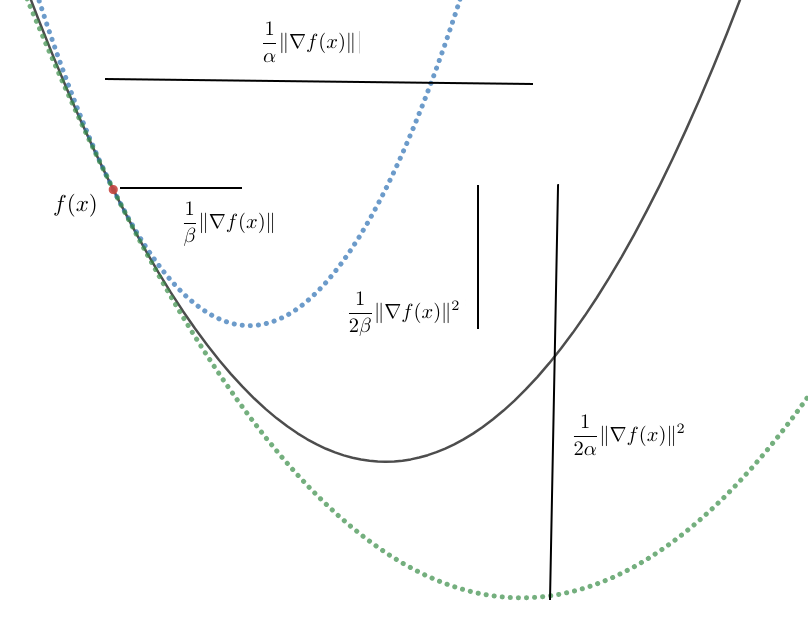
\includegraphics[width=0.5\textwidth]{img/parabolas} 
        \caption{Visualization of the smoothness bound (blue) and the strong convexity bound (green) of a function $f$ (black). }
\end{figure}

We make two important remarks about the previous analysis. Firstly, gradient descent uses the assumption of $\beta$-smoothness to guarantee maximal local decrease and secondly, the guaranteed decrease is better if the norm of the gradient is large. We will note later that the regret of mirror descent is lower when the norm of the gradient is low, and this, along with the second remark, is what we can leverage to combine gradient and mirror descent. But let's focus first on the first remark. The maximal decrease on the objective we can guarantee from $x_k$ occurs when we minimize, as we did before in our toy example, the bound that is given by the $\beta$-smoothness assumption, which is
\[
    f(y) \leq f(x_k) + \langle \nabla f(x_k), y-x_k \rangle + \frac{\beta}{2} \|{y-x_k}\|^2,
\]
for every $y \in \X$. Note that for enough regular functions, the smoothness condition can be derived by upper bounding a second order multivariate Taylor expansion using that the Hessian's eigenvalues are upper bounded by $\beta$. It is a simple way to remember the inequality. So we can define the next point as
 \begin{align}\label{general_grad_descent}
     \begin{aligned}
     x_{k+1} := &\argmin_{y \in \X} \left\{ f(x_k) + \langle \nabla f(x_k), y-x_k \rangle  +\frac{\beta}{2}\|{y-x_k}\|^2\right\} \\
    = &\argmin_{y \in \X} \left\{ \langle \nabla f(x_k), y-x_k \rangle  +\frac{\beta}{2}\|{y-x_k}\|^2\right\}.
    \end{aligned}
\end{align}
If we take $\|{\cdot}\|_2$ and $\X = \R^n$ we are searching for the minimizer in a quadratic function $a y^t y + b^t y + c $, ($a \in \R; b, c \in \R^n$) which is $-\frac{b}{2a}$ or in our case
\[
    -\frac{\nabla f(x_k) - 2 x_k \beta/2}{2 \beta/2} = x_k - \frac{1}{\beta}\nabla f(x_k).
\]
which matches our previous analysis. Maybe the following, for a general convex set $\X$, is more interesting (we subtract constant terms inside the $\argmin$'s):
\begin{align*}
    \argmin_{y \in \X} \left\{ \left\|{\left(x_k - \frac{1}{\beta}\nabla f(x_k)\right) - y}\right\|^2 \right\} \stackrel{?}{=} \argmin_{y \in \X} \left\{ \langle \nabla f(x_k), y-x_k \rangle  +\frac{\beta}{2}\|{y-x_k\|}^2\right\} \\
    \Leftrightarrow \argmin_{y \in \X} \left\{ \langle y, y\rangle - 2\left\langle y, \left(x_k - \frac{1}{\beta} \nabla f(x_k)\right)\right\rangle\right\} \stackrel{?}{=} \argmin_{y \in \X} \left\{ \langle \nabla f(x_k), y\rangle + \frac{\beta}{2}(\langle y, y\rangle - 2\langle x_k, y\rangle)\right\}. \\
\end{align*}
It is clear that the two $\argmin$'s of the last expression are the same, since we can obtain the left hand side by dividing by $\frac{\beta}{2}$ in the $\argmin$ of the right hand side. This means that our rule for projected gradient descent (left hand side) computes the point in $\X$ whose decrease guarantee given by the $\beta$-smoothness of $f$ is maximal among all the points in $\X$ (right hand side). It is natural now to define gradient descent for general norms by rule (\ref{general_grad_descent}). We denote 

\[
    \Prog(x) := - \min_{y\in\X} \left\{ \langle \nabla f(x), y-x \rangle + \frac{\beta}{2} \|{y-x}\|^2\right\} \geq 0.
\]

By the definition of $x_{k+1}$ it is clear that $f(x_{k+1}) \leq f(x_k) - \Prog(x)$ (and $\Prog(x) = \frac{1}{2\beta} \|\nabla f(x)\|_\ast^2$ if $\X = \R^n$). We will call $\Grad(x)$ to the $\argmin$ of the previous expression.

In short, we can say that \textbf{gradient descent at each iteration maximizes the guaranteed local decrease}. 


Our second remark was that with $\X = \R^n$ and $\|\cdot \|_2$ the decrease is better if $\|\nabla f(x)\|$ is larger. An intuition that we will formalize later is that mirror descent for $\X = \R^n$ and $\|\cdot \|_2$ suffers from a small loss if $\|\nabla f(x)\|$ is small. In general we will prove that a bound for the mirror descent loss is going to have a term that will be easy to control and something proportional to $\Prog(x)$. So when mirror descent suffers from a large loss, gradient descent decreases the objective a lot, and when gradient descent does not have a large guaranteed decrease, mirror descent's loss will be small. This is the key idea of linear coupling.

We saw last week that mirror descent tackles the dual optimization problem by constructing lower bounds to the optimum. Recall that each queried gradient $\nabla f(x)$ can be viewed as a hyperplane lower bounding the objective $f$, that is, $f (y) \geq f (x)+ \langle \nabla f (x), y-x \rangle$ for all $y$. Mirror-descent methods attempt to carefully construct a convex combination of these hyperplanes in order to yield even a stronger lower bound. From this point of view our claimed intuition about mirror descent having a small loss when $\|\nabla f(x)\|_2$ is small should be clear, because the planes are closer to being horizontal. We will denote
\[
    \Mirr_{x_k}(\xi):= \argmin_{x \in \X} \left\{ D(x, x_k) + \langle \xi, x-x_k \rangle \right\}. 
\]
Note that a mirror descent step is $x' = \Mirr_{x_k}(\eta \partial f(x_k))$. Here, $D$ is the Bregman divergence of a mirror map $\Phi$ which for simplicity we will assume that is $1$-strongly convex.  \footnote{Note that this is equivalent to the mirror descent step in Algorithm \ref{alg:mirror_descent}. We defined $x_{k+1}$ to be in $ \Pi_\mathcal{X}^\Phi(y_{k+1}) = \argmin_{x\in\X}D(x, y_{k+1}) = \argmin_{x\in\X}\left\{ \Phi(x) - \Phi(y_{k+1}) - \langle \nabla \Phi(y_{k+1}), x\rangle \right\} = \argmin_{x\in\X}\left\{ \Phi(x) - \langle \nabla \Phi(x_k) - \eta \nabla f(x_k), x\rangle \right\}$ where in the last step we have removed constant terms from the $\argmin$ and used the definition of $\nabla \Phi(y_{k+1})$. On the other hand $\argmin_{x\in\X}\{D_(x, x_k) + \langle \eta \nabla f(x_k), x-x_k \rangle\} = \argmin_{x\in\X}\{\Phi(x)  - \Phi(x_k) - \langle \nabla \Phi(x_k), x-x_k\rangle + \langle \eta \nabla f(x_k), x- x_k \}  = \argmin_{x\in\X}\left\{ \Phi(x) - \langle \nabla \Phi(x_k) - \eta \nabla f(x_k), x\rangle \right\}$ where in the last step we have also removed constant terms. We observe that thus the two expressions lead to the same result. However, the second one (or the simplified version of both for that matter) does not need to obtain $y_{k+1}$ from $\nabla \Phi(y_{k+1})$.}

\begin{figure}[h!] \label{mirror_descent_dual_loss}
\centering
        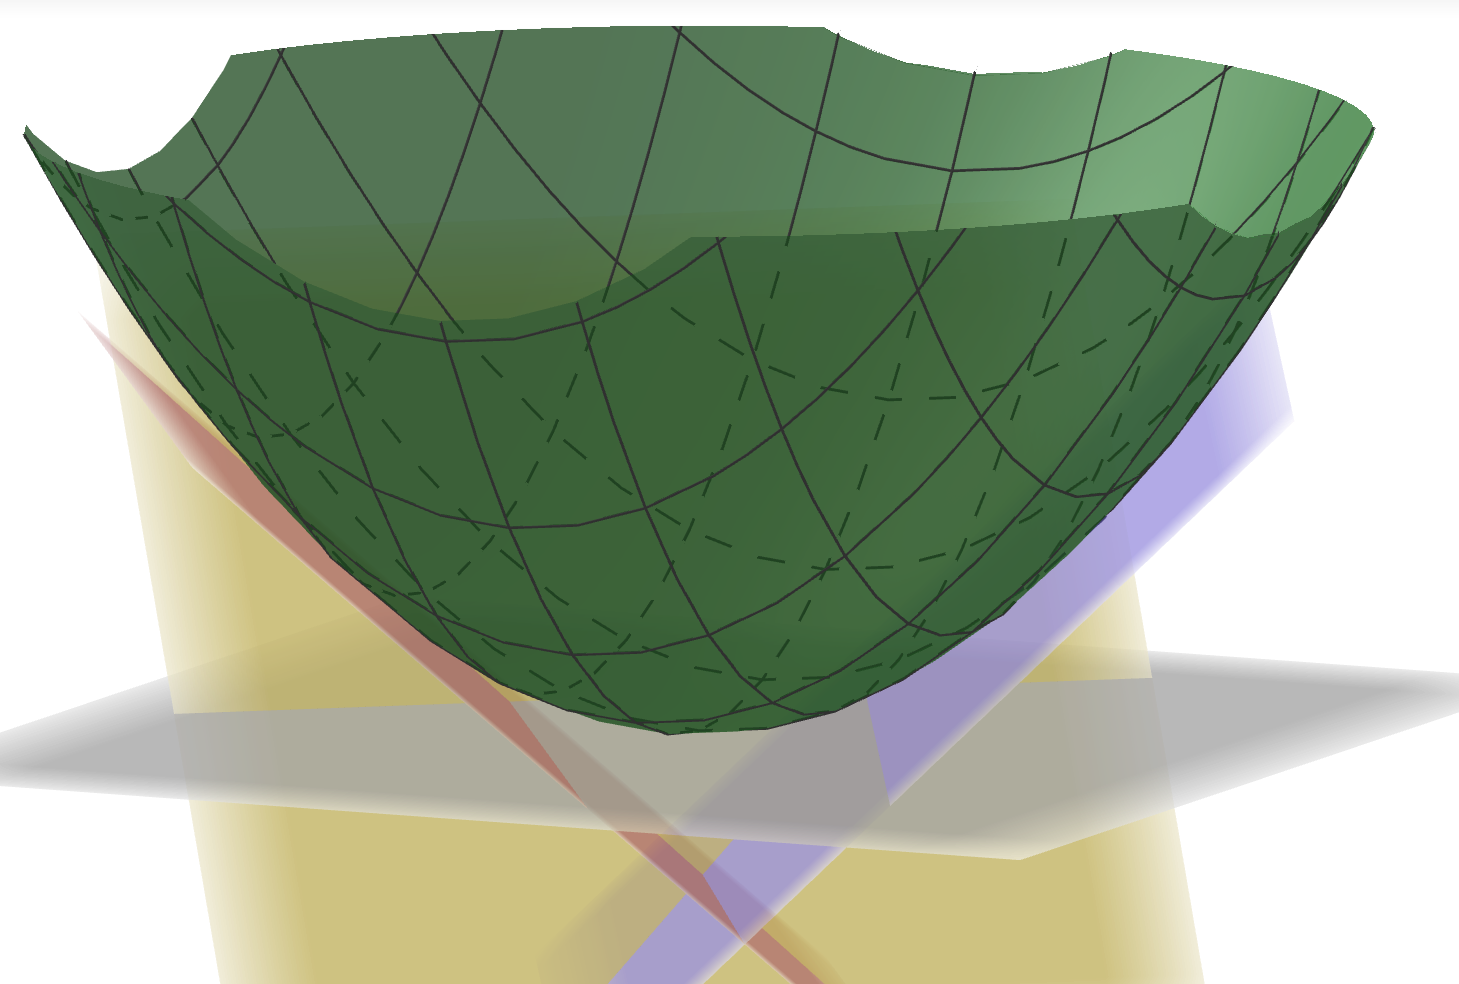
\includegraphics[width=0.5\textwidth]{img/mirror_descent_dual_loss} 
        \caption{Mirror combines several linear lower bounds obtained by convexity to give a lower bound on the optimum.}
\end{figure}

\textbf{Thought experiment.} For the sake of demonstrating the idea, suppose $\| \nabla f(x) \|_2$, the norm of the observed gradient, is \textbf{either} always $\geq K$, or always $\leq K$, where $K$ will be determined later. Under such ``wishful assumption'', we can propose the following algorithm: if the norm of the gradient is always $\geq K$ perform $T$ gradient descent steps. Otherwise perform $T$ mirror descent steps. To analyze such an algorithm, suppose without loss of generality we start with some point $x_0$ whose objective distance $f(x_0 )-f(x^\ast )$ is at most $2\epsilon$, and we want to find some $x$ so that $f(x) - f(x^\ast) \leq \epsilon$.

If $T$ gradient descent steps are performed, the objective decreases by at least $\frac{\|\nabla f(\cdot)\|_2^2}{2\beta} \geq \frac{K^2}{2\beta}$ per step and we only need $T \geq \Omega\left(\frac{\epsilon \beta}{K^2}\right)$ steps to achieve an $\epsilon$ accuracy. If $T$ mirror descent steps are performed, we need $T \geq \Omega\left(\frac{K^2}{\epsilon^2}\right)$ steps according to the mirror descent convergence (Remark \ref{mirror_descent_lemma_for_linear_coupling}). In sum, we need $T \geq \Omega\left( \max \left\{ \frac{\epsilon \beta}{K^2}, \frac{K^2}{\epsilon^2}\right\}\right)$ steps to converge to an $\epsilon$-minimizer. Setting K to be the magic number to balance the two terms, we only need $T \geq \Omega\left( \sqrt{\frac{\beta}{\epsilon}}\right)$ iterations. This means that in the general case in which $f(x_0) - f(x^\ast) \leq d $ we can repeat this procedure to obtain points such that the distances of their images to $f(x^\ast)$ halve after each iteration. So we only need $T \geq \Omega \left(\sqrt{\frac{\beta}{\epsilon}}\left(\sqrt{\frac{2\epsilon}{d}} + \sqrt{\frac{4\epsilon}{d}} + \dots + \sqrt{\frac{1}{2} }+ 1 \right)\right) = \Omega \left( \sqrt{\frac{\beta}{\epsilon}}\right)$.

\section{Warm-Up Method with Fixed Step Length}
The key ideas of this method will be the same as the ones for the final method. As we mentioned previously, at each iteration linear coupling performs a gradient descent step and a mirror descent step and the point for the next iteration is a convex combination of the points obtained by gradient and mirror descent. The key of the proof is to see that the loss in which mirror descent incurs is something proportional to the gradient descent guaranteed decrease (plus a couple of Bregman divergences that will telescope) and using this fact to see that a particular convex combination of mirror and gradient descent incurs in a similar loss.

Formally, we start with $x_0 = y_0 = z_0$. In each iteration $k= 0, 1, \dots, T-1$ we define $x_{k+1} \gets \tau z_k + (1-\tau) y_k$ and then we perform:
\begin{itemize}
    \item A gradient step $y_{k+1} \gets \Grad(x_{k+1})$.
    \item A mirror step $z_{k+1} \gets \Mirr_{z_k}\left(\eta \nabla f(x_{k+1})\right)$.
\end{itemize}
The choices of $\eta$ and $\tau$ will become clear at the end of this section, but from a high level $\eta$ is determined by the mirror descent analysis, similarly to what we saw last week, and $\tau$ will be determined as the best parameter to balance gradient and mirror descent, similar to $K$ in the previous thought experiment.

The two key ideas mentioned before materialize in the following two lemmas:
\begin{lemma}\label{lemma:mirror_bound}
    For every $u \in \X = \R^n$,
    \begin{align}\label{mirror_bound_in_linear_coupling}
        \begin{aligned}
            \eta \langle \nabla f(x_{k+1}), z_k -u \rangle & \leq \frac{\eta^2}{2} \| \nabla f(x_{k+1})\|^2_\ast + D(u, {z_k}) - D(u, {z_{k+1}}) \\
                                                           & \leq \eta^2 \beta (f(x_{k+1}) - f(y_{k+1})) + D(u, {z_k}) - D(u, {z_{k+1}}). \\
        \end{aligned}
    \end{align}
\end{lemma}

\begin{proof}
    The first inequality is Remark \ref{mirror_descent_lemma_for_linear_coupling}, which is the key lemma of the mirror descent analysis. The second inequality is from the gradient step guarantee $f(x_{k+1}) - f(y_{k+1}) \geq \frac{1}{2\beta}\| \nabla f(x_{k+1})\|^2_\ast$.
\end{proof}

The second lemma bounds the actual regret at $x_{k+1}$ and picks $\tau$ so that we can telescope the sum of the regrets.

\begin{lemma}[Coupling]\label{lemma_simplified_coupling} Letting $\tau \in (0, 1)$ satisfy that $\frac{1-\tau}{\tau}  \eta\beta$, we have that
\[
    \forall u \in \X = \R^n, \quad \eta \langle \nabla f(x_{k+1}), x_{k+1} - u \rangle \leq \eta^2\beta\left( f(y_k) - f(y_{k+1})\right) + \left( D(u, {z_k}) - D(u, {z_{k+1}})\right).
\]
\end{lemma}

\begin{proof}
    We can compute easily the difference between the regrets at $x_{k+1}$ and at $z_k$ using the definition of $x_{k+1}$.
    \begin{align}\label{actual_regret_simplified_linear_coupling}
        \begin{aligned}
            \eta \langle \nabla f(x_{k+1}), x_{k+1} - u \rangle - \eta \langle \nabla f(x_{k+1}), z_k - u \rangle = \eta \langle \nabla f(x_{k+1}), x_{k+1} - z_k \rangle  \\
            = \frac{(1-\tau)\eta}{\tau} \langle \nabla f(x_{k+1}), y_k - x_{k+1} \rangle \leq \frac{(1-\tau)\eta}{\tau} (f(y_k) - f(x_{k+1})).
        \end{aligned}
    \end{align}
    Above, we used the fact that $\tau(x_{k+1} - z_k) = (1-\tau)(y_k -x_{k+1})$, as well as the convexity of $f$. It is immediate that by choosing $\frac{1-\tau}{\tau} = \eta \beta$ and combining \eqref{mirror_bound_in_linear_coupling} and \eqref{actual_regret_simplified_linear_coupling} we have the result.
\end{proof}

If we telescope \ref{lemma_simplified_coupling} for $k= 0, 1, \dots, T-1$ and setting $\bar{x} := \frac{1}{T} \sum_{k=0}^{T-1} x_k$  and $u = x^\ast$, we have
\begin{equation}\label{final_lemma_simplified_coupling}
    \eta T \left( f(\bar{x}) - f(x^\ast) \right)\leq \sum_{k=0}^{T-1} \eta \langle \nabla f(x_k), x_k - x^\ast \rangle \leq \eta^2 \beta \left( f(y_0) - f(y_T) \right) + D(x^\ast, x_0) - D(x^\ast, {x_T}).
\end{equation}

Suppose our initial point is of error at most $d$, that is $f (y_0 ) - f (x^\ast ) \leq d$, and suppose $D(x^\ast, {x_0}) \leq \Theta$, then \eqref{final_lemma_simplified_coupling} gives $f (\bar{x})-f (x^\ast ) \leq \frac{1}{T}\left( \eta \beta d + \Theta/\eta\right)$. Choosing $\eta = \sqrt{\Theta/(\beta d)}$ to be the value that balances the above two terms (it is essentially the same way of choosing $\eta$ in mirror descent), we obtain that $f (x) - f (x^\ast ) \leq \frac{\sqrt{\beta \Theta d}}{T}$. In other words, in $T = 4 \sqrt{\beta\Theta/d}$ steps, we can obtain some $\bar{x}$ satisfying $f (\bar{x}) - f (x^\ast ) \leq d/2$, halving the distance to the optimum. If we restart this entire entire procedure a few number of times, halving the distance for every run, then we obtain an $\epsilon$-approximate solution in
\[
    T = O \left(\sqrt{\beta \Theta / \epsilon} + \sqrt{\beta \Theta / 2\epsilon} + \sqrt{\beta \Theta / 4 \epsilon} + \dots \right) = O\left(\sqrt{\beta\Theta / \epsilon}  \right)
\]
iterations. The value of $\eta = \sqrt{\Theta/(\beta d)}$ increases as time goes and therefore $\tau = \frac{1}{\eta \beta +1}$ decreases as time goes. This tells us that gradient descent is given more weight the mirror step when we are close to the minimum.  This fact can be counter-intuitive because when it is closer to the optimum, the observed gradients will become smaller, and therefore mirror steps should perform well according to the thought experiment. This understanding is incorrect, the reason is that when it is closer to the optimum, the threshold between large and small gradients also becomes smaller, so one cannot rely only on mirror steps.

\section{Final Method with Variable Step Lengths}
This final method will change $\eta$ and $\tau$ gradually to obtain an algorithm that does not need to know the bounds $\Theta$ and $d$. This approach will also work for any convex restriction set $\X$. The final algorithm is the following:

\begin{algorithm}[H]\label{alg:AGM}
\scriptsize
\caption{AGM $(f, \Phi, x_0, T)$}
   \label{alg:AGM}
   \begin{algorithmic}[1]
   \REQUIRE $f$ a differentiable and convex function on $\X$ that is $\beta$-smooth with respect to $\|\cdot\|$, $\Phi$ the $DGF$ function that is $1$-strongly convex with respect to the same $\|\cdot\|$ over $\X$. $x_0$ some initial point and $T$ the number of iterations.
   \ENSURE $y_T$ such that $f(y_T) -f(x^\ast) \leq \frac{4\Theta \beta}{T^2}$.
   \STATE $D(y, x) := \Phi(y) - \langle \nabla \Phi(x), y-x\rangle - \Phi(x).$
   \STATE $y_0 \gets x_0, \quad z_0 \gets x_0$.
   \FOR{$ k \gets 0 $ to $T-1$}
       \STATE $\eta_{k+1} \gets \frac{k+2}{2\beta}$, and $\tau_k \gets \frac{1}{\eta_{k+1}\beta} = \frac{2}{k+2}$
       \STATE $x_{k+1} \gets \tau_k z_k + (1-\tau_k)y_k$.
       \STATE {$y_{k+1} \gets \Grad(x_{k+1})$ \hfill\hfill $\left( := \argmin_{y\in\X} \left\{ \frac{\beta}{2} \| y-x_{k+1}\|^2 + \langle \nabla f(x_{k+1}), y-x_{k+1} \rangle \right\}\right) $}
       \STATE{ $z_{k+1} \gets \Mirr_{z_k}\left(\eta_{k+1} \nabla f (x_{k+1})\right)$ \hfill\hfill $\left( := \argmin_{z\in\X} \left\{ D(z, {z_k}) + \langle \eta_{k+1} \nabla f(x_{k+1}), z-z_k \rangle \right\}\right) $}

   \ENDFOR
   \STATE {\bfseries return} $y_T$
\end{algorithmic}
\end{algorithm}

We will prove that this method is accelerated. In particular, we have the following theorem.

\begin{theorem}\label{thm:linear_coupling}
    If $f(x)$ is $\beta$-smooth w.r.t. $\|\cdot\|$ on $\X$, and $\Phi(x)$ is $1$-strongly convex w.r.t. $\|\cdot\|$ on $\X$, then Algorithm \ref{alg:AGM} outputs $y_T$ satisfying $f(y_T) - f(x^\ast) \leq 4 \Theta \beta /T^2$, where $\Theta$ is any upper bound on $D(x^\ast, x_0)$.
\end{theorem}

We will use two lemmas, that are the analogous to Lemma \ref{lemma:mirror_bound} and Lemma \ref{lemma_simplified_coupling}, that we will prove after the proof of the theorem.

\begin{lemma}\label{lemma:mirror_bound_general}
    If $\tau_k = \frac{1}{\eta_{k+1}\beta}$, then linear coupling satisfies that for every $u \in \X$,
    \begin{align*}
        \begin{aligned}
            \eta_{k+1} \langle \nabla f(x_{k+1}), z_{k} - u \rangle &\leq \eta^2_{k+1}\beta \Prog(x_{k+1}) + \left( D(u, z_k) - D(u, z_{k+1})\right) \\
                                                                &\leq \eta_{k+1}^2\beta \left( f(x_{k+1}) - f(y_{k+1})\right) + \left( D(u, z_k) - D(u, z_{k+1})\right).
        \end{aligned}
    \end{align*}
\end{lemma}

\begin{lemma}[Coupling]\label{lemma:coupling} For any $u\in\X$,
    \[
        \left(\eta_{k+1}^2 \beta \right) f(y_{k+1}) - \left( \eta^2_{k+1} \beta - \eta_{k+1}\right)f(y_k) + \left( D(u, z_{k+1} ) - D(u, {z_k})\right) \leq \eta_{k+1} f(u).
    \]
\end{lemma}

\begin{proof}[Proof of Theorem \ref{thm:linear_coupling}]
    In order to telescope Lemma \ref{lemma:coupling} we only need to set the sequence of $\eta_k$ so that $\eta_k^2 \beta \approx \eta_{k+1}^2 \beta - \eta_{k+1}$ as well as $\tau_k = 1/\eta_{k+1}\beta \in (0, 1]$. In Algorithm \ref{alg:AGM} $\eta_k =  \frac{k+1}{2\beta}$ so that $\eta_k^2\beta = \eta^2_{k+1}\beta -\eta_{k+1} + \frac{1}{4\beta}$. Summing up Lemma \ref{lemma:coupling} for $k = 0, 1, \dots, T-1$, we obtain
\[
    \eta^2_T \beta f(y_T) + \sum_{k=1}^{T-1}\frac{1}{4\beta}f(y_k) + \left( D(u, {z_T}) - D(u, {z_0})\right) \leq   \sum_{k=1}^T \eta_k f(u).
\]
By choosing $u= x^\ast$, we notice that $\sum_{k=1}^T \eta_k = \frac{T(T+3)}{4\beta}$, $f(y_k) \geq f(x^\ast)$, $D(u, {z_T}) \geq 0$ and $D(x^\ast, {z_0}) \leq \Theta$. Therefore, we obtain
\[
    \frac{(T+1)^2}{4\beta^2}\beta f(y_T) \leq \left(  \frac{T(T+3)}{4\beta} - \frac{T-1}{4\beta}\right)f(x^\ast) + \Theta,
\]
which after simplification implies $f(y_T)\leq f(x^\ast) + \frac{4\Theta \beta}{(T+1)^2}$.
\end{proof}


\begin{proof}[Proof of Lemma \ref{lemma:mirror_bound_general}]
    The second inequality of the lemma is again by the gradient descent guarantee $f(x_{k+1}) - f(y_{k+1})) \geq \Prog(x_{k+1})$. To prove the first one, we first write down the key inequality of mirror-descent analysis (whose proof is identical to the one given in the previous section). 
\begin{align*}
    \begin{aligned}
        \eta_{k+1} \langle \nabla f(x_{k+1}), z_{k} - u \rangle &= \langle \eta_{k+1} \nabla f(x_{k+1}), z_k - z_{k+1} \rangle + \langle \eta_{k+1} \nabla f(x_{k+1}), z_{k+1} - u \rangle \\
                                                                &\leq  \langle \eta_{k+1} \nabla f(x_{k+1}), z_k - z_{k+1} \rangle + \langle -\nabla D(u, {z_k}), z_{k+1} - u \rangle \\
                                                                &=  \langle \eta_{k+1} \nabla f(x_{k+1}), z_k - z_{k+1} \rangle + D(u, {z_k}) - D(u, z_{k+1}) + D((z_{k+1}, {z_k}) \\
                                                                &\leq  \left( \langle \eta_{k+1} \nabla f(x_{k+1}), z_k - z_{k+1} \rangle - \frac{1}{2}\|z_k - z_{k+1}\|^2 \right)  +  \left( D(u, {z_k}) - D(u, z_{k+1}) \right) \\
    \end{aligned}
\end{align*}
The first inequality is due to the minimality of $z_{k+1} = \argmin_{z\in\X} \{D(u, {z_k}) + \langle \eta_{k+1} \nabla f(x_{k+1}), z \rangle\}$, which implies that  $\langle \nabla D(z_{k+1}, {z_k} ) + \eta_{k+1} \nabla f(x_{k+1}), u-z_{k+1} \rangle \geq 0 $ for all $u \in \X$. The second inequality is because $D(y, x) \geq \frac{1}{2} \|x-y\|^2$ by the strong convexity of the $\Phi(\cdot)$. If we apply Cauchy-Schwarz to the first summand of the last expression above and the fact that $az-bz^2 \leq \frac{a^2}{4b}, \ \forall z \in \R$ we get
\[
    \left( \langle \eta_{k+1} \nabla f(x_{k+1}), z_k - z_{k+1} \rangle - \frac{1}{2}\|z_k - z_{k+1}\|^2 \right) \leq \left(\eta_{k+1}\|\nabla f(x_{k+1})\|_\ast \right) \|z_k - z_{k+1}\| - \frac{1}{2}\|z_k - z_{k+1}\|^2 \leq \frac{\eta_{k+1}^2}{2} \|\nabla f(x_{k+1})\|_\ast^2
\]
and thus we have the result for $\X = \R^n$. For the general constrained we need to use the special choice of $\tau_k = 1/\eta_{k+1} \beta$ as follows. Letting $v:= \tau_k z_{k+1} + (1-\tau_k) y_k \in \X$ so that $x_{k+1} - v = (\tau_k z_k + (1-\tau_k)y_k) -v = \tau_k(z_k-z_{k+1})$, we have
\begin{align*}
     \begin{aligned}
        &\langle \eta_{k+1} \nabla f(x_{k+1}), z_k - z_{k+1} \rangle - \frac{1}{2}\|z_k - z_{k+1}\|^2  \\
        = & \left\langle \frac{\eta_{k+1}}{\tau_k} \nabla f(x_{k+1}), x_{k+1} - v \right\rangle - \frac{1}{2\tau_k^2} \|x_{k+1} - v \|^2 \\
        = & \eta_{k+1}^2 \beta \left( \langle \nabla f(x_{k+1}), x_{k+1} -v \rangle - \frac{\beta}{2} \|x_{k+1} - v\|^2\right) \leq \eta_{k+1}^2 \beta \Prog(x_{k+1})
    \end{aligned}
\end{align*}
where the last inequality is from the definition of $\Prog(x_{k+1})$.

\end{proof}


\begin{proof}[Proof of Lemma \ref{lemma:coupling}]
We can derive the lemma from the following inequalities
\begin{align}
    \begin{aligned}
        &\ \eta_{k+1}(f(x_{k+1}) -f(u)) \\
        \leq &\ \eta_{k+1} \langle \nabla f(x_{k+1}), x_{k+1} -u \rangle \\
        = &\ \eta_{k+1} \langle \nabla f(x_{k+1}), x_{k+1} -z_{k} \rangle + \eta_{k+1} \langle \nabla f(x_{k+1}), z_k -u \rangle \\
        = &\ \frac{(1-\tau_k)\eta_{k+1}}{\tau_k} \langle \nabla f(x_{k+1}), y_k - x_{k+1} \rangle + \eta_{k+1} \langle \nabla f(x_{k+1}), z_k - u \rangle \\
        \leq &\ \frac{(1-\tau_k)\eta_{k+1}}{\tau_k}(f(y_k)-f(x_{k+1})) + \eta_{k+1} \langle \nabla f(x_{k+1}), z_k-u \rangle \\
        \leq &\ \frac{(1-\tau_k)\eta_{k+1}}{\tau_k}(f(y_k)-f(x_{k+1})) + \eta_{k+1}^2 \beta (f(x_{k+1}) - f(y_{k+1}))  + D(u, {z_k}) - D(u, z_{k+1})\\
            = &\ (\eta_{k+1}^2\beta -\eta_{k+1})f(y_k) -(\eta_{k+1}^2 \beta)f(y_{k+1})  +\eta_{k+1}f(x_{k+1})   + \left( D(u, {z_k}) - D(u, z_{k+1})\right)\\
    \end{aligned}
\end{align}
where the lines $4,5,6$ and $7$ are obtained, respectively, by $(4)$ the choice of $x_{k+1}$ that satisfies $\tau_k(x_{k+1} - z_k) = (1-\tau_k) (y_k - x_{k+1})$; $(5)$ is by the convexity of $f$ and $1-\tau_k \geq 0$; $(6)$ uses Lemma \ref{lemma:mirror_bound_general} and $(7)$ uses the choice of $\tau_k = 1/\eta_{k+1}\beta$.
\end{proof}

\textbf{Conclusion.} Linear coupling describes a family of methods whose oracle complexity matches the lower bound that we had proved for these kinds of algorithms. However, this is not the end of the story. Linear coupling provides intuition about acceleration as any other method before. The authors of the paper advocate thinking about any kind of first order optimization problem in terms of linear coupling. Provided one proves similar lemmas for the guaranteed progress of the primal approach (gradient descent) and for the loss of the dual approach (mirror descent) for your particular problem, one can try to use linear coupling to obtain a fast algorithm. Since Linear Coupling was published, there have been several proposals of algorithms to solve optimization problems whose complexity is lower than the one of the best previous known algorithm. Some of these are: the first accelerated stochastic gradient descent algorithm \cite{allen2016katyusha}, a faster algorithm for matrix scaling \cite{allen2017much}, a faster algorithm of accelerated coordinate descent using non-uniform sampling \cite{allen2016even}, nearly-linear time packing and covering LP solvers \cite{allen2014nearly}, an algorithm to solve positive LPs faster in parallel \cite{allen2014using}, an algorithm for non-convex optimization faster than stochastic gradient descent \cite{allen2017natasha}.

%! TEX root = main.tex

\section{Non-Euclidean setting: Frank-Wolfe}
\emph{Speaker: Chris Carmona, 23/10/2017.}\\

The \emph{Conditional Gradient Descent} method, also known as \emph{Frank-Wolfe} is an iterative first-order optimization algorithm for constrained convex optimization, originally proposed in \cite{Frank1956} by Marguerite Frank and Philip Wolfe, then post-docs working in the Princeton logistics project led by Kuhn and Tucker. In recent years, Frank-Wolfe-type methods have re-gained interest, started by the valuable insights provided by \cite{Jaggi2013}, and fuelled by its good scalability and convergence properties properties (eg. convergence invariance under affine transformations).

The method addresses general constrained convex optimization problems of the form $\min_{x \in \X} f(x)$. It assumes that the objective function $f$ is convex and continuously differentiable, and that the domain $\X$ is a compact convex subset of any vector space. Procedure \ref{alg:frank_wolfe} describes the method. In each iteration, the algorithm considers a linear approximation of the objective function, and moves towards a minimizer of this linear function, taken over the domain $\X$. Figure \ref{fig:frank_wolfe} illustrates one iteration of the algorithm (the domain $\X$ is denoted by $\mathcal{D}$ here).

\begin{algorithm}
%\scriptsize
\caption{Conditional Gradient Descent (Frank-Wolfe)}
   \begin{algorithmic}[1] \label{alg:frank_wolfe}
   \REQUIRE $f$ a differentiable and convex function on $\X$ that is $\beta$-smooth w.r.t. some norm $\|\cdot\|$.
   \ENSURE $x_T$ such that $f(x_T)-f(x^\ast) \leq \frac{4 \beta R^2 }{T+1}$ with $R = \sup_{x,y \in \X} \| x - y\|$
   
   \STATE Let $x_{0} \in \X$
   \FOR {$t \in 0,\ldots,T$}
      \STATE Set $\gamma_t=\frac{2}{t+2}$
      \STATE Compute
      \begin{equation} \label{eq:fw_update}
      s_t:= \argmin_{s \in \X } \langle s, \nabla f(x_t) \rangle
      \end{equation}
      \STATE Update $x_{t+1} := (1-\gamma)x_t+ \gamma s_t = x_{t} + \gamma(s_t-x_t)$
   \ENDFOR
   \STATE {\bfseries return} $x_T$
\end{algorithmic}
\end{algorithm}

From a computational perspective, a key property of this scheme is that it replaces the projection step of projected gradient descent by a linear optimization over $\X$ , which in some cases can be a
much simpler problem.

\begin{figure}[ht]
\begin{center}
   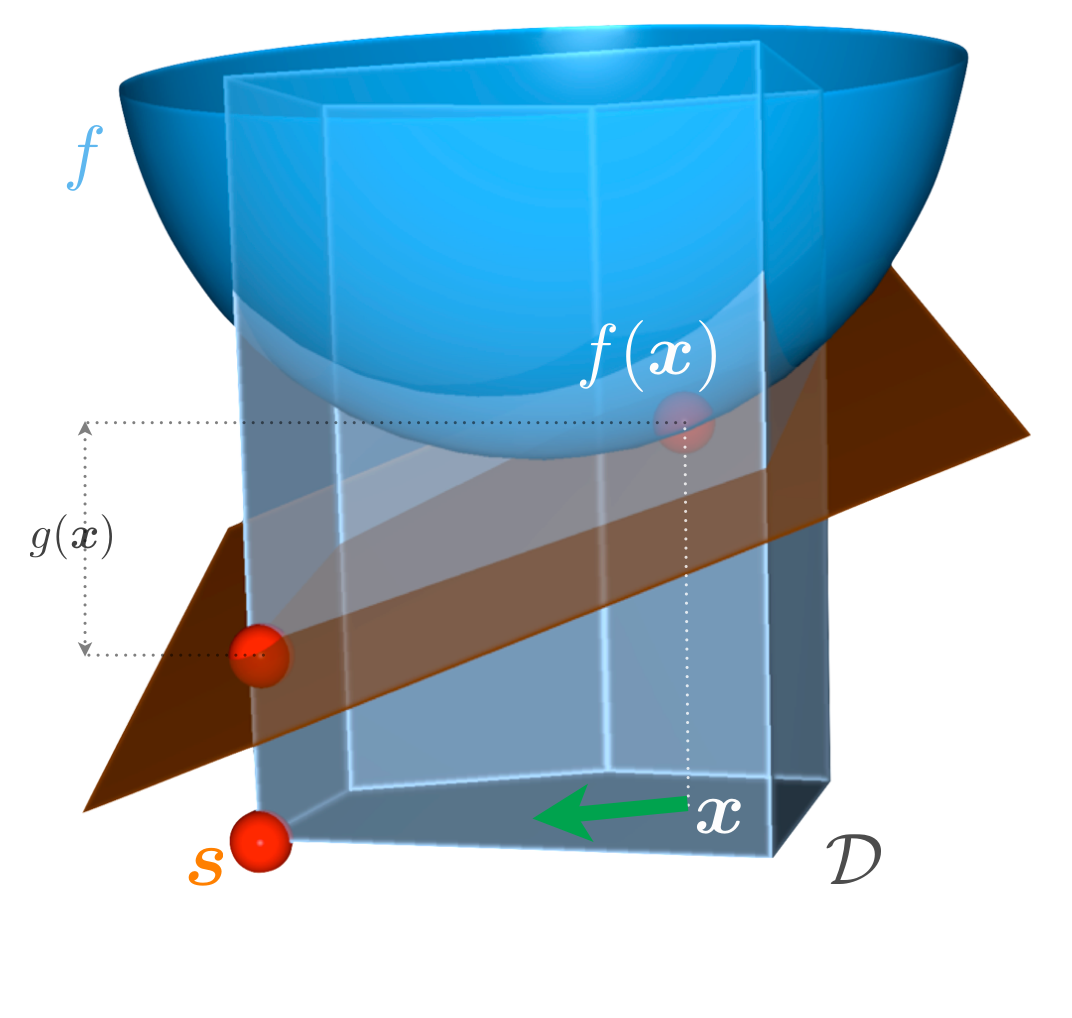
\includegraphics[width=0.5\textwidth]{img/frank_wolfe}
\end{center}
   \caption{Graphical representation of the Conditional Gradient Descent algorithm \cite{Jaggi2013}}
   \label{fig:frank_wolfe}
\end{figure}


\subsection{Convergence analysis.}

A major advantage of conditional gradient descent over projected gradient descent is that the former can adapt to smoothness in an arbitrary norm.

\if
The convergence analysis of Frank-Wolfe type algorithms crucially relies on a measure of “non-linearity” of our objective function f over the domain $\X$. The \emph{curvature constant} $C_f$ of a convex and differentiable function $f:\mathbb{R}^n \rightarrow \mathbb{R}$, with respect to a compact domain $\X$ is defined as:

\begin{equation} \label{eq:curv_const}
C_f := \sup_{ \substack{x,s \in \X,\\ \gamma \in [0,1],\\ y=x+\gamma(s-x)} } \frac{2}{\gamma^2} (f(y)-f(x)-\nabla f(x)^\top (y-x))
\end{equation}

Note that $C_f$ actually measures how far $f$ is from being linear, getting $C_f=0$ when $f$ is linear. The quantity $f(y)-f(x)-\nabla f(x)^\top (y-x)$ is called the \emph{Bregman divergence} defined by $f$.
\fi

The following theorem establishes a bound of convergence. Note that the number of iterations needed to have $f(x_t)-f(x^*) \leq \epsilon$  is $O(\frac{1}{\epsilon})$.

\begin{theorem}
Let f be a convex and $\beta$-smooth function w.r.t. some norm $\|\cdot\|$, $R=\sup_{x,y \in \X} \| x-y \|$, and $\gamma_t=\frac{2}{t+1}$ for $t \geq 1$. Then for any $t\geq2$, one has:
\begin{equation}
f(x_t)-f(x^*) \leq \frac{4 \beta R^2 }{t+1}
\end{equation}
\end{theorem}

\begin{proof}
First, note that the following inequalities hold:
  \begin{align}
    f(x_{t+1})-f(x_t) & \leq \nabla f(x_t)^\top (x_{t+1}-x_{t}) + \frac{\beta}{2} \| x_{t+1}-x_{t} \|^2 \nonumber && \text{($f$ is $\beta$-smooth)} \\
    & \leq \gamma_t \nabla f(x_t)^\top (s_{t}-x_{t}) + \frac{\beta}{2} \gamma_t^2 R^2 \nonumber && \text{($x_{t+1}=x_t+\gamma (s_t-x_t)$)} \\
    & \leq \gamma_t \nabla f(x_t)^\top (x^*-x_t) + \frac{\beta}{2} \gamma_t^2 R^2 \nonumber && \text{(by definition $s_t \leq x^*$)} \\
    & \leq \gamma_t ( f(x^*)-f(x_t)) + \frac{\beta}{2} \gamma_t^2 R^2 \nonumber && \text{(convexity of $f$)}
  \end{align}
If we define $\delta_t = f(x_t)-f(x^*)$ then we get:
\begin{equation}
\delta_{t+1} \leq (1-\gamma_t)\delta_t+\frac{\beta}{2} \gamma_t^2 R^2
\end{equation}
Finally, the result is proved by induction using $\gamma_t =\frac{2}{t+1}$. We initialize at step 2, $t=1$, with the above inequality yielding $\delta_2 \leq \frac{\beta}{2} R^2$.
\end{proof}

\subsection{Sparse iterates property.}
In addition to being projection-free and "norm-free", the conditional gradient descent satisfies a perhaps even more important property: it produces \emph{sparse iterates}.

Consider the situation where $\X \subset \mathbb{R}^n$ is a polytope, that is the convex hull of a finite set of points (these points are called the vertices of $\X$ ). Then Caratheodory's theorem states that any point $x \in \X$ can be written as a convex combination of at most $n+1$ vertices of $\X$ . On the other hand, by definition of the conditional gradient descent, one knows that the $t$-th iterate $x_t$ can be written as a convex combination of $t$ vertices (assuming that $x_1$ is a vertex). Thanks to the dimension-free rate of convergence one is usually interested in the regime where $t<<n$, and thus we see that the iterates of conditional gradient descent are very sparse in their vertex representation.

\subsection{Application: Regularized least-squares regression.}
The three properties of conditional gradient descent (projection-free, norm-free, and sparse iterates) are critical to develop a computationally efficient procedure in solving this kind of problems.

Consider the regularized least-squares regression problem (which includes the LASSO). We would like to approximate a signal $Y \in \mathbb{R}^n$ by using a combination of few of the columns $x_j; j\in 1,\ldots,p$ in the matrix $X \in \mathbb{R}^{n \times p}$. Then, for a fixed $\lambda$ we have the penalized problem in dimension $p$:
\begin{equation}
\min_{\beta \in \mathbb{R}^p} \| Y - X \beta \|_2^2 + \lambda \|\beta\|_1 \nonumber
\end{equation}

Instead of considering the penalized version of the problem one could look at the following constrained problem, with $s \in \mathbb{R}$ fixed:
\begin{align} \label{eq:lasso_fw}
\min_{\beta \in \mathbb{R}^p} \| Y/s - X \beta \|_2^2 \\
\text{subject to} \|\beta\|_1 \leq 1 \nonumber
\end{align}

We are interested in situations where $n<<p$, that is the number of variables $p$ in $X$ can be very large, potentially exponential in the dimension $n$. Nonetheless we want to restrict our attention to algorithms that run in reasonable time with respect to $n$, that is we want polynomial time algorithms in $n$. Of course in general this is impossible, and we need to assume that the dictionary has some structure that can be exploited. Here we make the assumption that one can solve in time $p(n)$ (where $p$ is polynomial) the following problem for any $y\in\mathbb{R}$:
\begin{equation}
\min_{ 1\leq i \leq p } y^{\top} x_i\nonumber
\end{equation}
Finally, for normalization issues, we assume that the $\ell_2$-norm of the $x_i$'s are controlled by some $m > 0$, that is $\| x_j \|_2 \leq m, \forall j \in 1,\ldots,p $

Our problem of interest \ref{eq:lasso_fw} corresponds to minimizing the function $f(\beta) = \frac{1}{2}\| Y - X \beta \|_2^2 $ on the $\ell_1$-ball of $\mathbb{R}^p$ in polynomial time in $n$. At first sight this task may seem completely impossible indeed one is not even allowed to write down entirely a vector $\beta \in \mathbb{R}^b$ (since this would take time linear in $p$ ). The key property that will save us is that this function admits sparse minimizers as we discussed above, and this will be exploited by the conditional gradient descent method.

Let us study the computational complexity of the $t$-th step of
conditional gradient descent. First, observe that:
\begin{equation}
\nabla f (\beta)=X^\top (X\beta-Y) \nonumber
\end{equation}

Now assume that $s_t=X \beta_t - Y \in \mathbb{R}^n$ is already computed, then to compute the update \ref{eq:fw_update} one needs to find  the coordinate $i_t \in 1,\ldots,p$ that maximizes $| [\nabla f(\beta_t)](i) |$ which can be done by maximizing $x_i^\top s_t$ and $-x_i^\top s_t$. Thus \ref{eq:fw_update} takes time $O(p(n))$. Computing $\beta_{t+1}$ from $\beta_t$ and $i_t$ takes time $O(t)$ since $\|x_t \|_0 \leq t$, and computing $s_{t+1}$ from $s_t$ and $i_t$ takes time $O(n)$. Thus the overall time complexity of running t steps is (we assume $p(n) =\Omega(n)$)
\begin{equation} \label{eq:lasso_time_bound}
O(tp(n) + t^2 )
\end{equation}

To derive a rate of convergence it remains to study the smoothness
of $f$ . This can be done as follows:
\begin{align}
\| \nabla f(\beta) - \nabla f(\gamma) \|_{\infty} & = \| X^\top X(\beta-\gamma) \|_{\infty} \nonumber \\
& = \max_{1 \leq j \leq p} | x_j^\top \sum_{k=1}^{p} x_k(\beta(k)-\gamma(k)) | \nonumber \\
& \leq m^2 \| \beta-\gamma \|_1 \nonumber \\
\end{align}
which means that $f$ is $m^2$-smooth with respect to the $\ell_1$-norm.

Thus we get the following rate of convergence:
\begin{equation} \label{eq:lasso_fw_bound}
f(\beta_t)-f(\beta^*) \leq \frac{8 m^2}{t+1}
\end{equation}

Putting together \ref{eq:lasso_time_bound} and \ref{eq:lasso_fw_bound} we proved that one can get an $\epsilon$-optimal solution to \ref{eq:lasso_fw} with a computational effort of $O(m^2 p(n)/\epsilon+m^4/\epsilon^2)$ using the conditional gradient descent.

\subsection{Frank-Wolfe variants.}

\subsubsection{Line search.}

Instead of using the pre-defined step-sizes $\gamma=\frac{2}{k+2}$ a modified algorithm the best point on the line segment between the current iterate x(k) and s.
\begin{equation}
\gamma_t = \argmin_{\gamma \in [0,1]} f( x_{t-1} + \gamma(s_{t-1}-x_{k-1}) ) \nonumber
\end{equation}

\subsubsection{Fully corrective.}

This is a harder-working variant of the Frank-Wolfe method, which after the addition of a new \emph{atom} (or search direction) $s$ re-optimizes the objective $f$ over all previously used atoms. Here in step $t$, the current atom $s_t$ is still allowed to be an approximate linear minimizer.

Comparing to the original Frank-Wolfe method, the idea is that the variant here will hopefully make more progress per iteration, and therefore result in iterates $x$ being combinations of even fewer atoms (i.e. better sparsity). This however comes at a price, namely that the internal problem in each iteration can now become as hard to solve as the original optimization problem, implying that no global run-time guarantees can be given for the algorithm in general.

\subsubsection{Away steps.}
Another important variant is the use of \emph{away-steps}. The idea is that in each iteration, we not only add a new atom $s$, but potentially also remove an old atom (provided it is bad with respect to our objective). This requires that the iterate $x$ is represented as a convex combination of the current atoms. This variant can improve the sparsity of the iterates. Using away-steps, a faster linear convergence can be obtained for some special problem class.

\subsubsection{Inexact updates.}
Jaggi (2011) also analyzes inexact Frank-Wolfe updates.

Suppose we choose $s_t$ with some "small" inaccuracy so that:
\begin{equation}
      \langle s_t, \nabla f(x_t) \rangle = \min_{s \in \X } \langle s, \nabla f(x_t) \rangle + \delta \frac{\gamma_{t+1}C_f}{2}
\end{equation}

where $\delta$ is our \emph{inaccuracy parameter}. $C_f$ is known as the \emph{curvature constant}, measures how far $f$ is from being linear, getting $C_f=0$ when $f$ is linear, and defined as:
\begin{equation} \label{eq:curv_const}
C_f := \sup_{ \substack{x,s \in \X,\\ \gamma \in [0,1],\\ y=x+\gamma(s-x)} } \frac{2}{\gamma^2} (f(y)-f(x)-\nabla f(x)^\top (y-x))
\end{equation}


In \cite{Jaggi2013} it is shown that the attained rate of convergence is basically the same under this \emph{inexact updates}.

\begin{theorem}
The Conditional Gradient Method using fixed step $\gamma_t=\frac{2}{t+2}$ sizes and inaccuracy parameter $\delta \geq 0$,
satisfies
\begin{equation}
f(x_t)-f(x^*) \leq \frac{2 C_f }{t+2} (1+\delta)
\end{equation}
\end{theorem}
%!TEX root = optimization1718.tex

\chapter{Stochastic oracle model}
\emph{Speaker: Adam Foster, 30/11/2017.}\\

Assume that we want to solve the following problem:
\begin{align*}
	\begin{aligned}
		\text{minimize }\quad   & f(x) \\
		\text{subject to }\quad & x\in \mathcal{X},
	\end{aligned}
	\label{def:stochastic problem}
\end{align*}
where $f$ is a convex function, possibly not known. In previous work, we assumed that we had a first order oracle which, given $x \in \mathcal{X}$, would yield a $g \in \partial f(x)$. When analysing our algorithms in terms of oracle complexity, it was the \textit{number of calls} to the oracle that was important. In many applications, an oracle may not exist, or a single call to the oracle may be very expensive. In such cases, we accept randomness in our oracle but require it to be unbiased.

Formally, a first order \emph{stochastic} oracle model defines the framework where given $x\in\mathcal{X}$ an oracle yields back a random variable $G$ that is an unbiased estimator of a subgradient of $f$ at $x$, namely, $\E[G] \in \partial f(x)$. If $X$ is a random variable, the oracle yields back a random variable $G$ that is an unbiased estimator of a subgradient of $f$ at $X$ conditionally on $X$, namely, $\E[G|X] \in \partial f(X)$.


\section{Projected gradient descent with a stochastic oracle}
We analyse the behaviour of the projected gradient descent algorithm to solve problem \eqref{def:stochastic problem} when we replace exact knowledge of subgradients of $f$ with unbiased estimates of them. For a given initial point $X_1\in\X$, possibly random, and a given collection of step sizes $\eta_1,\eta_2,\ldots$, the stochastic projected gradient descent is defined by the sequence of random variables generated according to the following update:
\begin{align*}
Y_{s+1} &= X_s - \eta_s G_s,\\
X_{s+1} &= \Pi_{\X}(Y_{s+1}).
\end{align*}
where $G_s$ is obtained from a stochastic oracle with $\E[G_s|X_s] \in \partial f(X_s)$.

Remarkably, for $f$ a $L$-Lipschitz function we can recover the rate of convergence of the deterministic oracle (cf. Theorem \ref{thm:projectedgradL}). When $f$ is additionally $\alpha$-strongly convex we recover the unaccelerated rate of convergence of \cite{bubeck} Theorem 3.9.

\begin{theorem}[$L$-Lipschitz Stochastic Projected Subgradient Descent]
\label{thm:projectedgradLstoch}
Let $f$ be convex. Suppose $\X$ is contained in a Euclidean ball of radius $B$ centred at $X_1$. Suppose that for every $X \in \X$ the stochastic oracle yields an unbiased estimator of the subgradient of $f$ at $X$ bounded in $L_2$, namely, $\E[G |X]\in \partial f(X)$ and $\E[\|G\|^2] \leq L^2$. Then, the projected subgradient descent method with $\eta_s\equiv\eta = \frac{B}{L\sqrt{t}}$ satisfies 
\begin{equation} \label{eqn:proj_subgrad_t stoch}
\E f\left(\frac{1}{t} \sum_{s=1}^t X_s\right) - f(x^*) \leq \frac{LB}{\sqrt{t}}.
\end{equation}
\begin{proof}
For any $1 \leq s \leq t$ we have
\begin{align*}
	f(X_s) - f(x^*)
	\le \E [G_s|X_s]^T(X_s - x^*)
	= \E [G_s^T(X_s - x^*)|X_s].
\end{align*}

Proceeding as in the proof of Theorem \ref{thm:projectedgradL}, we find
\begin{align*}
	G_s^T(X_s - x^*)
	\le \frac{1}{2\eta} \left( \|X_s - x^*\|^2 - \|X_{s+1} - x^*\|^2 \right) + \frac{\eta}{2} \|G_s\|^2.
\end{align*}

Taking the expectation, we get
\begin{align*}
	\E f(X_s) - f(x^*) &\leq 
	\E [G_s^T(X_s - x^*)]
	\le \frac{1}{2\eta} \left( \E\|X_s - x^*\|^2 - \E\|X_{s+1} - x^*\|^2 \right) + \frac{\eta}{2} \E[\|G_s\|^2],
\end{align*}
and using the assumption $\E[\|G_s\|^2]\le L^2$ we get
\[
\frac{1}{t} \sum_{s=1}^t (\E f(X_s) - f(x^*)) \leq \frac{1}{2 \eta t} \left( \E\| X_1 - x^* \|^2 - \E\| X_{t+1} - x^* \|^2 \right) + \frac{\eta}{2} L^2 \leq \frac{B^2}{2 \eta t} + \frac{\eta L^2 }{2}.
\]

Selecting $\eta = \frac{B}{L\sqrt{t}}$ to minimize the right-hand side of the above inequality gives the first result in \eqref{eqn:proj_subgrad_t} (since $f\left(\frac{1}{t}\sum_{s=1}^t X_s \right) \leq \frac{1}{t} \sum_{s=1}^t f(X_s)$ by Jensen's inequality).
\end{proof}
\end{theorem}



\begin{theorem}[$\alpha$-strongly convex Stochastic Projected Subgradient Descent]
\label{thm:projectedgradalphastoch}
Let $f$ be $\alpha$-strongly convex. Suppose that for every $X \in \X$ the stochastic oracle yields an unbiased estimator of the subgradient of $f$ at $X$ bounded in $L_2$, namely, $\E[G |X]\in \partial f(X)$ and $\E[\|G\|^2] \leq L^2$. Then, the projected subgradient descent method with $\eta_s = \frac{2}{\alpha(s+1)}$ satisfies 
\begin{equation} \label{eqn:proj_subgrad_alpha stoch}
\E f\left( \sum_{s=1}^t \frac{2s}{t(t+1)}X_s \right) - f(x^*) \leq \frac{2L^2}{\alpha(t+1)}.
\end{equation}
\begin{proof}
For any $1 \leq s \leq t$ we have
\begin{align*}
	f(X_s) - f(x^*)
	\le \E [G_s|X_s]^T(X_s - x^*) - \frac{\alpha}{2}\|X_s - x^*\|^2
	= \E \left[G_s^T(X_s - x^*) - \frac{\alpha}{2}\|X_s - x^*\|^2 \large| X_s \right].
\end{align*}

Proceeding as before, we find
\begin{align*}
	G_s^T(X_s - x^*) - \frac{\alpha}{2}\|X_s - x^*\|^2
	\le \left( \frac{1}{2\eta_s} - \frac{\alpha}{2} \right) \|X_s - x^*\|^2 - \frac{1}{2\eta_s}\|X_{s+1} - x^*\|^2 + \frac{\eta_s}{2} \|G_s\|^2.
\end{align*}

Taking the expectation and applying $\E[\|G_s\|^2] \le L^2$ gives
\begin{align*}
	\E f(X_s) - f(x^*)
	\le \left( \frac{1}{2\eta_s} - \frac{\alpha}{2} \right) \E[\|X_s - x^*\|^2] - \frac{1}{2\eta_s}\E [\|X_{s+1} - x^*\|^2] + \frac{\eta_s L^2}{2}.
\end{align*}

Multiplying by $s$ and using $\eta_s = \frac{2}{\alpha(s+1)}$ we get
\begin{align*}
	s(\E f(X_s) - f(x^*))
	\le \frac{\alpha}{4}s(s-1) \E[\|X_s - x^*\|^2] - \frac{\alpha}{4}s(s+1) \E [\|X_{s+1} - x^*\|^2] + \frac{L^2}{\alpha},
\end{align*}
which upon summing over $s$ leads to
\[
\sum_{s=1}^t s(\E f(X_s) - f(x^*)) \le \frac{tL^2}{\alpha} + \text{(telescopes)}.
\]

By multiplying through by $\frac{2}{t(t+1)}$ and applying Jensen's inequality to $f$ we have \eqref{eqn:proj_subgrad_alpha stoch}.
\end{proof}
\end{theorem}

Theorem \ref{thm:projectedgradLstoch} shows that, in expectation, the stochastic projected subgradient descent method yields the same convergence guarantees as the deterministic counterpart analysed in Theorem \ref{thm:projectedgradL}.  In particular, the oracle complexity is the same\footnote{Note that different notions of accuracy are used, however, as we consider the expected value of the stochastic method.}: to get an accuracy $\varepsilon$, both methods requires $O(1/\varepsilon^2)$ calls to their respective oracles. The main advantage of the stochastic version lies in the fact that in some applications the \emph{computational} complexity involved in having access to a stochastic oracle is much cheaper than in the deterministic case. We now show that the stochastic model yields substantial computational saving in machine learning.

\section{Expected risk minimization and empirical risk minimization revisited}
Let us recall the original problem that motivates us in Section \ref{sec:intro}, namely, the expected risk minimization:
\begin{align*}
	\begin{aligned}
		\text{minimize }\quad   & r(x) = \E\ell(x^T\Phi(W),Y) \\
		\text{subject to }\quad & x\in \mathcal{X}.
	\end{aligned}
\end{align*}
The assumption here is that we know the loss function $\ell$ (indeed, we can choose it!) and the constraint set $\mathcal{X}$, but we do not know the distribution of $(W,Y)$. We only have access to $m$ i.i.d.\ samples $(W_1,Y_1),\ldots,(W_m,Y_m)$ from this unknown distribution.

With the concept of a stochastic oracle in hand, one can now attack the expected risk minimization problem directly because $G \in \partial R_i$ is an unbiased estimator of the subgradient of $r$ where $R_i(x) = \ell(x^T\Phi(W_i), Y_i)$. Using this method, one can hope to solve the problem exactly. However, to ensure unbiasedness it is necessary to make only a \textit{single} gradient step with each independent $(W_i, Y_i)$, leading to a single pass through the data. Such an approach is well-suited to an online learning algorithm in which a data is processed and discarded in a stream.

Alternatively, one could minimize the empirical risk $R(x) = \frac{1}{m}\sum R_i(x)$ (see \eqref{def:mainproblem empirical risk}). Proposition~\ref{prop:erm2} shows that the error can be controlled by breaking the resulting error into $STATISTICS$ and $OPTIMIZATION$ terms. Whilst $R$ and its subgradients may be tractable, such computations are typically $O(m)$. Stochastic oracle methods can reduce this to $O(1)$. One could select $I \sim \text{Uniform}(1, ..., m)$ and use $G \in \partial R_I$ as an unbiased estimator of the subgradient of $R$. Since unlimited i.i.d. samples of $I$ are available, multiple passes over the data can be made. The key difference is that the functions being optimized in the two cases are different.

\section{Single pass over the data}
In the expected risk minimization problem we do not know the function $r$ that we want to minimize, and in particular we can not operate in the deterministic first order oracle model discussed in the previous weeks as for a given $x\in\mathcal{X}$ we do not have access to a subgradient in $\partial r(x)$. On the other hand, given $x\in\mathcal{X}$ we can have access to an unbiased estimator of a subgradient of $r$ evaluated at $x$. In fact, given the function $x \mapsto R_i(x) := \ell(x^T\Phi(W_i),Y_i)$, which is known to us, we can compute a subgradient of $R_i$ at $x$. This is a random variable $G_i\in \partial R_i(x)$ that satisfies $\E G_i \in \partial r(x)$. The same is true if we want to get an estimate of the subgradient of $r$ at $X\in\X$ when $X$ is a random variable \emph{independent} of $(W_i,Y_i)$. In fact, in this case we can evaluate a subgradient of $R_i$ at $X$, and this random variable $G_i\in \partial R_i(X)$ satisfies $\E[G_i|X]\in r(X)$.\footnote{Note that if $X$ is random, then there are two sources of randomness in $G_i$: one source is $X$ itself, the other is the data point $(W_i,Y_i)$. The statement $\E[G_i|X]\in \partial r(X)$ holds if $X$ and $(W_i,Y_i)$ are independent.} Hence, we satisfy the assumption of the first order stochastic oracle model. At the same time, as we have $m$ independent data points at out disposal, we can have access to at most $m$ independent unbiased estimators of subgradients evaluated at possibly different locations in $\mathcal{X}$. In other words, the requirement of independence restricts us to a \emph{single pass} over the data, which is not as general as in the stochastic block model defined above where we can have how many queries to the oracle as we want.

It is easy to check that under the assumptions of Proposition \ref{prop:Lip-stats}, Theorem \ref{thm:projectedgradLstoch} yields the following convergence guarantees for the stochastic projected descent method:
$$
	\E r(\hat X_m) - r(x^*) \leq \frac{GL_\textrm{loss}B}{\sqrt{m}},
$$
with $\hat X_m = \frac{1}{m}\sum_{i=1}^m X_i$. The computational savings are clear. If computing a subgradient for each functions $R_i$ costs $O(1)$, then the computational complexity of stochastic gradient descent to achieve precision $\varepsilon$ (in expectation) is of order $O(1/\varepsilon^2)$. On the other hand, if we apply the deterministic gradient descent method to minimize the empirical risk $R$ up to precision $1/\sqrt{m}$, as discussed in Section \ref{sec:intro} and in Remark \ref{rem:optimization}, then we see that the computational complexity is $O(m/\varepsilon^2)$, as we need $O(1/\varepsilon^2)$ calls to the deterministic oracle but each call costs $O(m)$ base iterations, as $R(x) := \frac{1}{m} \sum_{i=1}^m R_i(x)$.

\section{Multiple passes over the data}
In the unconstrained empirical risk minimization problem
\begin{align*}
	\text{minimize }\quad   & R(x) = \frac{1}{m}\sum_{i=1}^m R_i(x)
\end{align*}
we assume henceforth that the $R_i$ are $\beta$-smooth and that $R$ is $\alpha$-strongly convex. Let $\kappa = \beta/\alpha$ which is typically very large. The problem is amenable to basic gradient descent
\begin{equation*}
	x_{t+1}= x_t - \frac{\eta_t}{m}\sum_{i=1}^m \nabla R_i(x),
\end{equation*}
and stochastic gradient descent
\begin{equation*}
	x_{t+1}= x_t - \eta_t \nabla R_{I_t}(x),
\end{equation*}
where $I_t$ are i.i.d $\text{Uniform}(1, ..., m)$. In \cite{bubeck} Theorem 3.10 it is shown that basic gradient descent can achieve an exponential rate $O(m\kappa\log(1/\varepsilon))$ whereas Theorem~\ref{thm:projectedgradalphastoch} showed that stochastic gradient descent achieves $O(1/(\alpha\varepsilon))$.

This motivates Stochastic Variance Reduced Gradient descent (SVRG) algorithm. This is a stochastic oracle method which achieves $O((m+\kappa)\log(1/\varepsilon))$.

The main idea of the algorithm is to introduce a reference $y$ and to compute the deterministic gradient $\nabla R(y)$. In place of $\nabla R_I(x)$ one uses $\nabla R_I(x) - \nabla R_I(y) + \nabla R(y)$. Lemma~\ref{lemma:randsmoothbound} is a preliminary result. The main algorithm is presented in Procedure~\ref{alg:svrg}.

\begin{lemma}
\label{lemma:randsmoothbound}
Let $f_1, ..., f_m$ be $\beta$-smooth convex functions on $\mathbb{R}^n$ and $I \sim \text{Uniform}(1, ..., m)$. Then for all $x \in \mathbb{R}^n$
\begin{equation*}
	\E \|\nabla f_I(x) - \nabla f_I(x^*)\|^2 \le 2\beta (f(x) - f(x^*))
\end{equation*} 
\begin{proof}
Let
\begin{equation*}
	g_I(x) = f_I(x) - f_I(x^*) - \nabla f_I(x^*)^T(x-x^*) \ge 0
\end{equation*}
by convexity. Note $g_I$ is a $\beta$-smooth function.
For $\beta$-smooth $g$, it can be shown that
\begin{equation*}
	g\left(x - \frac{1}{\beta}\nabla g(x)\right) - g(x) \le -\frac{1}{2\beta}\|\nabla g(x)\|^2,
\end{equation*}
and since $g_I \ge 0$ we can discard $g_I\left(x - \frac{1}{\beta}\nabla g_I(x)\right)$ to obtain
\begin{equation*}
 -g_I(x) \le -\frac{1}{2\beta}\|\nabla g_I(x)\|^2.
\end{equation*}

From the definition of $g_I$ this gives
\begin{equation*}
	\|\nabla f_I(x) - \nabla f_I(x^*)\|^2 \le 2\beta \left(f_I(x) - f_I(x^*) - \nabla f_I(x^*)^T (x - x^*)\right).
\end{equation*}

When we take expectations with respect to $I$ we note that $\E \nabla f_I(x^*) = 0$. The result follows.

\end{proof}
\end{lemma}

\begin{algorithm}
%\scriptsize
\caption{Stochastic Variance Reduced Gradient descent (SVRG)}
   \begin{algorithmic}[1] \label{alg:svrg}
   \REQUIRE $R$ is an $\alpha$-strongly convex average of $\beta$-smooth convex functions $R_1, ..., R_m$.
   
   \STATE Let $y^{(1)} \in \mathbb{R}^n$ be an arbitrary initial point
   \FOR {$s=1, 2, ...$}
   	  \STATE $x_1^{(s)} = y^{(s)}$
   	  \FOR {$t=1,..., T$}
   	      \STATE $I_t^{(s)} \sim \text{Uniform}(1, ..., m)$ independently
   	  	  \STATE $x_{t+1}^{(s)} = x_t^{(s)} - \eta \left(\nabla R_{I_t^{(s)}}(x_t^{(s)}) - \nabla R_{I_t^{(s)}}(y^{(s)}) + \nabla R(y^{(s)})\right)$
   	  \ENDFOR
   	  \STATE $y^{(s+1)} = \frac{1}{T}\sum_{t=1}^T x_t^{(s)}$
   \ENDFOR	  
\end{algorithmic}
\end{algorithm}

We now show that the errors in SVRG decrease exponentially.

\begin{theorem}[Stochastic Variance Reduced Gradient descent]
\label{thm:svrg}

Let $R_1, ..., R_m$ be $\beta$-smooth convex functions on $\mathbb{R}^n$ and $R$ be $\alpha$-strongly convex. Let $0< \delta < 1$. Then SVRG with $\eta = \delta/2\beta$ and $T = 4\kappa/\delta$ satisfies
\begin{equation*}
	\E R(y^{(s+1)}) - R(x^*) \le \left(\frac{1+2\delta}{2(1-\delta)}\right)^s \left(R(y^{(1)}) - R(x^*)\right)
\end{equation*}

\begin{proof}
Fix an epoch $s \ge 1$.

\textbf{Aim}
\begin{equation}
	\label{eqn:aim}
	\E [R(y^{(s+1)})|y^{(s)}] - R(x^*) \le \left(\frac{1+2\delta}{2(1-\delta)}\right) (R(y^{(s)}) - R(x^*))
\end{equation}
which gives the main result by Tower Law and induction.

Recall
\begin{equation*}
	y^{(s+1)} = \frac{1}{T}\sum_{t=1}^T x_t^{(s)}
\end{equation*}

To simplify notation, we omit the $s$ in the rest of the proof.

To begin, it follows from our assumptions on $R$ and $R_1, , ..., R_m$ and \cite{bubeck} Theorem 3.10 that
\begin{equation}
	\label{eqn:vbound}
	\|x_{t+1} - x^*\|^2 = \|x_t - x^*\|^2 - 2\eta v_t^T(x_t - x^*) + \eta^2\|v_t\|^2
\end{equation}
where
\begin{equation*}
	v_t = \nabla R_{I_t}(x_t) - \nabla R_{I_t}(y) + \nabla R(y)
\end{equation*}

We now upper bound $\E_{I_t} \|v_t\|^2$ as follows
\begin{align*}
	\E_{I_t} \|v_t\|^2 &\le 2\E \|\nabla R_{I_t}(x_t) - \nabla R_{I_t}(x^*)\|^2 + 2\E \|\nabla R_{I_t}(y) - \nabla R_{I_t}(x^*) + \nabla R(y)\|^2 \\
	& \qquad \text{Triangle inequality and } (a+b)^2 \le 2(a^2 + b^2) \\
	& \le 2\E \|\nabla R_{I_t}(x_t) - \nabla R_{I_t}(x^*)\|^2 + 2\E \|\nabla R_{I_t}(y) - \nabla R_{I_t}(x^*)\|^2 \\
	& \qquad \text{Since } \E \|X - \E X\|^2 \le \E \|X\|^2 \text{ and } \nabla R(y) \text{ is the expectation} \\
	& \le 4\beta(R (x_t) - R(x^*) + R(y) - R(x^*))\\
	& \qquad \text{ by Lemma \ref{lemma:randsmoothbound}}
\end{align*}

Also by convexity
\begin{equation*}
	\E_{I_t} v_t^T(x_t - x^*) = \nabla R(x_t)^T(x_t - x^*) \ge R(x_t) - R(x^*),
\end{equation*}
when we plug this into \eqref{eqn:vbound} along with the previous result we obtain
\begin{equation*}
	\E_{I_t} \|x_{t+1} - x^*\|^2 \le \|x_t-x^*\|^2 - 2\eta (1 - 2\beta \eta)(R(x_t) - R(x^*))+ 4\beta \eta^2 (R(y) - R(x^*)).
\end{equation*}

We now sum this inequality over $t=1, ..., T$ to give
\begin{equation*}
	\E \|x_{T+1} - x^*\|^2 \le \|x_1-x^*\|^2 - 2\eta (1 - 2\beta \eta) \E \sum_{t=1}^T(R(x_t) - R(x^*))+ 4\beta \eta^2 T(R(y) - R(x^*)).
\end{equation*}

We also have $x_1= y$ and by $\alpha$-strong convexity of $R$, $R(x) - R(x^*) \le \frac{\alpha}{2}\|x - x^*\|^2$. Applying this along with Jensen's Inequality  then gives (upon rearranging)
\begin{equation*}
	\E R\left(\frac{1}{T}\sum_{t=1}^T x_t \right) - R(x^*)  \le  \left(\frac{1}{\alpha \eta (1 - 2\eta \beta)T} + \frac{2\beta \eta}{1 - 2\beta \eta} \right)(R(y) - R(x^*))
\end{equation*}

Using $\eta = \delta/2\beta$ and $T = 4\kappa/\delta$ we have \eqref{eqn:aim} and the result follows.

\end{proof}

\end{theorem}

\part{Part 2: Spring 2018}
%!TEX root = optimization1718.tex

\chapter{Introduction}

This term we plan to cover the following material.

\subsubsection*{Online Optimization (week 2 and week 3)}
Prediction with expert advice. Follow the perturbed leader. Stochastic bandits.\\
Lecture 15, 16 and 18 in \cite{rigollet}. See also relevant material in \cite{barlett08}.

\subsubsection*{Support Vector Machines and Kernels (week 3 and week 4)}
Reproducing Kernel Hilbert Spaces, Support Vector Machines. Generalization bounds for for SVM using Rademacher complexity.\\
Lecture 9 (Support Vector Machines), Lecture 10, Lecture 12 (only Example 2.3.3) in \cite{rigollet}. See also relevant material in \cite{barlett08}.

\subsubsection*{Adaboost (week 5, week 6, week 7)}
AdaBoost and universal consistency.\\
Lecture 17, 18, 19 in \cite{barlett16}.\\

\noindent Kernel boosting algorithm. Generalization bounds via early stopping.\\
Paper \cite{wain17ada}.

\subsubsection*{Robust Optimization (week 8, possibly also later)}
Robust empirical risk minimization. Generalization bounds using localized Rademacher complexities.\\
Paper \cite{duchi17roubust}.

\subsubsection*{Neural Networks (moving forward)}
Generalization bounds for Neural Networks using margin theory.\\
Paper \cite{DBLP:journals/corr/BartlettFT17}.

%!TEX root = optimization17.tex

\chapter{Online Optimization}
\emph{Speaker: ???}\\

%!TEX root = optimization1718.tex

\chapter{Kernels}
\emph{Speaker: Lawrence Middleton \& Sebastian Schmon}\\

Outline: Reproducing Kernel Hilbert Spaces, Support Vector Machines. Generalisation bounds for SVM using Rademacher complexity.

\section{Support Vector Machines}
The following sections provides some background material on support vector machines, motivating the precise optimisation routine introduced later, and the ensuing analysis.

We consider the problem of binary classification for linearly separable data. In this case, we are looking for a hyperplane, given by $\mathbf{w}^\top\mathbf{x}+b=0$ such that the margin between the hyperplane and the two classes in the training set is maximised (see Figure). For such a hyperplane, we define the `support vectors' to be the data closest to the hyperplane. Intuitively, often there will only be three support vectors at most, two members of one class and one member of the other class. The line intersecting the two support vectors of the same class will be tangent to the hyperplane (given without proof).
\begin{figure}
\center
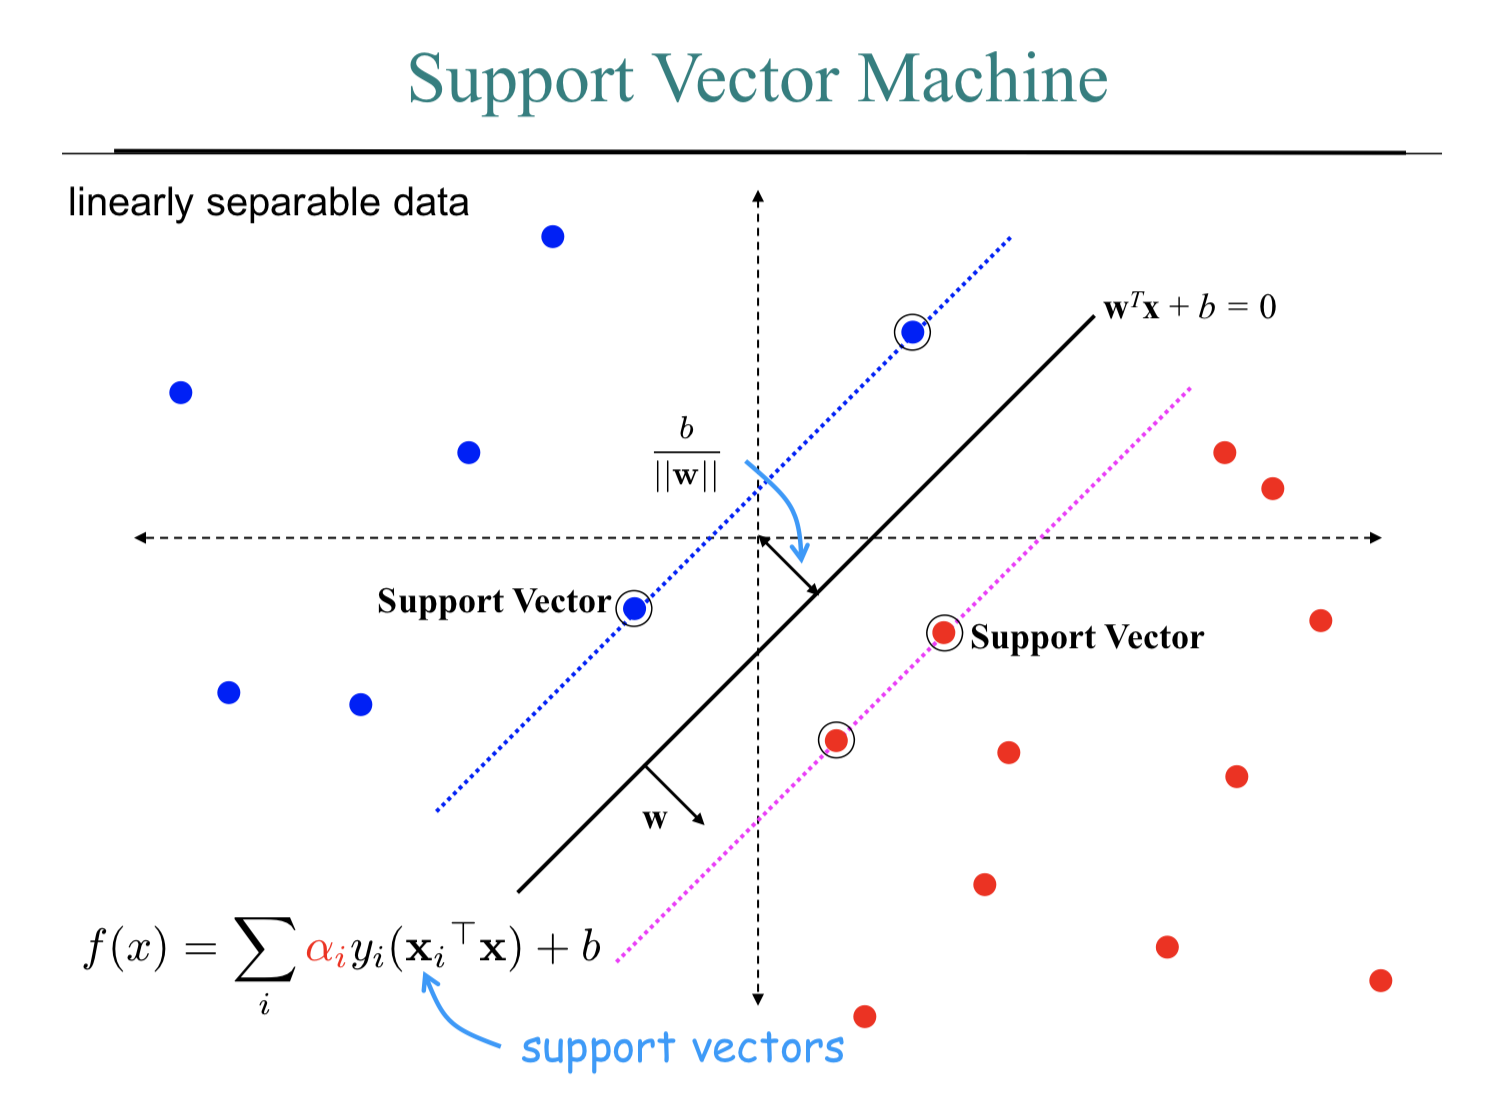
\includegraphics[width=0.9\textwidth]{img/svm_pic.png}
\caption{SVM classification}
\end{figure}

\subsection{Hard margin}
The simplest flavour of the linear SVM is referred to as the `hard margin'. In this setting, the hyperplane is chosen to maximise the distance between the nearest datasets.

Let $\mathbf{x}^+$ and $\mathbf{x}^-$ be two of the possible support vectors from each class. From the definition of the decision boundary, there is a degree of freedom in the scale of the weights $\mathbf{w}$. As a result, we normalise the weights to ensure
\begin{align}
\mathbf{w}^\top\mathbf{x}^+=+1\\
\mathbf{w}^\top\mathbf{x}^-=-1
\end{align}
Having performed this normalisation, the length of the margin, $M$, can then be expressed in terms of the norm of the weights
\begin{align}
M &=\hat{\mathbf{w}}^\top(\mathbf{x}^+-\mathbf{x}^-)\\
&=\frac{\mathbf{w}^\top(\mathbf{x}^+-\mathbf{x}^-)}{|\mathbf{w}|}\\
&=\frac{2}{|\mathbf{w}|}
\end{align}
where $\hat{x}$ denotes the vector $x$ with unit length. As a result, maximising the margin $M$ is equivalent to the following optimisation
\begin{align}
\mathbf{w}^*=\argmin_\mathbf{w} |\mathbf{w}|\qquad s.t. \qquad y_i(\mathbf{w}^\top\mathbf{x}_i+b)\ge1
\end{align}


\subsection{Soft margin}
When data is not linearly separable it can often be more beneficial to allow points from each class to encroach on the margin. In some cases this may mean the training points are such that the resulting hyperplane correctly classifies them (though they are closer to the hyperplane than the support vectors) though in other cases it may mean the fitted hyperplane would misclassify one or more points in the training set. The number of misclassifications will be seen to depend on a hyperparameter of the algorithm.

Figure \ref{fig:svm_slack} provides an example of binary classification where some subset of the training data is allowed to be closer to the decision boundary than the support vectors used to define it. In such a setting, where training data enters into the margin, `slack variables' $\xi_i$ are introduced to measure how far into the margin each violation is.

For the weights normalised as above, then the width of the margin is by definition equal to $\frac{2}{|\mathbf{w}|}$. As a result, for $\xi_i \in [0,1]$ the training point $\mathbf{x}_i$ is correctly classified though violating the margin boundary and for $\xi_i>1$ the point is misclassified. In this regard, `large' values of the slack variables constitute either more margin violations or more misclassifications.

Capturing this in an optimisation, for some regularisation parameter $C$ we are able to formalise this as
\begin{align}
\mathbf{w}^*=\argmin_\mathbf{w} |\mathbf{w} |+ C\sum_{i=1}^N\xi_i\\
 s.t. \qquad y_i(\mathbf{w}^\top\mathbf{x}_i+b)\ge1-\xi_i
\end{align}
where large $C$ implies heavier penalisation of the slack variables and so a `harder' margin.

Equivalently, the above optimisation may be restated in terms of the more familiar expression for $\varphi$-risk

\begin{align}
\mathbf{w}^*=\argmin_\mathbf{w} |\mathbf{w} |+ C\sum_{i=1}^N\max(0,1-y_if(\mathbf{x}_i))
\end{align}

Note, in particular that the implied cost function can be differentiated w.r.t. each component of $\mathbf{w}$ except at discontinuities implied by the hinge loss.

\begin{figure}
\center
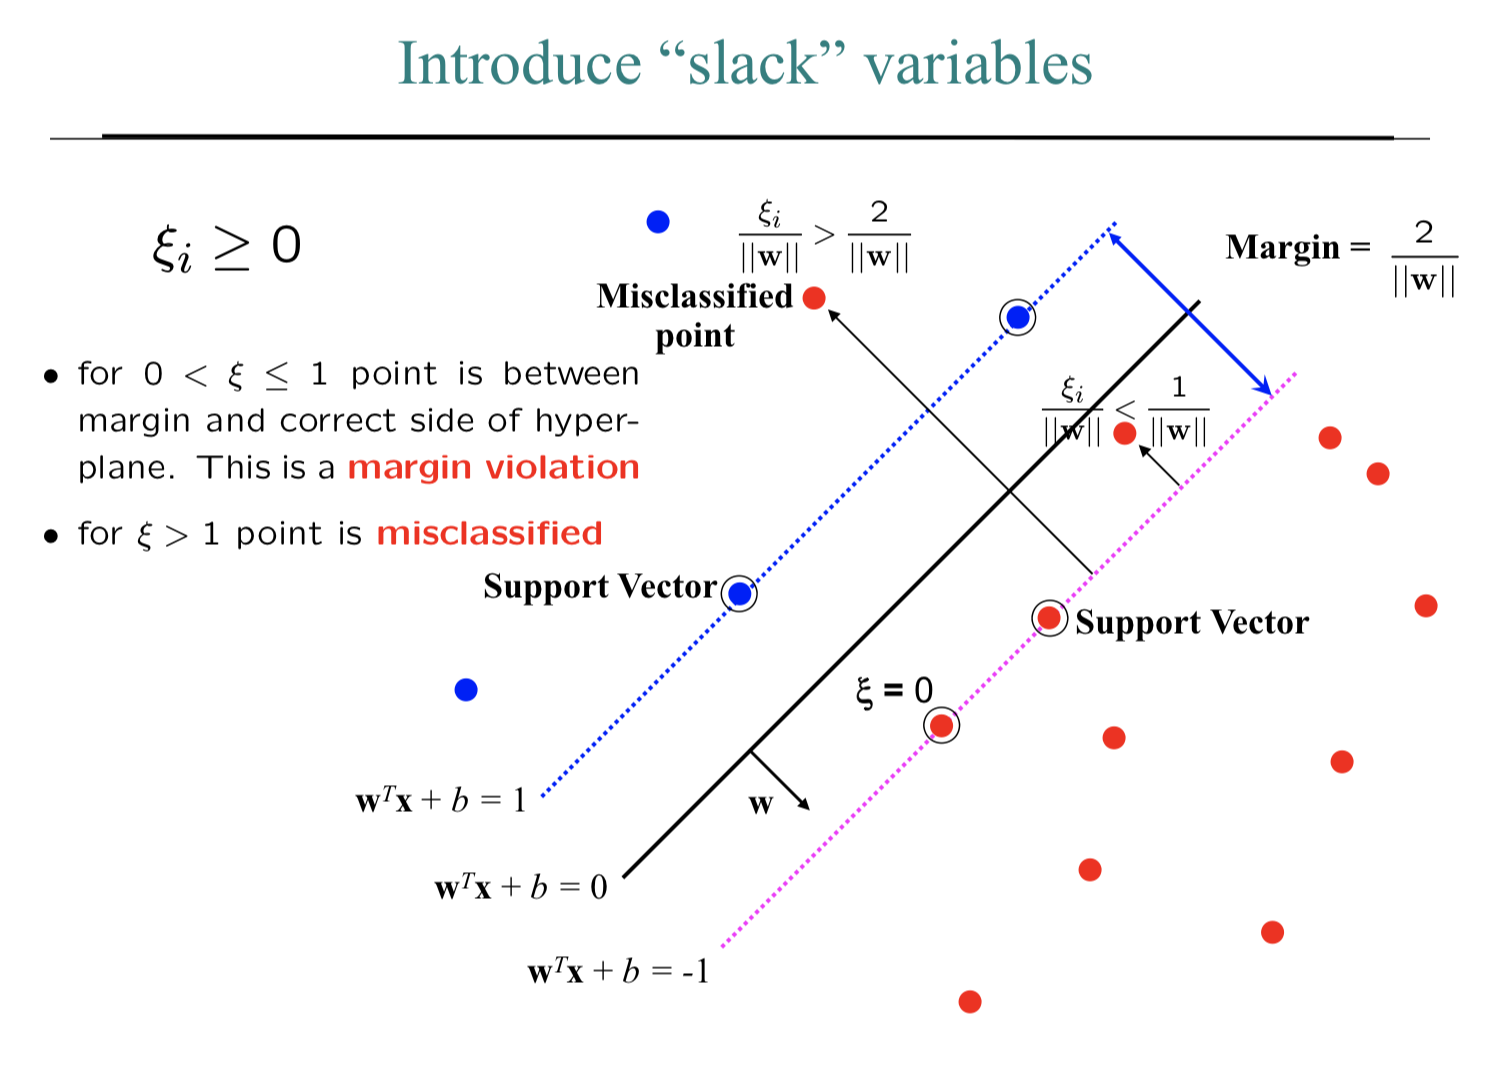
\includegraphics[width=0.9\textwidth]{img/slack_var.png}
\caption{SVM classification with slack variables}
\label{fig:svm_slack}
\end{figure}
%\subsection{Dual formulation and the `kernel trick'}


%\input{11_Kernels_SVM_written_by_Lawrence}

\section{Reproducing Kernel Hilbert Spaces}

Motivated by the above introduction to SVMs under linear classifiers, the following will extend this to the case where linear separation of the data will not yield a strong classifier. The solution to this problem can be found by introducing feature maps $\Phi\colon \mathcal{X} \rightarrow \mathcal{H}$, where $\mathcal{H}$ is an appropriate Hilbert space. With the right choice of $\mathcal{H}$ the features $\Phi(x_i), i=1, \ldots, n$ can then be separated using support vector machines. We will conclude with a coverage of generalisation bounds, aiming to analyse the trade-off between overfitting a flexible class of functions to a small amount of data and underfitting a smaller class of functions to a larger amount of data.

As will be seen, the choice of Hilbert space used for the classification problem can be constructed through the definition of positive semi-definite kernel (defined explicitly below).  The following defines such kernels and explore some of its properties. Subsequently the construction of the relevant Hilbert space over which the classification problem for SVMs can be performed is constructed.

\begin{definition}
A function $k\colon \mathcal{X}\times \mathcal{X} \rightarrow \mathbb{R}$ is called a \emph{positive symmetric definite kernel} (PSD kernel) if
\begin{itemize}
	\item[i)] For all $x, y$, $$k(x, y)=k(y, x);$$
	\item[ii)] For any finite collection $x_1, \ldots, x_n \in \mathcal{X}$, the matrix defined by
	\begin{equation}
		\mathbf{K} := (k_{i,j})_{i,j} := (k(x_i, x_j))_{i,j}
	\end{equation}
	is positive \underline{semi}-definite, that is, for all $n\in \mathbb{N}$, all $x_1, \ldots, x_n$ and any $a_1, \ldots, a_n \in \mathbb{R}$
	\begin{equation*}
	 \sum_{i=1}^n\sum_{j=1}^n a_ia_j k(x_i, x_j) = a^T\mathbf{K}a \geq 0.
	\end{equation*}
\end{itemize}
\end{definition}

\begin{example}[Kernels]
\begin{itemize}
	\item[a)] Let $\X = \R^d$ and $k(x,y) = x^Ty$ the usual inner product. Then $k$ is a PSD since for any $a_1, \ldots, a_n \in \R$
	\begin{equation*}
		\sum_{i,j} a_ia_j x_i^Tx_j = \sum_{i,j} (a_ix_i)^T(a_j x_j) = (\sum_i a_ix_i)^T(\sum_j a_j x_j) = \left\|\sum_i a_i x_i \right\|^2 \geq 0.
	\end{equation*}
	\item[b)] \emph{(Without proof)} The Gaussian kernel (or Gaussian RBF) $$k(x, y) =  \exp\left(-\frac{\|x - y\|^2}{\gamma}\right).$$
	The Gaussian kernel is governed by some parameter $\gamma >0$, which can be interpreted in the following way: consider the feature map $\Phi \colon x \mapsto k(\cdot, x)$ for some observations $x_1, \ldots, x_n$. For $\gamma$ small the features $\Phi(x_1),\ldots, \Phi(x_n)$ are almost independent, whereas for $\gamma$ large the features are almost parallel.
\end{itemize}
\end{example}

\begin{definition}
Let $W$ denote a Hilbert space of real valued functions $f\colon \mathcal{X} \rightarrow \mathbb{R}$. A function $k\colon \mathcal{X}\times \mathcal{X} \rightarrow \mathbb{R}$ is called a \emph{reproducing kernel} for $W$ if
\begin{itemize}
	\item[i)] For all $x \in \mathcal{X}$: $k(x, \cdot) \in W$;
	\item[ii)] for all $x \in \mathcal{X}$ and $f \in W$:
	\begin{equation*}
		f(x) = \langle f, k(x, \cdot) \rangle_W \quad \text{(reproduction).}
	\end{equation*}
\end{itemize}
Hilbert spaces for which such a $k$ exists are called \emph{reproducing kernel Hilbert spaces (RKHS).}
\end{definition}
In the literature RKHS are sometimes defined as a Hilbert space of real valued functions with the property that the point evaluation functions $\delta_x \colon  f \mapsto f(x)$ are continuous for all $x \in \X$. It is not difficult--using Cauchy-Schwarz and the Riesz representation theorem--to establish that both definitions are equivalent. In fact, the continuity of evaluation functions in reproducing kernel Hilbert spaces follows from the following lemma.
\begin{lemma}\label{lem:kernel}
A kernel $k$ has the following properties
\begin{align*}
	\langle k(x, \cdot), k(y, \cdot) \rangle_W = k(x, y)
	\intertext{and}
	\sup_{x\in{\mathcal{X}}} |f(x)| \leq \|f\|_W \sup_{x\in\mathcal{X}} \sqrt{k(x, x)}.
\end{align*}
\end{lemma}

\begin{proof}
The first part follows from reproduction
\begin{equation*}
	\langle f, k(x, \cdot) \rangle_W = f(x)
\end{equation*}
using $f(x) = k(y, x)$. Also by reproduction and Cauchy-Schwarz
\begin{align*}
	\sup_{x\in\X} f(x)^2 = \sup_{x\in\X} \langle f, k(x, \cdot) \rangle_W^2 \leq \sup_{x\in\X}\|f\|_W^2\|k(x, \cdot\|_W^2.
\end{align*}
By the first part $\|k(x, \cdot )\|_W^2 = \langle k(x, \cdot), k(x, \cdot) \rangle_W = k(x, x)$ so the result follows.
\end{proof}

Based on this lemma we can establish a further characterisation which is especially useful in practice (see Example c).
\begin{proposition}
If $k\colon \X \times \X$ is a reproducing kernel for some Hilbert space $W$, then $k$ is a PSD kernel. Conversely let $k$ be a PSD kernel then $k$ is a reproducing kernel.
\end{proposition}
\begin{proof}
We show only the first part. Let $a_1, \ldots, a_n \in \R$, then
\begin{align*}
	\sum_{i,j} a_ia_j k(x_i, x_j) &= \sum_{i,j} a_ia_j \langle k(x_i, \cdot ), k(x_j, \cdot ) \rangle_W \\
	&= \left\langle \sum_{i} a_i  k(x_i, \cdot ), \sum_j a_jk(x_j, \cdot ) \right\rangle_W \\
	&= \left\| \sum_i a_i k(x_i, \cdot) \right\|_W^2 \geq 0.
\end{align*}
\end{proof}

The question that arises now is how to build a RKHS given a kernel. In the following we will give some examples how to build reproducing kernel Hilbert spaces from some kernel $k$.

\begin{example}[RKHS]
\begin{itemize}
	\item[a)] We start with a counter example. Consider the space $L^2([0, 1])$. Then the point evaluations $\delta_x: f \mapsto f(x)$ are not continuous, so $L^2([0, 1])$ cannot be a RKHS. (Note that elements of $L^2$ are only defined almost everywhere.)
	\item[b)] Denote $\varphi_1, \ldots, \varphi_n$ an orthonormal system in $L^2(\X)$. Then for arbitrary $a_k > 0, k \in \mathbb{N}$
	\begin{equation}
		k(x, y) := \sum_{j=1}^M a_j \varphi_j(x)\varphi_j(y)
	\end{equation}
	is a reproducing kernel for
	\begin{equation*}
		W := \mathrm{span}\left\{\varphi_1, \ldots, \varphi_n\right\}
	\end{equation*}
	equipped with inner product
	\begin{equation*}
		\langle f, g \rangle_W = \sum_{j=1}^M a_j^{-1} \langle f, \varphi_j \rangle_{L^2} \langle g, \varphi_j \rangle_{L^2}.
	\end{equation*}
	This follows for every $f \in W$ from
	\begin{align*}
		\langle f, k(x, \cdot ) \rangle_W &= \sum_{i=1}^n a_i^{-1} \langle f, \varphi_i \rangle_{L^2} \langle k(x, \cdot ), \varphi_i \rangle_{L^2} \\
		& = \sum_{i=1}^n a_i^{-1} \langle f, \varphi_i \rangle_{L^2} \langle \sum_{j=1}^n a_j \varphi_j(x)\varphi_j(\cdot), \varphi_i \rangle_{L^2} \\
		& = \sum_{i=1}^n a_i^{-1} \langle f, \varphi_i \rangle_{L^2} \sum_{j=1}^n a_j \varphi_j(x)\langle \varphi_j, \varphi_i \rangle_{L^2} \\
		& = \sum_{i=1}^n a_i^{-1} \langle f, \varphi_i \rangle_{L^2} \varphi_i(x) a_i \\
		& = \sum_{i=1}^n \langle f, \varphi_i \rangle_{L^2} \varphi_i(x) = f(x). \\
	\end{align*}
	Note that this construction can be extended to infinite series as long as $k(x, y)$ is well defined. Mercer's theorem here establishes a connection to self-adjoint integral operators.
	\item[c)] Given a PSD kernel, consider
	\begin{equation*}
			W = \mathrm{span}\left\{k(x_1, \cdot), \ldots, k(x_n, \cdot)\right\}
	\end{equation*}
	for pairwise different $x_1, \ldots, x_n \in \X$. Note for $f, g \in W$ we can write
	\begin{equation*}
		f(x) = \sum_{i=1}^n a_i k(x_i, x), \quad g(x) = \sum_{i=1}^n b_i k(x_i, x).
	\end{equation*}
	$W$ is a RKHS with inner product
	\begin{equation*}
		\langle f, g \rangle_W = \sum_{i=1}^n\sum_{j=1}^n a_i b_i k(x_i, x_j) = a^T\mathbf{K}b.
	\end{equation*}
	Then
	\begin{equation*}
		f(x_j) = \sum_{i=1}^n a_i k(x_i, x_j) = \langle f, k(x_j, \cdot ) \rangle_W
	\end{equation*}
	This way is popular in practice since we can construct an RKHS by just using the PSD kernel $k$ and the datapoints $x_1, \ldots, x_n$. We can, for example, use the Gaussian radial kernel as introduced above. Then $W$ consists of linear combinations of Gaussian bell curves. %If we use $k(x, y) = \langle x, y \rangle_{\R^d}$ this leads to the space of
	\item[d)] (optional) Denote $W = \{f \colon [0, 1] \rightarrow \mathbb{R} : f(0) = 0, \int_0^1 f'(x)^2 dx < \infty \}$, where $f'$ is assumed to exist in the weak sense. $W$ is a RKHS with $\langle f, g \rangle_W = \langle f', g' \rangle$ and reproducing kernel $k(x, y) = \min\{x, y\}$ since
	\begin{equation*}
		\langle f, k(x, \cdot) \rangle_W = \int_0^1 f'(y)\frac{\partial }{\partial y} \min\{x, y\}dy = \int_0^1 f'(y)1_{\{y \leq x\}} dy = f(x).
	\end{equation*}
	$W$ is known more broadly as a \emph{Cameron-Martin-Space}, serving an important role in the analysis of stochastic processes. Here, $k(x, y) = \E\left[B_xB_y \right] = \min\{x, y\}$ is the covariance function of Brownian motion $(B_t)_{t \in [0, 1]}$. Further
	\begin{equation*}
		\E\left[\langle f, B \rangle_W \langle g, B  \rangle_W \right] := \E\left[\int f' dB \int g' dB \right] = \langle f, g \rangle_W.
	\end{equation*}
\end{itemize}
\end{example}

\begin{theorem}[Representer Theorem]\label{theo:representer}
Let $W$ denote a RKHS with PSD $k$ and let $G$ denote an arbitrary function. Then
\begin{align*}
	\min_{f\in W, \|f|\leq \lambda} G\left(f(x_1), \ldots, G(f(x_n))\right) &= \min_{f\in V, \|f|\leq \lambda} G\left(f(x_1), \ldots, G(f(x_n))\right)
\end{align*}
where we define
\begin{equation*}
	V := \mathrm{span}\left\{k(x_1, \cdot), \ldots, k(x_n, \cdot)\right\}.
\end{equation*}
Moreover, writing $f \in V$ as $f = f_a = \sum_{i=1}^n a_i k(x_i, \cdot), a \in \R^d$ we get
\begin{equation*}
	\min_{f\in W, \|f|\leq \lambda} G\left(f(x_1), \ldots, G(f(x_n))\right) = \min_{a\in \R^d, a^T\mathbf{K}a \leq \lambda^2} G\left(f_a(x_1), \ldots, G(f_a(x_n))\right).
\end{equation*}
\end{theorem}
\begin{proof}
Denote $V^\perp := \{x \in W : \langle u, v \rangle_W = 0 \quad \forall v \in V\}$ the orthogonal complement of $V$ in $W$. Then any $f\in W$ can be decomposed in $f = v + u$ with $v \in V$ and $u\in V^\perp$. Pythagoras yields
\begin{equation*}
	\|f\|_W^2 = \|v\|_W^2 + \|u\|_W^2.
\end{equation*}
Moreover, since by definition $k(x_i, \cdot) \in V$ for any $i$, we have
\begin{equation*}
	u(x_i) = \langle u, k(x_i, \cdot) \rangle_W = 0.
\end{equation*}
Hence, $f(x_i) = v(x_i)$ and $u$ does not contribute to the constraint
\begin{equation*}
	\min_{f\in W, \|v|^2+\|u|^2\leq \lambda^2} G\left(f(x_1), \ldots, G(f(x_n))\right) = \min_{v\in W, \|v|^2\leq \lambda^2} G\left(v(x_1), \ldots, G(v(x_n))\right).
\end{equation*}
This shows the first part. The second part can be seen as follows. Note that by restricting our search for the minimum to $f \in V$ we can write $f_a$ as $f_a = \sum_{i=1}^n a_i k(x_i, \cdot)$. Hence,
\begin{align*}
	\|f_a\|^2 &= \langle f_a, f_a \rangle \\
						&= \left\langle \sum_{i=1}^n a_i k(x_i, \cdot),\sum_{j=1}^n a_j k(x_j, \cdot)\right\rangle \\
						&= \sum_{i=1}^n\sum_{j=1}^n a_i a_j \langle k(x_i, \cdot),k(x_j, \cdot) \rangle \\
						&= \sum_{i=1}^n\sum_{j=1}^n a_i a_j k(x_i,x_j) \\
						&= a^T\mathbf{K}a.
\end{align*}
This concludes the second part of the proof.
\end{proof}


\section{SVMs and RKHS}

We we will now apply these results to classification and support vector machines. Recall, we want to find the classifier (some $f$ in a pre-determined class of functions) that minimises the empirical $\varphi$-risk, where $\varphi$ denotes a convex relaxation of the $0-1$ loss. In the following, we will confine our attention to the popular hinge loss, $\varphi(z) = (1 + z)_+$.

\begin{definition}
Let $k$ denote a reproducing kernel and denote $W$ a RKHS. For $\lambda > 0$ set
\begin{equation}\label{eq:svm}
	\hat{f}_\mathrm{SVM} := \argmin_{f \in W: \|f\|_W \leq \lambda} \frac{1}{n}\sum_{i = 1}^n \left(1 - Y_i f(X_i)\right)_+,
\end{equation}
where we used the hinge loss.
\end{definition}

We can apply \autoref{theo:representer} to rewrite \eqref{eq:svm} as
\begin{align*}
	\hat{f}_\mathrm{SVM} &= \argmin_{f \in W: \|f\|_W \leq \lambda} \frac{1}{n}\sum_{i = 1}^n \left(1 - Y_i f(X_i)\right)_+ \\
											 &= \argmin_{a \in \R^n: a^T\mathbf{K}a \leq \lambda^2} \frac{1}{n}\sum_{i = 1}^n \left(1 - Y_i \sum_{j=1}^n a_j k(X_i, X_j)\right)_+ \\
											 &= \argmin_{a \in \R^n} \left\{\frac{1}{n}\sum_{i = 1}^n \left(1 - Y_i \sum_{j=1}^n a_j k(X_i, X_j)\right)_+ + \lambda' \sum_{i=1}^n\sum_{j=1}^n a_ia_j K(X_i, X_j) \right\}
\end{align*}
where we used Lagrange duality in the last line for some suitable $\lambda'$.

For further interpretation we can rewrite the minimization problem again
\begin{align*}
	\left(\hat{f}_\mathrm{SVM}, \hat{\xi} \right) &= \argmin_{f \in W, \xi \in \R_{\geq 0}^n, Y_if(X_i) \geq 1 - \xi_i} \left\{\frac{1}{n}\sum_{i=1}^n \xi_i + \lambda'\|f\|_W^2\right\} \\
	&=\argmin_{a\in\R^n, \xi \in \R_{\geq 0}^n, Y_i\sum_{j=1}^n a_j k(X_i, X_j) \geq 1 - \xi_i} \left\{\frac{1}{n}\sum_{i=1}^n \xi_i + \lambda'a^T\mathbf{K}a\right\}.
\end{align*}
Now, if all $(X_i, Y_i)$ are classified correctly with at least $Y_if(X_i) \geq 1$, then $\hat{\xi} = 0$ and the we only minimize over $$a^T\mathbf{K}a = \sum_ia_i \sum_j a_j k(x_i, x_j)=\sum_i a_i f(x_i)_.$$


\section{Generalisation bounds}
The following inequality aims to provide some insight into the increase in expected empirical risk under the SVM classifier above the $\varphi$-risk, $\inf_{\|f\|_W\leq \lambda} R_\varphi(f)$.

\begin{theorem}[Expected Excess Risk]\label{eq:excess_risk}
Denote the (hard) SVM-classifier as $\hat{h}_n^\mathrm{SVM}$ based on the hinge-loss in a kernel RKHS $W$ with $\sup_{x \in \mathcal{X}} k(x, x) < \infty$. Then the following bound holds for the expected risk and some radius $\lambda> 0$
\begin{equation*}
	\E\left[R(\hat{h}_n^\mathrm{SVM})\right] \leq \inf_{\|f\|_W\leq \lambda} R_\varphi(f) + 8 \lambda\E\left[k(X, X)\right]^{1/2}n^{-1/2}
\end{equation*}
\end{theorem}

We will need the following contraction principle by Ledoux and Talagrand, which we will just state as a lemma.
\begin{lemma}[Contraction principle]\label{lemma:contraction}
For a map $\psi\colon [-1, 1] \rightarrow \R$ with $|\psi(x) - \psi(y)|\leq | x- y|$ and $\psi(0) = 0$ we have for any family of measurable function $\mathcal{G} = \{g: \mathcal{X} \times \{-1, +1\} \rightarrow [-1, 1]\}$
\begin{equation*}
	\E\left[\sup_{g\in \mathcal{G}}\left|\frac{1}{n}\sum_{i=1}^n\sigma_i\psi(g(X_i, Y_i))\right|\right] \leq 2\E\left[\sup_{g\in \mathcal{G}}\left|\frac{1}{n}\sum_{i=1}^n\sigma_ig(X_i, Y_i)\right|\right].
\end{equation*}
\end{lemma}

\begin{proof}[Proof of \autoref{eq:excess_risk}]
Denote $X, Y$ a sample from the joint data distribution $P^{X, Y}$ independent of $\hat{f}_n^\mathrm{SVM}$, i.e. independent of all random variables used for classification. For the hinge loss $\varphi(x) = \max\{0, 1 + x\}$ we get
\begin{align*}
	R(\hat{h}_n^\mathrm{SVM}) &= \mathbb{P}^{X, Y}(-Y\hat{f}_n^\mathrm{SVM}(X) > 0) \\ 
	&\leq \E^{X, Y}\left[\max\left\{0, 1- Y\hat{f}_n^\mathrm{SVM}(X) \right\} \right] \\
	& = R_\varphi(\hat{f}_n^\mathrm{SVM})
\end{align*}
We can estimate
\begin{equation*}
	R_\varphi(\hat{f}_n^\mathrm{SVM}) - \inf_{\|f\|_W \leq \lambda} \leq 2 \sup_{\|f\|_W\leq \lambda} \left|R_{\varphi,n}(f) - R_\varphi(f)\right|.
\end{equation*}
Hence the proof is complete as soon as we can show
\begin{equation*}
	\E\left[\sup_{\|f\|_W\leq \lambda} \left|R_{\varphi,n}(f) - R_\varphi(f)\right|\right] \leq 4\lambda \sqrt{\frac{\E\left[k(X, X)\right]}{n}}.
\end{equation*}
By symmetrisation and a contraction argument we can upperbound the left-hand-side by the Rademacher complexity. To show this we introduce a \emph{ghost sample} $(X_i', Y_i'), i=1, \ldots,n$ which is an independent copy of the original sample following the same distribution. Denoting $\mathcal{D}$ the $\sigma$-algebra spanned by $(X_i, Y_i)_{i=1, \ldots, n}$ we get by Jensen's inequality
\begin{align*}
	\E\left[\sup_{\|f\|_W\leq \lambda} \left|R_{\varphi,n}(f) - R_\varphi(f)\right|\right] &\leq \E\left[\sup_{\|f\|_W\leq \lambda} \left|\frac{1}{n}\sum_{i=1}^n\left(\varphi(-Y_if(X_i)) - \E\left[\varphi(-Y_i'f(X_i'))\right]\right)\right|\right] \\
	& \leq \E\left[\sup_{\|f\|_W\leq \lambda} \left|\frac{1}{n}\sum_{i=1}^n\left(\varphi(-Y_if(X_i)) - \E\left[\varphi(-Y_i'f(X_i'))\mid \mathcal{D}\right]\right)\right|\right] \\
	& \leq \E\left[\sup_{\|f\|_W\leq \lambda} \left|\E\left[\frac{1}{n}\sum_{i=1}^n\varphi(-Y_if(X_i)) - \varphi(-Y_i'f(X_i'))\mid \mathcal{D}\right]\right|\right] \\
	& \leq \E\left[\E\left[\sup_{\|f\|_W\leq \lambda} \left|\frac{1}{n}\sum_{i=1}^n\varphi(-Y_if(X_i)) - \varphi(-Y_i'f(X_i'))\right|\mid \mathcal{D}\right]\right].
\end{align*}
Now, $\pm(\varphi(-Y_if(X_i)) - \varphi(-Y_i'f(X_i')))$ have the same distribution, so we can replace this quantity with $\sigma_i\varphi(-Y_if(X_i)) - \varphi(-Y_i'f(X_i'))$, where $(\sigma_i)_{i\in \mathbb{N}}$ denotes the Rademacher process. We have
\begin{align*}
\E\left[\sup_{\|f\|_W\leq \lambda} \left|R_{\varphi,n}(f) - R_\varphi(f)\right|\right] &\leq \E\left[\sup_{\|f\|_W\leq \lambda} \left|\frac{1}{n}\sum_{i=1}^n\varphi(-Y_if(X_i)) - 1 + 1 - \varphi(-Y_i'f(X_i'))\right|\right] \\ 
&\leq 2\E\left[\sup_{\|f\|_W\leq \lambda} \left|\frac{1}{n}\sum_{i=1}^n\sigma_i\varphi(-Y_if(X_i)) - 1\right|\right]
\end{align*}
By noting that $\|f\|_W \leq \lambda$ we can conclude by \autoref{lem:kernel} that
$\|f\|_\infty \leq \lambda \sup_{x\in\X}k(x, x)^{1/2} =: L < \infty$ (by assumption).
Using the contraction argument by Ledoux and Talagrand \autoref{lemma:contraction} with the functions $\psi(z) = (\varphi(Lz) - 1)/L$ and $g(x, y) = -yf(x)/L \in [-1, 1]$ we get
\begin{equation*}
\E\left[\sup_{\|f\|_W\leq \lambda} \left|\frac{1}{n}\sum_{i=1}^n\sigma_i\frac{\varphi(-Y_if(X_i)) - 1}{L}\right|\right] \leq 2\E\left[\sup_{\|f\|_W\leq \lambda} \left|\frac{1}{n}\sum_{i=1}^n\sigma_i\frac{-Y_if(X_i)}{L}\right|\right].
\end{equation*}
The random variables $-Y_i\sigma_i$ are distributed as $\sigma_i$ which lets us conclude
\begin{equation*}
	\E\left[\sup_{\|f\|_W\leq \lambda} \left|R_{\varphi,n}(f) - R_\varphi(f)\right|\right] \leq 4 \E\left[\sup_{\|f\|_W\leq \lambda} \left|\frac{1}{n}\sum_{i=1}^n\sigma_if(X_i)\right|\right],
\end{equation*}
where the RHS denotes the Rademacher complexity $\mathcal{R}_n(\mathcal{F})$ of the set $\mathcal{F} = \{f \in W: \|f\|_W \leq \lambda\}$.
We bound the Rademacher complexity by using the structure of the reproducing Hilbert space. With Cauchy-Schwarz we obtain
\begin{align*}
	\mathcal{R}_n(\mathcal{F}) &= \E \left[\sup_{f \in \mathcal{F}} \left|\frac{1}{n}\sum_{i=1}^n \sigma_i f(X_i)  \right| \right] \\
	& = \frac{1}{n}\E \left[\sup_{f \in \mathcal{F}} \left|\sum_{i=1}^n \sigma_i \langle k(X_i, \cdot), f \rangle_W  \right| \right] \\
	& = \frac{1}{n} \E \left[\sup_{f \in \mathcal{F}} \left|\left\langle\sum_{i=1}^n \sigma_i  k(X_i, \cdot), f \right\rangle_W  \right| \right] \\ 
	& \leq \frac{1}{n} \E \left[\sup_{f \in \mathcal{F}} \sqrt{\|f\|_W^2 \left\|\sum_{i=1}^n \sigma_i k(X_i, \cdot) \right\|_W^2}\right] \\ 
	& \leq \frac{\lambda}{n}\E \left[\sqrt{\sum_{i=1}^n \sigma_i\sigma_j k(X_i, X_j)}\right].
\end{align*}
Now with Jensen
\begin{align*}
	\E \left[\sqrt{\sum_{i=1}^n \sigma_i\sigma_j k(X_i, X_j)}\right] &\leq  \sqrt{\E \left[\sum_{i=1}^n \sigma_i\sigma_j k(X_i, X_j)\right]} \\ 
	&\leq  \sqrt{\sum_{i=1}^n \E\left[k(X_i, X_j)\right] \E \left[\sigma_i\sigma_j \right]} \\ 
	&\leq  \sqrt{\sum_{i=1}^n\sum_{j=1}^n\E\left[k(X_i, X_i)\right] \delta_{ij}} \\
	&\leq \sqrt{n}\sqrt{\E\left[k(X, X)\right]}.
\end{align*}
This concludes the proof.
\end{proof}
As stated, the above theorem provides only the excess risk in expectation over the data. Further (and structurally similar) bounds exist bounding the excess risk in high probability. These can be found in the Rigolet lecture notes.

%!TEX root = optimization1718.tex

\chapter{AdaBoost}
\emph{Speaker: Adam Foster, 16/03/2018.}\\

In ensemble methods for machine learning we assume that
\begin{equation*}
	(W_1, Y_1), \dots, (W_n, Y_n)
\end{equation*}
are i.i.d. with $W_i \in \mathcal{W}$. For binary classification, we have $Y_i \in \{\pm 1\}$. We have access to a set $\mathcal{G}$ of base (also called weak) procedures
\begin{equation*}
	g: \mathcal{W} \to \{\pm 1\} \text{ for } g \in \mathcal{G}
\end{equation*}

The aim is to construct an aggregate of base procedures which solves the following optimization problem
\begin{align*}
	\begin{aligned}
		\min_f\quad   & \E \ell(f(W), Y) \\
		\text{subject to }\quad & f = \sum_{t=1}^T \alpha_t g_t \text{ with } \alpha_t \ge 0, g_t \in \mathcal{G} \text{ for } t=1, \dots, T.
	\end{aligned}
\end{align*}

As in Section~\ref{sec:intro}, $\ell$ is a loss functions typically of the form $\ell(z,y) = \varphi(-zy)$ for a given $\varphi:\R\rightarrow\R$. A natural loss function in the classification regime is the Zero-One loss
\begin{align*}
	\ell_{01}(f(w), y) &= \mathbf{1}[\text{sign}(f(w)) \ne y] \\
	\varphi_{01}(u)    &= \mathbf{1}[u \ge 0]
\end{align*}
but regrettably this is neither convex nor differentiable. In AdaBoost, we use the Exponential Loss
\begin{equation*}
	\varphi_\text{exp}(u) = \exp(u)
\end{equation*}
which is an upper bound on $\varphi_{01}$.

Since the distribution of $(W, Y)$ is unknown, we optimize the \textbf{empirical} loss
\begin{equation*}
	\E_n \ell(f(W), Y) = \frac{1}{n} \sum_{i=1}^n \ell(f(W_i), Y_i)
\end{equation*}


\section{The AdaBoost algorithm}
\label{sec:adaboost_derive}

AdaBoost is a recursive algorithm that greedily minimizes the empirical exponential loss, $\ell_\text{exp}$, at each step.

Suppose that $f_{t-1}$ is given. Greedy minimization means that we choose $\alpha_t$ and $g_t$ to minimize
\begin{equation*}
	\E_n \ell_\text{exp} [f_{t-1}(W) + \alpha_t g_t(W), Y] = \frac{1}{n} \sum_{i=1}^n \exp[-Y_i f_{t-1}(W_i)]\exp[-\alpha_t Y_i g_t(W_i)]
\end{equation*}
define the normalized weights $D_t(i) \propto \exp[-Y_i f_{t-1}(W_i)]$. The objective is then proportional to
\begin{align}
	\label{eq:adaboost_empirical_loss}
	&\sum_{i=1}^n D_t(i)\exp[-\alpha_t Y_i g_t(W_i)] = e^{-\alpha_t} + (e^{\alpha_t} - e^{-\alpha_t}) \sum_{i=1}^n D_t(i)\mathbf{1}[Y_i \ne g_t(W_i)]
\end{align}
Recall $\alpha_t \ge 0$, so $e^{\alpha_t} \ge e^{-\alpha_t}$. Thus we can first choose $g_t$ to minimize the weighted misclassification error
\begin{equation*}
	\varepsilon_t = \sum_{i=1}^n D_t(i)\mathbf{1}[Y_i \ne g_t(W_i)]
\end{equation*}
then the optimal $\alpha_t$ is simply
\begin{equation}
	\label{eq:adaboost_alpha_optim}
	\alpha_t = \tfrac{1}{2}\log \left(\frac{1 - \varepsilon_t}{\varepsilon_t}\right)
\end{equation}

We have just derived the following algorithm
\begin{algorithm}
%\scriptsize
\caption{AdaBoost}
   \begin{algorithmic}[1] \label{alg:adaboost}
   \STATE Let $f_0 \equiv 0$
   \STATE Let $D_1(i) = \tfrac{1}{n}$
   \FOR{$t = 1$ to $T$}
   	\STATE Choose $g_t \in \mathcal{G}$ to minimize the weighted misclassification error $\varepsilon_t = \sum_{i=1}^n D_t(i)\mathbf{1}[Y_i \ne g_t(W_i)]$
   	\STATE Let $\alpha_t = \tfrac{1}{2}\log \left(\frac{1 - \varepsilon_t}{\varepsilon_t}\right)$
    \STATE Let $f_t$ = $f_{t-1} + \alpha_t g_t$
    \STATE Reweight $D_{t+1}(i) \propto D_{t}(i)\exp(-\alpha_t Y_i g_t(W_i))$
   \ENDFOR
   \STATE Normalize $f = f_T/\sum_{t=1}^T \alpha_t$
\end{algorithmic}
\end{algorithm}

\subsection{Choice of \texorpdfstring{$\mathcal{G}$}{G}}
In classification, it is extremely common to choose the base procedures to be some form of decision tree. Two common cases are:
\begin{itemize}
	\item Decision stumps. For $\mathcal{W} = \R^k$, the $(i, c, s)$-decision stump assigns $+s$ to $\{w : w_i \ge c\}$ and $-s$ to the rest. (We need $s=\pm 1, 1 \le i \le k, c \in \R$.)
	\item Decision trees. For $\mathcal{W} = \R^k$, decision trees recursively split the input space into a number of (hyper)rectangles and assign $+1$ or $-1$ to each rectangle. They are a generalization of decision stumps.
\end{itemize}

\subsection{Benefits of exponential loss}
A useful property of the Exponential Loss $\ell_\text{exp}$ is that it has the same population minimizer as $\ell_{01}$.

To see this, first apply the Law of Total Expectation
\begin{equation*}
	\E[\exp(-Yf(W))] = \E[\E[\exp(-Yf(W))|W]].
\end{equation*}
It suffices to minimize the conditional expectation pointwise
\begin{equation*}
	\E[\exp(-Yf(w))] = e^{-f(w)}\Prob(Y=1|W=w) + e^{f(w)}\Prob(Y=-1|W=w)
\end{equation*}
we then differentiate
\begin{equation*}
	\frac{\partial}{\partial f(w)} \left( e^{-f(w)}\Prob(Y=1|W=w) + e^{f(w)}\Prob(Y=-1|W=w) \right) = -e^{-f(w)}\Prob(Y=1|W=w) + e^{f(w)}\Prob(Y=-1|W=w)
\end{equation*}
and set the derivative equal to zero
\begin{align*}
	e^{-f^*(w)} \left( -\Prob(Y=1|W=w) + e^{2f^*(w)}\Prob(Y=-1|W=w) \right) = 0 \\
	f^*(w) = \tfrac{1}{2}\log \frac{\Prob(Y=1|W=w)}{\Prob(Y=-1|W=w)}
\end{align*}
which indeed gives the Zero-One minimizer.

\subsection{A geometric perspective on AdaBoost}
Recall the \textbf{Kullback-Leibler} (KL) divergence for distributions $p$ and $q$
\begin{equation*}
	KL(p, q) = \sum_{i=1}^n p(i) \log \frac{p(i)}{q(i)}
\end{equation*}
Let $u$ denote the uniform distribution on $1, \dots, n$. Consider the following optimization problem
\begin{align*}
	\begin{aligned}
		\min_p\quad   & KL(p, u)\\
		\text{subject to }\quad & p\in \Delta_n, \\
								& \sum_{i=1}^n p(i)Y_i g(W_i) = 0 \text{ for } g \in \mathcal{G}
	\end{aligned}
\end{align*}
The Lagrangian for this problem is
\begin{equation*}
	L(p, \alpha, \lambda) = \sum_{i=1}^n p(i) \log (np(i)) + \sum_{g \in \mathcal{G}} \alpha_g \left( \sum_{i=1}^n p(i)Y_i g(W_i) \right) + \lambda \left(\sum_{i=1}^n p(i) - 1\right)
\end{equation*}
(we have ignored the non-negativity constraints but it turns out we get them for free).

We differentiate $L$ w.r.t. $p(i)$
\begin{equation*}
	\frac{\partial L}{\partial p(i)} = \log(np(i)) + 1 + \sum_{g \in \mathcal{G}} \alpha_g Y_i g(W_i) + \lambda
\end{equation*}
and solve equal to 0
\begin{equation*}
	p(i) = \exp \left( - \sum_{g \in \mathcal{G}} \alpha_g Y_i g(W_i) \right)/Z
\end{equation*}
where $Z$ is a normalization constant.
The Lagrangian dual function is
\begin{equation*}
	g(\alpha, \lambda) = \log n - \log Z = \log n - \log \sum_{i=1}^n \exp \left( - \sum_{g \in \mathcal{G}} \alpha_g Y_i f(W_i) \right)
\end{equation*}
and the dual problem $\max_{\alpha, \lambda} g(\alpha, \lambda)$ is equivalent to
\begin{equation*}
	\min_\alpha \frac{1}{n}\sum_{i=1}^n \exp\left( - Y_i \sum_{g \in \mathcal{G}} \alpha_g g(W_i)\right)
\end{equation*}
which is the AdaBoost objective.

\section{Weak learning implies strong learning}
The set $\mathcal{G}$ of base procedures must have sufficient flexibility to give an edge over random guessing. More formally
\begin{definition}[Weak learners of parameter $\gamma$]
Set $\mathcal{G}$ is a family of \textbf{$\gamma$-weak learners} if for every distribution on $(W, Y)$ there exists $g \in \mathcal{G}$ such that
\begin{equation*}
	\Prob_{(W, Y)}[Yg(W) \le 0] \le \frac{1 - \gamma}{2}
\end{equation*}
\end{definition}

With this definition, we can begin a theoretical analysis of AdaBoost.

\begin{theorem}[AdaBoost with $\gamma$-weak learners]
The optimized empirical exponential loss of AdaBoost is
\begin{equation*}
	\prod_{t=1}^T 2 \sqrt{\varepsilon_t (1 - \varepsilon_t)}.
\end{equation*}
Suppose now that $\exists \gamma > 0$ such that $\mathcal{G}$ is a family of $\gamma$-weak learners. Then the empirical misclassification rate decreases to zero at the following exponential rate
\begin{equation*}
	\Prob_n [Yf(W) \le 0] \le (1 - \gamma^2)^{T/2}
\end{equation*}
and equals zero after at most $2\log n/\gamma^2$ iterations.

\begin{proof}
From equation~\eqref{eq:adaboost_empirical_loss} taking $t=T$ we first note that the constant of proportionality is $\frac{1}{n}\sum D_T(i)(W_i) = \E_n [\exp(-Yf_{T-1}(W))]$. Thus,
\begin{equation*}
	\E_n[\exp(-Yf_T(W)] = \left( e^{-\alpha_T} + \varepsilon_T(e^{\alpha_T} - e^{-\alpha_T}) \right) \E_n [\exp(-Yf_{T-1}(W))] \\
\end{equation*}
Using equation~\eqref{eq:adaboost_alpha_optim} we have $e^{\pm \alpha_T} = \left(\frac{1 - \varepsilon_T}{\varepsilon_T}\right)^{\pm 1/2}$, giving
\begin{align*}
	\E_n[\exp(-Yf_T(W)] &= 2\sqrt{\varepsilon_T (1-\varepsilon_T)} \E_n [\exp(-Yf_{T-1}(W))] \\
	&= \prod_{t=1}^T 2\sqrt{\varepsilon_t (1-\varepsilon_t)}
\end{align*}

Now suppose $\mathcal{G}$ is a family of $\gamma$-weak learners. Then (considering the empirical law on $(W, Y)$ in the definition of weak learners) we must have each $\varepsilon_t \le \frac{1 - \gamma}{2}$, since the choice of $g_t$ is optimal. Hence $2\sqrt{\varepsilon_t(1 - \varepsilon_t)} \le \sqrt{1 - \gamma^2}$

Finally, since $\varphi_\text{exp} \ge \varphi_{01}$, we have
\begin{align*}
	\Prob_n(Yf_T(W) \le 0) &\le \prod_{t=1}^T 2\sqrt{\varepsilon_t (1-\varepsilon_t)} \\
	&\le (1 - \gamma^2)^{T/2}
\end{align*}
as claimed.

Now, after $T = 2\log n/\gamma^2$ iterations, we have $(1 - \gamma^2)^{T/2} < e^{-\gamma^2 T/2} = 1/n$. But $\Prob _n(Yf_T(W))$ takes a minimum positive value $1/n$ and hence must be $0$.

\end{proof}
\end{theorem}


\section{Generalizations of AdaBoost}
AdaBoost can be generalized in a number of ways. Within the realm of classification, we can consider new loss functions like the logistic loss $\varphi(u) = \log_2 (1+ \exp(u))$. We can extend AdaBoost to multi-class classification. One way to do this is to let $Y \in \R^k$ with one component equal to $1$ and the others equal to $-1/(k-1)$. The Exponential Loss function becomes $\ell_\text{exp}(z, y) = \exp(-y^T z)$. The multi-class AdaBoost algorithm can then be derived exactly as in Section~\ref{sec:adaboost_derive}.

Boosting is also applicable to regression, where $Y \in \R$. In this context, one typically uses the least-squares loss $\ell(z, y) = (z - y)^2$. In the regression context, the possible choices for $\mathcal{G}$ become much larger. For instance:
\begin{itemize}
	\item Decision trees. Like classification trees, regression trees split the space recursively into rectangles and assign a real number to each rectangle.
	\item Single-hidden-layer neural networks. These take as output $\sigma(b + \langle x, W \rangle )$ where $\sigma$ is a nonlinear function, $b \in \R, x \in \mathcal{W}$.
	\item Wavelets.
	\item Regression splines.
	\item Reproducing kernel Hilbert spaces (RHKS). If $k: \mathcal{W} \times \mathcal{W} \to \R$ is a positive definite kernel, we may take $\mathcal{G}$ as the set $\{k(\cdot, w): w \in A\}$ where $A \subseteq \mathcal{W}$ is a collection of points
\end{itemize}
In the last three cases, suitable choices of $\mathcal{G}$ ensure that $\text{span}(\mathcal{G})$ consists of all (appropriate) real functions on $\mathcal{W}$.

\subsection{Boosting as variational gradient descent}
(This section is based on \cite{mason2000boosting}) \\
We can phrase the optimization problem that boosting targets as
\begin{equation}
	\min_{f \in \mathcal{F}} \; C(f)
\end{equation}
where $\mathcal{F} = \text{span}(\mathcal{G})$ consists of finite linear combinations of base procedures and $C(f) = \E_n \ell(f(W), Y)$ is the empirical loss. Under suitable conditions\footnote{for instance, if $\mathcal{F}$ is a Hilbert space and $C$ a differentiable functional}, one could approach this problem directly using gradient descent methods
\begin{equation*}
	f_t = f_{t-1} - \eta_t \partial C (f_{t-1}).
\end{equation*}
As an approximation, one could find
\begin{equation}
	\label{eq:functional_gradient_approx}
	g_t = \argmax_{g\in\mathcal{G}} \; -\langle \partial C(f_{t-1}), g \rangle
\end{equation}
and then
\begin{equation*}
	f_t = f_{t-1} + \alpha_t g_t
\end{equation*}
optimizing the non-negative coefficient $\alpha_t$ separately.

Whilst $\partial C(f_{t-1})$ may seem a daunting functional derivative, if we take the inner product
\begin{equation}
	\label{eq:boost_inner_prod}
	\langle f_1, f_2 \rangle = \frac{1}{n} \sum_{i=1}^n f_1(W_i)f_2(W_i)
\end{equation}
we have a more explicit form for the objective in \eqref{eq:functional_gradient_approx}
\begin{equation*}
	-\langle \partial C(f_{t-1}), g \rangle = -\frac{1}{n^2} \sum_{i=1}^n \frac{\partial \ell}{\partial z}(f_{t-1}(W_i), Y_i) \cdot g(W_i)
\end{equation*}

There are two interesting special cases. If $Y \in \{\pm 1\}$ and $\ell(z, y) = \varphi(-yz)$ then we have
\begin{align*}
	-\langle \partial C(f_{t-1}), g \rangle &= \frac{1}{n^2}\sum_{i=1}^n Y_i\varphi '(-Y_i f_{t-1}(W_i)) \cdot g(W_i) \\	
	&= \frac{1}{n^2}\sum_{i=1}^n \varphi ' (-Y_i f_{t-1}(W_i)) - \frac{2}{n^2} \sum_{i=1}^n \varphi ' (-Y_i f_{t-1}(W_i)) \mathbf{1}[Y_i \ne g(W_i)]
\end{align*}
assuming that $\varphi ' \le 0$ (sensible for classification) we see that $g$ is chosen to minimize the weighted empirical misclassification error.

If $Y \in \R$ and $\ell(z, y) = (z - y)^2$ then we have
\begin{align*}
	-\langle \partial C(f_{t-1}), g \rangle &= -\frac{1}{n^2}\sum_{i=1}^n 2(f_{t-1}(W_i) - Y_i) \cdot g(W_i)
\end{align*}
so $g$ is chosen to maximally counterbalance the residuals left by $f_{t-1}$.

The gradient perspective gives a recipe for producing a large number of Gradient Boosting algorithms as shown in Algorithm~\ref{alg:gradient_boosting}.

\begin{algorithm}
%\scriptsize
\caption{Gradient Boosting}
   \begin{algorithmic}[1] \label{alg:gradient_boosting}
   \STATE Let $f_0 \equiv 0$
   \FOR{$t = 1$ to $T$}
   	\STATE Choose $g_t \in \mathcal{G}$ to maximize $-\langle \partial C(f_{t-1}), g \rangle$, using the inner product of \eqref{eq:boost_inner_prod}
   	\STATE Choose $\alpha_t$ to minimize $C(f_{t-1} + \alpha_t g_t)$
    \STATE Let $f_t$ = $f_{t-1} + \alpha_t g_t$
   \ENDFOR
   \STATE Normalize $f = f_T/\sum_{t=1}^T \alpha_t$
\end{algorithmic}
\end{algorithm}





\section{Universal consistency of AdaBoost}

References:
\begin{itemize}
\item \verb|https://bcourses.berkeley.edu/courses/1409209/files/67384944|
\item \verb|http://statistics.berkeley.edu/sites/default/files/tech-reports/722.pdf|
\end{itemize}

We begin with a number of definitions. Recall the \textbf{classification risk}
\begin{equation*}
	R(f) = \Prob [f(W) \ne Y]
\end{equation*}
Let $R^* = \inf_f R(f)$ where the inf is taken over all classification rules\footnote{Note that classification rules are derived from training data. Classification rules generated from $n$ examples are therefore measurable w.r.t. the $\sigma$-algebra, $\Sigma_n$, generated by $(W_1, Y_1), \dots, (W_n, Y_n)$. The class considered here is all classification rules measurable under $\Sigma = \cup_n \Sigma_n$.} $f:\mathcal{W} \to \{\pm 1\}$.

A sequence $(f_n)$ of classification rules is \textbf{universally consistent} if
\begin{equation}
	\label{eq:universally_consistent}
	R(f_n) \to R^* \text{ a.s. as } n \to \infty
\end{equation}
for every distribution of $(W, Y)$.

A proof that AdaBoost is universally consistent can be found in (cite Bartlett).

\subsection{Classification calibration}
We want
\begin{equation*}
	R_\varphi (f_n) \to R^*_\varphi \implies R(f_n) \to R^*
\end{equation*}

\subsection{Sieves}
Let $\mathcal{F}_n$ be all classification rules obtainable with a sample of size $n$. Let $\bar{f}_n$ be the optimizer of $R_\varphi$ over this family. Then we want to prove that
\begin{equation}
	R_\varphi(\bar{f}_n) \to R^*
\end{equation}
and that the empirical risk and population risk get close
\begin{equation}
	|R_\varphi(\bar{f}_n) - R_{\varphi, n}(\bar{f}_n)| \to 0
\end{equation}

The concentration inequalities we seek to use require bounded $\varphi$. Hence, we clip them using $\pi_C$.

%!TEX root = optimization1718.tex

\chapter{Early Stopping for Kernel Boosting Algorithms}
\emph{Speaker: Fan Wu and Tomas Vaskevicius}\\


\section{Introduction}
Overfitting is a problem occurring in many models. Especially non-parametric models,
which offer great flexibility, but can also produce very complex models,
are prone to this issue. Usually, some form of regularization has to be introduced
in order to overcome this problem.

Consider a setting where we try to minimize some loss function $\mathcal{L}(f)$
(typically some empirical loss function depending on the observed data) where $f$
can be chosen from some class of functions $\mathcal{H}$. Assuming the
functions are parametrized by some $\theta$, one approach to preventing overfitting
is to add a penalty term (e.g. $||\theta||_2^2$, $||\theta||_1$, a combination of the two etc.)
to the objective function, thus penalizing overly complex models.

In these notes we will present an alternative approach to regularization for kernel boosting algorithms discussed in \cite{wain17ada}. As we will see, instead of penalization regularization one
can consider algorithmic regularization, which can be applied in the form of early stopping
for iterative algorithms. The idea is that if we have some iterative algorithm
converging to a minimizer of the loss function $\mathcal{L}(f)$, this algorithm will
produce a function $f$ fitting well to the observed data but with bad generalization properties
if run until convergence. Instead, the algorithm can be stopped early in order to obtain a regularized estimate.
In particular, in \cite{wain17ada} kernel boosting algorithms are considered
where an optimal stopping time rule is derived which can be computed from the data.

An interesting connection between these two forms of regularization has been shown in
\cite[Section 3.4]{raskutti2014early}.
It has already been observed through simulations that the prediction error behaves
similarly for Kernel Ridge Regression with a penalty parameter and gradient descent algorithms with early stopping, see e.g. \cite{friedman2004gradient}.
\cite{raskutti2014early} provided a theoretical explanation of this observation.
They considered $L^2$ boosting and compared it to KRR.
They showed that the same bounds on the prediction error holds when the same criterion
is applied for the penalty parameter in KRR and the stopping time in the boosting algorithm they consider.

One of the most important advantage of using early stopping as opposed to penalized
regularization forms is lower computational complexity.
As a particular example, when doing kernel ridge regression, for each choice of
regularization parameter we would need to repeatedly perform $\mathcal{O}(n^{3})$
operations where $n$ is the dataset size. On the other hand, using early stopping
with the corresponding gradient algorithm, we would have to perform $\mathcal{O}(Tn^{2})$
operations where $T$ is the computed stopping time.

\section{Kernel Boosting}

Let $\mathcal{H}$ be a Reproducing Kernel Hilbert Space (RKHS) of functions
$f : \mathcal{X} \to \mathbb{R}$ with associated reproducing kernel
$k : \mathcal{X} \times \mathcal{X} \to \mathbb{R}$ so that in particular we have
\begin{align*}
  &\forall x \in \mathcal{X}, k(\cdot, x) \in \mathcal{H} \\
  &\forall x \in \mathcal{X}, \forall f \in \mathcal{H}, \langle f, k(\cdot, x) \rangle_{\mathcal{H}} = f(x).
\end{align*}
Assume we observe some dataset $\{(x_{i}, y_{i}) \mid i = 1, \dots, n\}$
where $x_{i} \in \mathcal{X}$ and $y_{i} \in \mathbb{R}$.
We will treat the covariates $x_{i}$ as fixed an let $y_{i} \sim P_{Y|x_{i}}$.
We then define the population loss functional $\mathcal{L}$ as
$$
\mathcal{L}(f) \coloneqq \mathbb{E}_{Y_{1:n}}\left[ \frac{1}{n} \sum_{i = 1}^{n} \phi(Y_{i}, f(x_{i})) \right]
$$
for some cost function $\phi : \mathbb{R} \times \mathbb{R} \to [0, \infty)$.
Since the population functional at $f$ uses $f$ only at fixed points $x_{1}, \dots, x_{n}$,
by the Representer theorem we know that there exists
$f^{*} \in \mathcal{H}_{n} \coloneqq \text{span}\{k(\cdot, x_{i}) \mid i = 1, \dots, n\}$
minimising $\mathcal{L}$. Since we cannot compute the population loss directly, we will use
empirical loss functional as a proxy:
$$
\mathcal{L}_{n}(f) \coloneqq \frac{1}{n} \sum_{i=1}^{n} \phi(y_{i}, f(x_{i})).
$$

For every $f \in \mathcal{H}_{n}$, we can write $f = \sum_{i = 1}^{n} \alpha_{i} k(\cdot, x_{i})$
where $\alpha_{i} \in \mathbb{R}$.
Let $f(x_{1:n})$ denote a column vector in $\mathbb{R}^{n}$ with $i$-th entry
equal to $f(x_{i})$. Let $K$ be an $n \times n$ matrix with $K_{ij} = k(x_{i}, x_{j})$.
Then $f(x_{1:n}) = K \alpha$.
Also, given a vector $z \in \text{range}(K)$, for
$\beta = K^{\dagger}z$
\footnote{$K^{\dagger}$ denotes the generalised inverse of K. That is,
a unique matrix, such that $KK^{\dagger}K = K$},
we have $z = g(x_{1:n})$ and $g = \sum_{i=1}^{n} \beta_{i}k(\cdot, x_{i})$.
Hence, instead of working in $\mathcal{H}_{n}$ we can alternatively work in $\mathbb{R}^{n}$.

We will now derive a formula for applying gradient descent on $\mathbb{R}^{n}$ vectors
of the form $f(x_{1:n})$.
Note that we cannot simply write
$$
f^{t+1}(x_{1:n}) = f^{t}(x_{1:n}) - \alpha_{t} \nabla \mathcal{L}_{n}(f^{t}(x_{1:n}))
$$
because such mapping between $f \in \mathcal{H}_{n}$ and $\mathbb{R}^{n}$ does not
preserve inner products.
To make the $\mathcal{H}_{n}$ and $\mathbb{R}^{n}$ inner products match,
we need to reparameterise our vectors $z \in \text{range}(K)$ as
$\theta_{z} = \sqrt{K^{\dagger}}z$\footnote{
Square roots of positive definite matrices always exist and are unique.
}
so that for $f = \sum_{i=1}^{n} \alpha_{i}k(\cdot, x_{i})$ and  $g = \sum_{i=1}^{n} \beta_{i}k(\cdot, x_{i})$
we have
\begin{align*}
\langle f, g \rangle_{\mathcal{H}_{n}} &= \beta^{T} K \alpha \\
                                         &= \beta^{T} K K^{\dagger} K \alpha \\
                                         &= (\sqrt{K^{\dagger}} K\beta)^{T} (\sqrt{K^{\dagger}} K \alpha) \\
                                         &= \langle \theta_{K\alpha}, \theta_{K\beta} \rangle_{\mathbb{R}^{n}}.
\end{align*}
Hence we can map functions $f = \sum_{i=1}^{n} \alpha_{i}k(\cdot, x_{i})$ to
$\theta_{f} = \sqrt{K^{\dagger}}K\alpha$.
We can now define the loss function on this reparameterised space as:
$$
\mathcal{J}(\theta_f) = \mathcal{L}_{n}(f(x_{1:n})) = \mathcal{L}_{n}(\sqrt{K}\theta_f).
$$
We can now perform gradient descent on the reprameterised $\mathbb{R}^{n}$ space
as:
\begin{align*}
  \theta_{t+1} &= \theta_{t} - \alpha_{t} \nabla \mathcal{J}(\theta_t) \\
               &= \theta_{t} - \alpha_{t} \sqrt{K} \mathcal{L}_{n}(\sqrt{K}\theta_t).
\end{align*}
Multiplying both sides by $\sqrt{K}$ from the left side (i.e. undoing reparametrisation)
we get
\begin{equation}
  f^{t+1}(x_{1:n}) = f^{t}(x_{1:n}) - \alpha_{t}K\nabla\mathcal{L}_{n}(f^{t}(x_{1:n})
\end{equation}
which will be the gradient descent rule that we are going to work with.

\section{Localised Gaussian Complexity and the Critical Radius}

Recall that our goal is to compute some $T$ before running the kernel boosting
algorithm so that with high probability we have low excess risk:
$$
\mathcal{L}(f^{T}) - \mathcal{L}(f^{*}) \preceq \rho_{n}
$$
where $\rho_{n}$ gets smaller as the dataset size increases.
As a proxy to the excess risk, we can look at the distance
between our estimate $f^{T}$ and the true function $f^{*}$ induced by the empirical
$L_{2}(\mathbb{P}_{n})$ norm $\norm{\cdot}_{n}$ defined as
$$
\norm{f^{T} - f^{*}}_{n} = \frac{1}{n} \sum_{i=1}^{n} (f^{T}(x_{i}) - f^{*}(x_{i}))^{2}.
$$

\subsection{Localised Gaussian Complexity}

Complexity measures such as the Rademacher or Gaussian complexities
are often used to derive generalisation error bounds, see e.g. \cite{bartlett2002rademacher}
and \cite{bartlett2005local}.
The empirical Gaussian complexity is given by
\begin{equation}
  \label{eq:gaussian-complexity}
  \mathcal{G}_{n}(\mathcal{H}) \coloneqq \mathbb{E}_{w_{1:n}}\Big[\sup_{h\in\mathcal{H}}\frac{1}{n}\sum_{i=1}^nw_ih(x_i)\Big],
\end{equation}
where $(w_1,\dots,w_n)$ is an i.i.d. sequence of $N(0,1)$ random variables.
For i.i.d. $w_{1:n}$ given by $\mathbb{P}(w_i=-1)=\mathbb{P}(w_i=1)=\frac{1}{2}$ the above quantity would
be the Rademacher complexity.
Intuitively, the Equation~\ref{eq:gaussian-complexity} checks how well our class
of hypotheses $\mathcal{H}$ can align with random noise conditionally on the observed data.
The bigger the Gaussian (or Rademacher) complexity, the more complex our function
space $\mathcal{H}$ is, and thus the more likely to overfit the data.
Such complexity measures can be used to derive generalisation error rates
of the order $\mathcal{O}(1/\sqrt{n})$.


As noted in \cite{bartlett2005local}, $\mathcal{G}_{n}(\mathcal{H})$ does not capture the fact
that the algorithm will typically only choose hypotheses from a small subset of the function space
containing functions with small empirical error. Instead, we can consider local sets of the
form
$$
  \mathcal{E}(\delta):= \{f^{*}-f \mid f\in\mathcal{H}, ||f^{*}-f||_{\mathcal{H}}\le 1, ||f^{*}-f||_n \leq \delta\},
$$
and then consider \textit{localised Gaussian complexities} given by
$\mathcal{G}_{n}(\mathcal{E}(\delta))$. Using these localised complexity measures
faster error rates can be derived. See \cite{bartlett2005local} for more information.

\subsection{Critical Radius}

Let $\sigma$ denote the \textit{noise level} of our data. We follow the definition
given in \cite{wain17ada}:
$$
\sigma \coloneqq
\begin{cases}
  \min\{t \mid \underset{i = 1, \dots, n}{\max} \mathbb{E}[e^{((Y_{i} - f^{*}(x_{i}))^{2}/t^{2}}] \}, & \text{if least squares} \\
  4(2M + 1)(1 + 2C_{\mathcal{H}}), & \text{for } \phi'\text{-bounded losses.}.
\end{cases}
$$
where constants $M$ and $C_{\mathcal{H}}$ will be defined below.

We then define the \textit{critical radius} as the smallest positive number $\delta_{n}$ such that
\begin{equation*}
  \frac{\mathcal{G}_n(\mathcal{E}(\delta_{n}))}{\delta_n} \le \frac{\delta_{n}}{\sigma}
\end{equation*}
which is guaranteed to be unique and exist.

It turns out that the critical radius is a key quantity in relating the quantity
$\norm{f^{T} - f^{*}}_{n}$ to the localised Gaussian complexity.
More information on that is available in scribe lecture notes\footnote{\url{http://www.stat.cmu.edu/~arinaldo/Teaching/36755/F16/Scribed_Lectures/AST_Nov14_Scribe.pdf}} and in a soon to
be published book \cite{wainwright2017high}.

As we shall see later, an optimal stopping rule will be proportional to $\frac{1}{\delta_{n}^{2}}$.
Note that increasing dataset size $n$ will make $\mathcal{G}_{n}(\mathcal{E}(\delta)$ smaller,
so that the critical radius will decrease as the dataset size increases, which will
allow us to run more iterations. Also note, that increasing the noise level $\sigma$
will decrease the critical radius, thus stopping our algorithm earlier to prevent
overfitting.

\subsection{Computing the Critical Radius}

In general, there is no easy way to compute the critical radius.
One of the reasons why we have to restrict ourselves to RKHSs instead of doing
boosting in full generality, is that there are known inequalities able to sandwich
$\mathcal{G}(\mathcal{E}(\delta))$ by quantities that we can compute from the data.
Define
$$
\mathcal{R}(\delta) \coloneqq \sqrt{\frac{1}{n} \sum_{i=1}^{n} \min(\delta^{2}, \hat{\mu}_{i}}),
$$
where $\hat{\mu}_{i}$ for $i = 1, \dots, n$ are the eigenvalues of the normalised
kernel matrix $\frac{1}{n}K$.
Up to a universal constant, the above value upperbounds $\mathcal{G}_{n}{\mathcal{E}(\delta)}$
for all $\delta \geq 0$. Up to another universal constant it is also a lower bound for all
$\delta \geq \frac{1}{\sqrt{n}}$. In RKHS case, this will allow us to find the order
of the critical radius.


\section{Main Results}
In this section we will present the main result of \cite{wain17ada}, before which we first introduce some necessary assumptions.
\subsection{Assumptions}
For the main results the following assumptions on the population loss $\mathcal{L}$ will be necessary and always assumed to hold locally (rather than globally, similar to the Gaussian Complexity above). Define $C_{\mathcal{H}}^2 := 2\max\{||f^*||_{\mathcal{H}}^2, 32\}$, then the assumptions have to hold on the ball
\begin{equation}
\mathcal{B}_{\mathcal{H}}(f^*,2C_{\mathcal{H}}) := \{f\in\mathcal{H} \mid ||f-f^*||_{\mathcal{H}} \le 2C_{\mathcal{H}}\},
\end{equation}
where $f^*$ is the population loss minimizer in the Hilbert space $\mathcal{H}$. Choosing $C_{\mathcal{H}}\geq ||f^*||_{\mathcal{H}}$ ensures that we begin in this ball when initializing $f^0=0$.
\begin{itemize}
\item \textbf{m-smooth and M-strongly convex}\\
For all $f,g \in \mathcal{B}_{\mathcal{H}}(f^*,2C_{\mathcal{H}})$,
\begin{equation}
\frac{m}{2}||f-g||_n^2 \le \mathcal{L}(f) - \mathcal{L}(g) - \langle \nabla\mathcal{L}(g), f(x_1^n) - g(x_1^n)\rangle \le \frac{M}{2}||f-g||_n^2,
\end{equation}
where by $\nabla\mathcal{L}(g)$ we mean the vector in $\mathbb{R}^n$ rather than the function in $\mathcal{H}$. In order to show this condition it suffices to (similar to verifying regular convexity) consider the second derivative of the cost function and to show that
\begin{equation*}
m\le \frac{\partial^2\phi(y,\theta)}{\partial\theta^2} \le M
\end{equation*}
holds. This can be seen by considering the Taylor expansion of $\mathcal{L}(f)$. For example, in the case of the least-square cost $\phi(y,\theta)=\frac{(y-\theta)^2}{2}$ this condition can be shown to be satisfied for $m=M=1$. This condition can also be shown to be satisfied for the logistic and the exponential cost.

\item $\mathbf{\phi'-boundedness}$\\
When considering other cost functions than least-squares, we need to further assume that
\begin{equation}
\max_{i=1,\dots,n}\left\lvert \frac{\partial\phi(y,\theta)}{\partial \theta}\right\rvert_{\theta=f(x_i)} \le B
\end{equation}
for all $f\in \mathcal{B}_{\mathcal{H}}(f^*,C_{\mathcal{H}}^2)$ and $y\in \mathcal{Y}$.

\end{itemize}

Finally, define the \textit{critical radius} $\delta_n$ to be the smallest positive value satisfying
\begin{equation}
\frac{\mathcal{G}_n(\mathcal{E}(\delta_n,1))}{\delta_n} \le \frac{\delta_n}{\sigma},
\end{equation}
where $\sigma$ is the \textit{effective noise level} defined in \cite{wain17ada}.

\subsection{Upper bound on the excess risk and empirical error}
Define the averaged estimator
\begin{equation*}
\bar{f}^T := \frac{1}{T}\sum_{t=1}^T f^t.
\end{equation*}
The following bounds will apply to this averaged estimator rather than the latest element $f^T$, and while numerical experiments suggest that similar results also hold for $f^T$, the proof of the bounds cannot be trivially extended to this case.

\begin{theorem}
\label{thmbound}
(\cite{wain17ada}) Let $\phi$ be a cost function satisfying $\phi'$-boundedness and $\mathcal{L}$ the corresponding population loss function satisfying the m-smooth M-strongly convex condition. Let the sample size $n$ be large enough such that $\delta_n\le \frac{M}{m}$, and $\{f^t\}_{t=1,2,\dots}$ be functions generated by the iteration REFERENCE using some step size $\alpha\in (0,\min\{\frac{1}{M}, M\}]$ and initialization $f^0=0$. Then, for all iterations $T\in \{0,1,\dots,\lfloor\frac{m}{8M\delta_n^2}\rfloor$\}, the averaged functions $\bar{f}^T$ satisfies the bounds
\begin{align}
\mathcal{L}(\bar{f}^T) - \mathcal{L}(f^*) &\le \frac{C}{M}\Big(\frac{1}{\alpha m T} + \frac{\delta_n^2}{m^2}\Big), \label{bound1} \\
||\bar{f}^T-f^*||_n^2 &\le C\Big(\frac{1}{\alpha m T} + \frac{\delta_n^2}{m^2}\Big), \label{bound2}
\end{align}
with probability at least $1-c_1\exp\big(-C_2\frac{m^2n\delta_n^2}{\sigma^2}\big)$ (where $c_1$ is a universal constant, and $C$, $C_2$, may depend on the joint distribution and the population loss $\mathcal{L}$).
\end{theorem}

\begin{proof}
We will proof the theorem assuming three technical lemmas, which are stated with the assumptions of theorem \ref{thmbound} in place and for which a proof can be found in \cite{wain17ada}.

Recall that for a function $f\in \mathcal{H}$ we write $\theta_f := f(x_1^n) = (f(x_1),\dots,f(x_n))\in \mathbb{R}^n$, usually omitting the subscript $f$. Updates on the function values $\theta^t\in \mathbb{R}^n$ correspond uniquely to updates of the functions $f^t\in\mathcal{H}$, so we can consider these instead. For vectors $\Delta\in \operatorname{range}(K)$ we define the Hilbert norm $||\Delta||_{\mathcal{H}}^2 = \frac{1}{n}\Delta^TK^{\dagger}\Delta$ and the empirical norm $||\Delta||_n^2 = \frac{1}{n}||\Delta||_2^2$ (here we abused the notation and used that $\Delta$ can be interpreted both as element in $\mathbb{R}^n$ and in $\mathcal{H}$. We will continue and not make this distinction in the following).

Define $\Delta^t := \theta^t-\theta^*$. The first lemma provides a bound on this error in the empirical norm $||\cdot||_n^2$.\\
\textbf{Lemma 1}
\textit{For any stepsize $\alpha\in(0,\frac{1}{M}]$, we have}
\begin{equation}
\label{lemma1eq}
\frac{m}{2}||\Delta^{t+1}||_n^2\le \frac{1}{2\alpha}(||\Delta^t||_{\mathcal{H}}^2 - ||\Delta^{t+1}||_{\mathcal{H}}^2) + \langle\nabla\mathcal{L}(\theta^*+\Delta^t) - \nabla\mathcal{L}_n(\theta^*+\Delta^t), \Delta^{t+1}|\rangle.
\end{equation}

The second term on the right hand side involves the difference between the gradient of the population and empirical loss, which can be hard to evaluate. The next lemma provides a uniform bound on this term. \\
\textbf{Lemma 2}
\textit{Define}
\begin{equation*}
\mathbb{S} := \{\Delta, \tilde{\Delta}\in \mathbb{R}^n: \Delta,\tilde{\Delta}\in \mathcal{B}_{\mathcal{H}}(f^*,2C_{\mathcal{H}}), ||\Delta||_{\mathcal{H}} \geq 1 \}.
\end{equation*}
\textit{Then, for} $\Delta, \tilde{\Delta} \in \mathbb{S}$,
\begin{equation}
\label{lemma2eq}
\langle\nabla\mathcal{L}(\theta^*+\Delta^t) - \nabla\mathcal{L}_n(\theta^*+\Delta^t), \Delta^{t+1}|\rangle \le 2\delta_n||\Delta||_n + 2\delta_n^2||\Delta||_{\mathcal{H}} + \frac{m}{c_3}||\Delta||_n^2
\end{equation}
\textit{holds with probability at least} $1-c_1\exp(-c_2\frac{m^2n\delta_n^2}{\sigma^2})$.

Since we only made assumptions locally, these bounds naturally only hold when the error iterates are bounded in the Hilbert norm. As noted above with the initialization $f^0=0$ the assumptions apply in the beginning. The next lemma controls the Hilbert norm for subsequent iterations.\\
\textbf{Lemma 3}
\textit{For any step size $\alpha \in (0, \min\{M,\frac{1}{M}\})$ and any iteration $t\le \frac{m}{8M\delta_n^2}$}
\begin{equation}
\label{lemma3eq}
||\Delta^t||_{\mathcal{H}} \le C_{\mathcal{H}}
\end{equation}
\textit{holds with probability at least $1-C_1\exp(-C_2n\delta_n^2)$}

Taking these lemmas as given, we condition on the event that the bounds of the lemmas 2 and 3 hold. Let $t<\frac{m}{8M\delta_n^2}-1$. We first assume that additionally $||\Delta^{t+1}||_n > \delta_n ||\Delta^{t+1}||_{\mathcal{H}}$ holds. Inserting this in (\ref{lemma2eq}) we get
\begin{equation*}
\langle\nabla\mathcal{L}(\theta^*+\Delta^t) - \nabla\mathcal{L}_n(\theta^*+\Delta^t), \Delta^{t+1}\rangle \le 4\delta_n||\Delta^{t+1}||_n + \frac{m}{c_3}||\Delta^{t+1}||_n^2.
\end{equation*}
Substituting this into (\ref{lemma1eq}) we get
\begin{equation*}
\frac{m}{2}||\Delta^{t+1}||_n^2\le \frac{1}{2\alpha}(||\Delta^t||_{\mathcal{H}}^2 - ||\Delta^{t+1}||_{\mathcal{H}}^2) + 4\delta_n||\Delta^{t+1}||_n + \frac{m}{c_3}||\Delta^{t+1}||_n^2.
\end{equation*}

Rearranging and writing $D^t := \frac{1}{2\alpha}(||\Delta^t||_{\mathcal{H}}^2 - ||\Delta^{t+1}||_{\mathcal{H}}^2)$, $\gamma = \frac{1}{2} - \frac{1}{c_3}$ gives
\begin{equation*}
\gamma m ||\Delta^{t+1}||_n^2 \le D^t + 4\delta_n||\Delta^{t+1}||_n,
\end{equation*}
and solving this quadratic equation in $||\Delta^{t+1}||_n^2$ gives
\begin{equation*}
||\Delta^{t+1}||_n^2 \le \frac{c\delta_n^2}{\gamma^2m^2} + \frac{2D^t}{\gamma m}
\end{equation*}
for some universal constant $c$. Now by telescoping this inequality we get
\begin{equation*}
\frac{1}{T}\sum_{t=1}^T||\Delta^t||_n^2 \le \frac{c\delta_n^2}{\gamma^2 m^2} + \frac{1}{T}\sum_{t=1}^T \frac{2D^t}{\gamma m} \le \frac{c\delta_n^2}{\gamma^2 m^2} + \frac{1}{\alpha\gamma m T}(||\Delta^0||_{\mathcal{H}}^2 - ||\Delta^T||_{\mathcal{H}}^2),
\end{equation*}
which (absorbing constants into $C$) gives the same rates as the bounds in the theorem. Recall that we assumed $||\Delta^{t+1}||_n > \delta_n ||\Delta^{t+1}||_{\mathcal{H}}$. If this does not hold, then $||\Delta^{t+1}||_{\mathcal{H}}\le \delta_n ||\Delta^{t+1}||_{\mathcal{H}} \le \delta_n C_{\mathcal{H}}$ by lemma 3, and the above bound holds with the same rates. Finally, by Jensen's inequality we have
\begin{equation*}
||\bar{f}^T - f^*||_n^2 = ||\frac{1}{T}\sum_{t=1}^T \Delta^t||_n^2 \le \frac{1}{T}\sum_{t=1}^T||\Delta^t||_n^2,
\end{equation*}
showing (\ref{bound2}). Finally, (\ref{bound1}) follows by the smoothness assumption:
\begin{equation*}
\mathcal{L}(\bar{f}^T) - \mathcal{L}(f^*) \le \frac{M}{2}|\bar{f}^T - f^*||_n^2
\end{equation*}
\end{proof}
\begin{remark}
Intuitively, the first bound means that (ignoring constants) for iterations $T\le \frac{1}{\delta_n^2}$ the first term $\frac{1}{\alpha m T}$ dominates the second term $\frac{\delta_n^2}{m^2}$. Therefore taking more steps while $T\le \frac{1}{\delta_n^2}$ improves the bound, whereas after that point taking further steps cannot reduce the error bound below the order of $\delta_n^2$. Note that these bounds do not apply for $T\rightarrow \infty$.

In particular, using a step size of $\alpha=\min\{\frac{1}{M}, M\}$ and $T=\frac{m}{8\delta_n^2M}$ we obtain, taking expectations of the second bound,
\begin{equation}
\mathbb{E}||\bar{f}^T-f^*||_n^2 \le C' \frac{\delta_n^2}{m^2},
\end{equation}
which matches the best known bounds for kernel ridge regression; this stresses the parallels between algorithmic regularization realized by early stopping and penalized regularization of kernel ridge regression.
\end{remark}


\subsection{Application in RKHS}
In general, the critical radius $\delta_n$ is hard to find, since both the local Gaussian complexity $\mathcal{G}_n(\mathcal{E}(\delta,1))$ and the effective noise level $\sigma$ are hard to evaluate. However, in an RKHS it is often possible to compute an explicit upper bound for $\delta_n$. Therefore, consider some kernel $k$ with eigenvalues $\mu_j$. In the following we consider two types of decay-conditions on these eigenvalues, under which an upper bound can be obtained.
\begin{itemize}
\item \textbf{$\gamma$-exponential decay} A kernel $k$ satisfies this decay condition if there exist constants $\gamma >0, c_1$ and $c_2$ such that
\begin{equation*}
\mu_j \le c_1 \exp(-c_2 j^{\gamma})
\end{equation*}
holds. Kernels in this class include the Gaussian kernel with Lebesgue measure.
\item \textbf{$\beta$-polynomial decay} This weaker condition holds if a kernels eigenvalues satisfy
\begin{equation*}
\mu_j \le c j^{-2\beta}
\end{equation*}
for some constants $\beta>\frac{1}{2}$ and $c$. Kernels in this class include the Sobolev kernels with Lebesgue measure.
\end{itemize}
Under these eigenvalue conditions, an upper bound for the critical radius can be computed as $\delta_n^2\asymp \frac{(\log n)^{\frac{1}{\gamma}}}{n}$ and $\delta_n^2 \asymp n^{-\frac{2\beta}{2\beta + 1}}$ (up to universal constants) respectively.

In the case of the $\beta$-polynomial decay, let $i$ be the smallest integer with $ci^{-2\beta}\le \delta^2$:
\begin{equation*}
R(\delta) \le \sqrt{\frac{1}{n}\Big(i\delta^2 + c\sum_{j=i+1}^n j^{-2\beta}\Big)}.
\end{equation*}
Plugging in $c\sum_{j=i+1}^n j^{-2\beta}\le c\int_{j=i}^{\infty} j^{-2\beta}dj = \frac{c}{2\beta-1}i^{-2\beta + 1} \le \frac{1}{2\beta-1}i\delta^2$ we get, up to constants,
\begin{equation*}
\sqrt{\frac{i}{n}}\asymp \delta \quad \Leftrightarrow \quad\delta_n^2\asymp n^{-\frac{2\beta}{2\beta+1}}.
\end{equation*}
The case of exponential decay is similar.

Plugging in these values for the critical radius in theorem \ref{thmbound} gives the rates
\begin{equation*}
\mathbb{E}||\bar{f}^T-f^*||_n^2 \le c\begin{cases}
\frac{(\log n)^{\frac{1}{\gamma}}}{n} \quad\text{for $\gamma$-exponential decay}\\
n^{-\frac{2\beta}{2\beta + 1}} \quad\text{for $\beta$-polynomial decay}
\end{cases}
\end{equation*}
\section{Simulations}
Assume we have some data $n$ points $\{x_i\}_{i=1,\dots,n}$ distributed equidistantly on $[0,1]$. Given these data points, we sample observations $y_i$ according to
\begin{align*}
y_i \sim \operatorname{Bin}(p(x_i), 5), \quad
p(x_i)=\frac{\exp(f^*(x_i))}{1+\exp(f^*(x_i))}, \quad f^*(x) = |x-\frac{1}{2}| - \frac{1}{4}.
\end{align*}

For the estimates of the data-generating function we consider the first-order Sobolev space of Lipschitz functions, which is the RKHS corresponding to the kernel $k(x,x') = 1 + \min(x,x')$. This kernel satisfies the $\beta$-polynomial decay condition with $\beta=1$, indicating the stopping rule $T=cn^{\frac{2}{3}}$.

We consider the logistic cost function $\phi(y,\theta)=\log(1+e^{-y\theta})$. In order to apply theorem \ref{thmbound} we need to verify the conditions on the loss function. The first and second derivatives are
\begin{equation*}
\frac{\partial\phi(y,\theta)}{\partial\theta} = \frac{-ye^{-y\theta}}{1+e^{-y\theta}}, \text{ and } \frac{\partial^2\phi(y,\theta)}{\partial\theta^2} = \frac{y^2}{(e^{-\frac{y\theta}{2}}+e^{\frac{y\theta}{2}})^2}
\end{equation*}
respectively. Clearly, the first derivative is bounded by 1 ($\phi'$-boundedness holds with $B=1$) and the second derivative is bounded from above by $M=\frac{1}{4}$. For the lower bound on the second derivative we have to use the fact that we make the assumptions only locally. In particular, $\theta=f(x)$ must come from a function $f$ with $||f||_{\mathcal{H}}\le D := C_{\mathcal{H}} + ||f^*||_{\mathcal{H}}$. By the reproducing property we then know that $f(x)|\le MD$ for some constant $M$, and therefore we can lower bound $\frac{\partial^2\phi(y,\theta)}{\partial\theta^2}$ by $m=\frac{1}{e^{MD}+e^{-MD}+2}$.

We initialize the algorithm at $f^0=0$ and run it for a total of $7n$ steps with a constant step size of $\alpha=0.75$. We then compare different stopping times ($T=(2n)^{\kappa}$ for $\kappa=\frac{1}{3},\frac{2}{3},1$) and the oracle gold standard, which chooses the stopping time $G=\operatorname{arg}\min_{t=1,\dots,2n}||f^t-f^*||_n^2$, that is the best estimate observed during the whole run. For different sample sizes $n$ we run the algorithm 40 times each and average the mean-squared errors.

\begin{figure}
  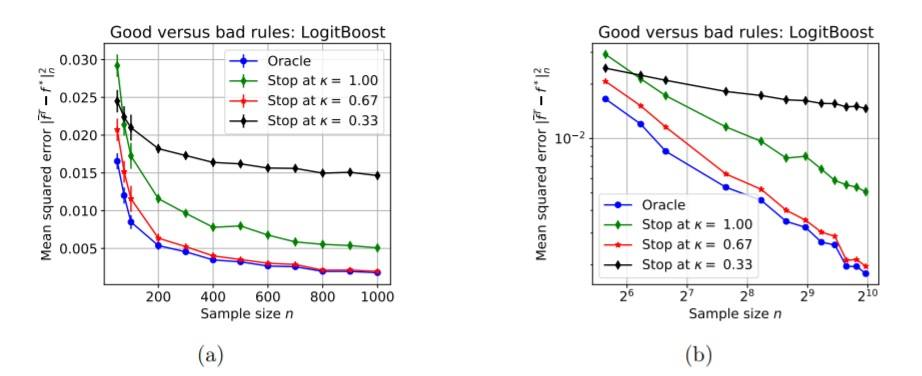
\includegraphics[width=\textwidth]{img/early_stopping_logit_plot.jpg}
  \caption{Illustration taken from \cite{wain17ada}. Mean-squared errors $||\bar{f}^T-f^*||_n^2$ for different stopping rules $T=(7n)^{\kappa}$ and the oracle gold standard (a) and in log-scale (b).}
  \label{l2boost}
\end{figure}

Indeed, the derived stopping rule using $\kappa=\frac{2}{3}$ performs best amongst the early stopping algorithms and has a performance very similar to the oracle gold standard. The slopes in the plot in log-scale confirm the different rates for the error bounds given in theorem \ref{thmbound}.

The two other stopping rules both perform worse. A stopping too early ($\kappa=\frac{1}{3}$) corresponds to underfitting, whereas stopping too late ($\kappa=1$) corresponds to overfitting.

\section{Discussion}
The results of \cite{wain17ada} also show that the derived stopping rule matches a minimax lower bound for a broad class of kernels up to constant factors and is therefore optimal. In fact, when stopping at $T=\lfloor \frac{1}{\delta_n^2 \max\{8,M\}}\rfloor$, using a stepsize of $\alpha=\frac{m}{M}$ and initialization $f^0=0$, then for any function $f^*$ with $||f^*||_{\mathcal{H}}\le 1$
\begin{equation}
\mathbb{E}||\bar{f}^T-f^*||_n^2 \asymp \inf_{\hat{f}}\sup_{||f||_{\mathcal{H}}\le 1} \mathbb{E}||\hat{f}-f^*||_n^2.
\end{equation}
Another important aspect of this paper is the role kernels play for these results.
Eigenvalue decay conditions of certain kernels can be used in order to obtain explicit bounds for the critical radius $\delta_n$, which would otherwise be hard to obtain.
Also, we used the fact that the Hilbert space $\mathcal{H}$ is an RKHS, and that we can therefore restrict our attention to the subspace $\mathcal{H}_n = \operatorname{span}(\{K(\cdot, x_i)\}_{i=1,\dots,n})$ due to the Representer theorem. This allows us to identify functions in $\mathcal{H}_n$ with vectors in $\mathbb{R}^n$, which is much more convenient to work with.

Finally, throughout these notes we assumed that the covariates $x_{i}$ are fixed.
It is also shown in \cite{wain17ada} that this condition can be relaxed.
Define the $L_{2}(\mathbb{P}_{X})$ norm as $\norm{\cdot}_{2}$ to be given by
$$
\norm{\hat{f} - f^{*}}_{2}^{2} = \mathbb{E}_{X}[(\hat{f}(X) - f^{*}(X))^{2}].
$$
The extension to the random design case work by relating the norms
$\norm{\cdot}_{n}$
and $\norm{\cdot}_{2}$.
In particular, let
$$
\bar{\mathcal{E}}(\delta) \coloneqq \{f^{*}-f \mid f\in\mathcal{H}, ||f^{*}-f||_{\mathcal{H}}\le 1, ||f^{*}-f||_2 \leq \delta\},
$$
and let
\begin{equation}
\bar{\mathcal{G}}_{n}(\bar{\mathcal{E}}(\delta)) \coloneqq
\mathbb{E}_{X_{1:n}, w_{1:n}}\Big[\sup_{h\in\bar{\mathcal{E}}(\delta)}\frac{1}{n}\sum_{i=1}^nw_ih(x_i)\Big],
\end{equation}
where now the expectation is taken also with respect to the covariates.
Let $\bar{\delta}_{n}$ be the identically defined critical radius with respect to
$\bar{\mathcal{G}}_{n}(\bar{\mathcal{E}}(\delta))$.
Then, the difference between the norms
$\norm{\cdot}_{n}$
and $\norm{\cdot}_{2}$ is bounded by a factor proportional to $\bar{\delta}_{n}$
and also $\delta_{n} \leq \bar{\delta}_{n}$. Combining these two facts, we get that
under the same stopping rule $T$, $\norm{\bar{f}^{T} - f^{T}}_{2}^{2} \leq c \bar{\delta}_{n}$
for some constant $c$.


%!TEX root = optimization1718.tex

\chapter{Robustness}
\emph{Speakers: Amartya Sanyal, Mario Lezcano Casado and David Martínez Rubio }\\

% Change of notation with respect to the paper to maintain the symbols we have been using in the reading group:
%   Paper                          Us
% --------------------------------------------------------------------------------
%   R(\theta)                      r(\theta)         - True risk
%     -                            R(\theta)         - Empirical risk
%   R(\theta, \mathcal{P}_n)     R(\theta, \rho)   - robust risk
%
%


\section{Introduction}
The generalization problem we have mostly been focusing on. Let $\mathcal{X}$ be a sample space $P$ an unknown distribution on $\mathcal{X}$ from which we can sample and $\Theta$ a parameter space. Given a loss function $\ell : \Theta \times \mathcal{X} \rightarrow \mathcal{R}$, we want to minimize over $\Theta$ the risk
\[
    r(\theta) := \mathbb{E}_{X\sim P} [\ell(\theta, X)]\\
\]

for solving this task, we take samples $x_1, \dots, x_n$ i.i.d. from $P$ and then one usually compute the empirical risk
\[
    R(\theta) := \frac{1}{n} \sum_{i=1}^n \ell(\theta, x_i)
\]
and minimize it over $\Theta$. In the literature we can find in different bounds contexts bounds of the following form, with high probability:
\[
    r(\theta) \leq \frac{1}{n} \sum_{i=0}^n \ell(\theta, x_i) + C_1 \sqrt{\frac{\Var(\ell(\theta, X))}{n}} + \frac{C_2}{n} \text{ for all } \theta \in \Theta
\]
where $C_1$ and $C_2$ depend on the parameters of the problem and the desired confidence guarantee. These bounds justify empirical risk minimization (ERM), i.e. minimizing $R(\theta)$. ERM is the most natural way to tackle our problem, we take an unbiased estimator of the value we want to minimize and minimize that one instead. However, while choosing $\theta$ we do not make any attempt to control the variance of our losses and thus the quantity we really want to bound could be big. 

It seems natural to ask if we can get trade-offs between bias and variance in the generalization error, or more concretely if minimizing the weighted sum
\begin{equation}\label{empirical_biased_estimator}
R(\theta) + C\sqrt{\frac{\Var_{\hat{P}_n}(\ell(\theta, X))}{n}}
\end{equation}
we can get a lower generalization error. This idea was considered previously, but unfortunately the previous expression is not necessarily convex when $\ell$ is convex.  The paper we present, \textit{Variance-based regularization with convex objectives} \cite{duchi17roubust} proposes a different estimator, convex on $\theta$, that under some assumptions it is close to \eqref{empirical_biased_estimator}. They call their estimator the \textit{robustly regularized risk} and prove some generalization guarantees depending on the Rademacher complexities, covering numbers or localized Rademacher complexities.

\section{Robustly Regularized Risk}

Before defining the robustly regularized risk, we need to define first some concepts.

Let $\phi : \mathbb{R}_+ \rightarrow \mathbb{R}$ be a convex function with $\phi(1) = 0$. Then the $\phi$-\textit{divergence} between distributions $P$ and $Q$ defined on a space $\mathcal{X}$ is 
\[
    D_{\phi}(P\|Q) = \int \phi\left(\frac{dP}{dQ} dQ\right) = \int_{\mathcal{X}} \phi\left(\frac{p(X)}{q(X)}\right) q(X) d\mu(X),
\]
where $\mu$ is any measure for which $P,Q  \ll \mu$, and $p= \frac{dP}{d\mu}$, $q = \frac{dQ}{d\mu}$. The paper makes use of the $\chi^2$-divergence, which corresponds with $\phi(t)=(t-1)^2$. Given $\phi$ and a sample $X_1, \dots, X_n$, we define the \textit{local neighborhood of the empirical distribution with radius} $\rho$ by 
\[
    \mathcal{P}_n := \left\{ \text{distributions } P \text{ such that } D_\phi\left(P \| \hat{P}_n\right)\leq \frac{\rho}{n } \right\}
\]
where $\hat{P}_n$ denotes the empirical distribution of the sample. Then, the robustly regularized risk is defined as
\[
    R_n(\theta, \rho) := \sup_{P\in\mathcal{P}_n} \mathbb{E}_P [\ell(\theta, X)] = \sup_{P}\left\{\mathbb{E}_P[\ell(\theta, X)]: D_{\phi}(P\|\hat{P}_n) \leq \frac{\rho}{n}\right\}.
\]
It is convex on $\theta$ because it is defined as the supremum of convex functions. The proposed estimation is to choose a parameter $\hat{\theta}^\rob$ that minimizes $R_n(\theta, \rho)$. The authors prove that this estimator is close to \eqref{empirical_biased_estimator}, in particular it is $O(1/n)$ lower than  \eqref{empirical_biased_estimator} uniformly in $\theta$ and if the variance of $\ell(\theta, X)$ is big enough we will see that with high probability the two estimators are the same.

\section{Variance expansion}
We want to see that the risk $R_n(\theta, \rho)$ is a good approximation to the empirical risk plus a variance term. In order to understand this kind of variance expansion it is useful to study first the following problem
\begin{align}\label{variance_expansion}
	\begin{aligned}
         &\text{maximize}_{p} \sum_{i=1}^n p_i z_i \\
         &\text{subject to } p \in \mathcal{P}_n = \left\{p\in \mathbb{R}_+^n : \frac{1}{2} \|np-\textbf{1}\|_2^2 \leq \rho, \langle \textbf{1}, p \rangle = 1\right\},
	\end{aligned}
\end{align}
where $z \in \mathbb{R}^n$ is a vector. Let $s_n^2 := \frac{1}{n} \|z\|_2^2 - (\bar{z})^2 $ be the empirical variance of the vector $z$, where $\bar{z} = \frac{1}{n} \langle \textbf{1}, z\rangle$ is the mean value of $z$. Then by introducing the variable $u=p-\frac{1}{n} \textbf{1}$, the objective in problem \eqref{variance_expansion} satisfies $\langle p, z \rangle = \bar{z} + \langle u, z \rangle = \bar{z} + \langle u, z-\bar{z} \rangle$ because $\langle u, \textbf{1}=0\rangle$. Thus problem \eqref{variance_expansion} is equivalent to solving
\[
    \text{maximize}_{u\in \mathbb{R}^n}  \bar{z} + \langle  u, z-\bar{z}\rangle \text{  subject to } \|u\|_2^2 \leq \frac{2\rho}{n^2}, \langle \textbf{1}, u\rangle = 0, u \geq -\frac{1}{n}.
\]
If there is $u \propto z-\bar{z}$ that satisfies the constraints, the maximum is attained at such vector. This would be 
\[
    u_i = \frac{\sqrt{2\rho}(z_i -\bar{z})}{n\|z-\bar{z}\|_2} = \frac{\sqrt{2\rho} (z_i -\bar{z})}{n\sqrt{ns^2_n}}.
\]
It is possible to satisfy the constraint $u_i \geq -1/n$  if and only if 
\[
    \min_{i\in [n]} \frac{\sqrt{2\rho}(z_i - \bar{z})}{\sqrt{ns_n^2}} \geq -1.
\]
Thus if variance is large enough and thus the previous inequality holds for the vector $z$ we have 
\[
    \sup_{p\in\mathcal{P}_n} \langle p, z\rangle = \bar{z} + \sqrt{\frac{2\rho s_n^2}{n}}.
\]
This will correspond to an equality between $R_n(\theta, \rho)$ and \eqref{variance_expansion} when the variance is large enough.

%!TEX root = optimization1718.tex

\chapter{Neural Networks}

\emph{Speaker:} Thomas Orton, Guillermo Valle P'{e}rez\\


\section{Introduction}

\ 

Neural networks emperically show good generalization when trained on real life data; however, we have been unable to theoretically explain why this is the case. In particular, traditional techniques which try to give generalization bounds based on the number of parameters of a neural network significantly overestimate the number of training samples required for the network to generalize. This paper does two things to help make progress in this area: 

\begin{enumerate}

\item Introduce a new conceptial "compression" framework for getting generalization bounds (section 2).

\item Give new generalization bounds for neural networks based on metrics of networks which are found to be emperically favourable when trained on real life data (section 3). 

\end{enumerate}


\section{Compression and Generalization}

\subsection{Setting and notation}

We consider a multiclass classification setting, where labels come from $\{1,...,k\}$ and for a sample $x$ we map $x \rightarrow f(x) \in \mathbb{R}^{k}$, where the classification loss is defined as

$$\mathbb{P}_{(x,y)\sim \mathcal{D}} \left[f(x)[y] <  \max_{i\neq y} f(x)[i]\right]$$

If  $\gamma>0$ is some desired margin, then the expected margin loss is

$$
L_{\gamma}(f) = \mathbb{P}_{(x,y)\sim \mathcal{D}} \left[f(x)[y] \leq \gamma + \max_{i\neq y} f(x)[i]\right]
$$

We let $\hat{L}_{\gamma}$ denote the emperical margin loss, and $L_{\gamma}$ the true margin loss. The generalization error is the difference between the two. 

\ 

\subsection{Compressibility}

The high level idea of this section is the following: Suppose we have a classifier $f$ from a complicated hypothesis class which has very low emperical loss on $m$ samples. We can try to approximate $f$ by compressing it to a function $g$, where $g$ belongs to a family of functions with fewer than $m$ effective parameters. This allows us to get generalization bounds on $g$. The following definitions make this idea formal:

\

\begin{definition}[($\gamma$,$S$)-compressible using helper string $s$] Suppose $G_{\mathcal{A},s} =\{g_{A,s}|A\in \mathcal{A}\}$ is a class of classifiers indexed by trainable parameters $A$ and fixed strings $s$.  A classifier $f$ is  ($\gamma,S$)-compressible with respect to $G_{\mathcal{A},s}$ using helper string $s$ if there exists $A\in \mathcal{A}$ such that for any $x\in S$, we have for all $y$
\begin{equation}
    |f(x)[y] - g_{A,s}(x)[y]| \le \gamma.
\end{equation}

\end{definition}

\


\begin{theorem}\label{thrm21} Suppose $G_{\mathcal{A},s} =\{g_{A,s}|A\in \mathcal{A}\}$ where $A$ is a set of $q$ parameters each of which can have at most $r$ discrete values and $s$ is a helper string. Let $S$ be a training set with $m$ samples. If the trained classifier $f$ is $(\gamma,S)$-compressible via $G_{\mathcal{A},s}$ with helper string $s$, then there exists $A\in\mathcal{A}$ s.t. with high probability over the training set,
\begin{equation}
    L_0(g_A) \le \hat{L}_\gamma(f)+ O\left(\sqrt{\frac{q\log r}{m}}\right).
\end{equation}

\end{theorem}

\begin{proof}

We can use the Chernoff bound to give 

\begin{equation}
Pr[L_{0}(g_{A}) - \hat{L}_{\gamma}(g_{A})\geq \tau ] \leq \exp(-2\tau^2 m)
\end{equation}

Choosing $\tau=\left(\sqrt{\frac{q\log r}{m}}\right)$, and taking a union bound over all $r^{q}$ different $A \in \mathcal{A}$, we have that with probability at least $1-\exp(-q\log r)$, for all $A \in \mathcal{A}$

\begin{equation}
L_{0}(g_{A}) \leq \hat{L}_{\gamma}(g_{A})+\left(\sqrt{\frac{q\log r}{m}}\right)
\end{equation}

Since $f$ is $(\gamma,\mathcal{S})-$compressible with respect to $g$, we can pick an $A \in \mathcal{A}$ such that for all $x \in S$, and any $y$, we have

\begin{equation}
|f(x)[y]-g_{A}(x)[y]|\leq \gamma
\end{equation}

For each training example, if $f$ has margin at least $\gamma$, then $g_{A}$ also classifies this example correctly. Thus

\begin{equation}
\hat{L}_{0}(g_{A})\leq \hat{L}_{\gamma}(f)
\end{equation}

\end{proof}

\textbf{Comment}: In the setting of Theorem 2.1, if the compression works for $1-\zeta$ fraction of the training sample, then with high probability
$$
    L_0(g_A) \le \hat{L}_\gamma(f)+ \zeta+O\left(\sqrt{\frac{q\log r}{m}}\right).
    $$




\subsection{Examples}

\subsection{Example 1: Linear classifiers with margin}

Consider a binary linear classifier $c \in \mathbb{R}^{h}$, $\|c\|=1$ with high margin. Namely $c(x):=sgn(c \cdot x)$, where $\forall x,y$ we have  $\|x\|=1$, $y \in \{-1,1\}$, and for all $(x,y)\in S$ in our training set, we have $y(c^{T}x)\geq \gamma$. We can now consider how to compress such a classifier to a simpler family of classifiers:

\iffalse

\subsubsection{First compression attempt}

\begin{algorithm}
\caption{Vector-Compress($\gamma$, $c$)}
\begin{algorithmic}
\REQUIRE vector $c$ with $\|c\| \le 1$, $\eta$.
\ENSURE vector $\hat{c}$ s.t. for any fixed vector $\|u\| \le 1$, with probability at least $1-\eta$, $|c^\top u - \hat{c}^\top u| \le \gamma$. Vector $\hat{c}$ has $O((\log h)/\eta\gamma^2)$ nonzero entries. 
\FOR{$i = 1$ to $h$}
\STATE Let $z_i = 1$ with probability $p_i = \frac{2c_i^2}{\eta\gamma^2}$ (and $0$ otherwise)
\STATE Let $\hat{c}_i = z_i c_i/p_i$.
\ENDFOR
\STATE Return $\hat{c}$
\end{algorithmic}
\label{alg:vec-compress}
\end{algorithm}


(Lemma 4): Vector-Compress($\gamma$, $c$) returns a vector $\hat{c}$ such that for any fixed $u$ (independent of choice of $\hat{c}$), with probability at least $1-\eta$, $|\hat{c}^\top u - c^\top u| \le \gamma$. The vector $\hat{c}$ has at most $O((\log h)/\eta\gamma^2)$ non-zero entries with high probability.


\begin{proof}

$\forall i \in [h]$ we have $E[\hat{c}_i]=E[x_{i}c_{i}/p_i]= c_i$ and 

$$[Var[\hat{c}]]_{i,j}=E[\hat{c}_{i}\hat{c}_{j}]-E[\hat{c}_{i}]E[\hat{c}_{j}]$$

$=0$ for $i \not =j$. For $i=j$, this equals $\frac{c_i^2}{p_i^2}\times p_i -c_i^2=p_i(1-p_i) \frac{c_i^2}{p_i^2} \le \frac{2c_i^2}{p_i} \le \eta\gamma^2$

\

For any fixed vector $u$ with $\|u\|\leq1$, we have $E[\hat{c}^\top u] = c^\top u$ and $Var[\hat{c}^\top u] =u^{\top} Var[\hat{c}]u \leq \sum_{i=1}^h u_i^2 \eta\gamma^2 \leq \eta\gamma^2$. Applying Chebyshev's inequality gives $Pr[|\hat{c}^\top u - c^\top u| \ge \gamma] \le \frac{\eta\gamma^2}{\gamma^2}=\eta$.

\ 

Moreover, the expected number of non-zero entries in $\hat{c}$ is $\sum_{i=1}^h p_i=\frac{2}{\eta \gamma^2}\sum_{i=1}^h  c_i^2 \leq \frac{2}{\eta \gamma^2}$. Let $X$ be the number of non-zero entries. Then Chernoff bound gives us that

$$P\left[X>(1+O(\log(h)))\frac{2}{\eta \gamma^2}\right]\leq \left(\frac{e}{1+O(\log(h))}\right)^{\frac{2}{\eta \gamma^2}O(\log(h))}$$

Which is small since $\eta,\gamma\leq 1$. Thus we know with high probability the number of non-zero entries is at most $O((\log h)/\eta\gamma^2)$. 
\end{proof}

\ 

Next we handle the discretization:

\

Lemma: Let $\tilde{c} = \mbox{Vector-Compress}(\gamma/2, c)$. For each coordinate $i$, let $\hat{c}_i = 0$ if $|\tilde{c}_i| \ge 2\eta\gamma\sqrt{h}$, otherwise let $\hat{c}_i$ be the rounding of $\tilde{c}_i$ to the nearest multiple of $\gamma/2\sqrt{h}$. For any fixed $u$  with probability at least $1-\eta$, $|\hat{c}^\top u - c^\top u| \le \gamma$.


\begin{proof}
Let $c'$ be a truncated version of $c$: $c'_i = c_i$ if $|c_i| \ge \gamma/4\sqrt{h}$, and $c'_i = 0$ otherwise. Then $\|c'-c\| \le \sqrt{h\frac{ \gamma^2}{8h}}=\gamma/4$. By Algorithm~\ref{alg:vec-compress}, we observe that $\tilde{c} = \mbox{Vector-Compress}(\gamma/2, c')$ ($|\tilde{c}_i| \ge 2\eta\gamma\sqrt{h}$ if and only if $|c_i| \le \gamma/4\sqrt{h}$). Finally, by the rounding we know $\|\hat{c}-\tilde{c}\|\le \gamma/4$. Combining these three terms, we know with probability at least $1-\eta$,
\begin{align*}
|\hat{c}^\top u - c^\top u| &\le  |\hat{c}^\top u - \tilde{c}^\top u|+|\tilde{c}^\top u - (c')^\top u|+|(c')^\top u - c^\top u| \\
& \le \gamma/4+\gamma/2+\gamma/4 = \gamma.
\end{align*}
\end{proof}

\ 

Combining the above two lemmas, we know there is a compression algorithm with $O((\log h)/\eta\gamma^2)$ discrete parameters that works with probability at least $1-\eta$. 

\ 

Lemma: For any number of sample $m$, there is an efficient algorithm to generate a compressed vector $\hat{c}$, such that 
$$
L(\hat{c}) \le \tilde{O}((1/\gamma^2 m)^{1/3})
$$


\begin{proof}
We will choose $\eta = (1/\gamma^2 m)^{1/3}$. By the previous two lemmas, we know there is a compression algorithm that works with probability $1-\eta$, and has at most $\tilde{O}((\log h)/\eta\gamma^2)$ parameters. By Corollary~\ref{cor:compression}, we know
$$
L(\hat{c}) \le \tilde{O}(\eta + \sqrt{q/m}) = \tilde{O}\left(\eta + \sqrt{\frac{1}{\eta\gamma^2m}}\right) = \tilde{O}((1/\gamma^2 m)^{1/3} + \sqrt{1/\eta\gamma^2m}) = \tilde{O}((1/\gamma^2 m)^{1/3}).
$$
\end{proof}


Note that the rate we have here is not optimal as it depends on $m^{1/3}$ instead of $\sqrt{m}$. This is mostly due to cannot give a high probability bound (indeed if we consider all the basis vectors as the test vectors $u$, Vector-Compress is always going to fail on some of them). 

\fi

\begin{algorithm}
\caption{Vector-Project($\gamma$, $c$)}
\begin{algorithmic}
\REQUIRE vector $c$ with $\|c\| \le 1$, $\eta$.
\ENSURE vector $\hat{c}$ s.t. for any fixed vector $\|u\| \le 1$, with probability at least $1-\eta$, $|c^\top u - \hat{c}^\top u| \le \gamma$. 
\STATE Let $k = 16\log(1/\eta)/\gamma^2$
\STATE Sample $k$ random Gaussian vectors $v_1,...,v_k\sim N(0,I)$.
\STATE Compute $z_i = \langle v_i,c\rangle$
\STATE (Optional): Round $z_i$ to the closes multiple of $\gamma/2\sqrt{hk}$.
\STATE Return $\hat{c} = \frac{1}{k}\sum_{i=1}^k z_i v_i$
\end{algorithmic}
\label{alg:vec-proj}
\end{algorithm}

\ 

\begin{lemma} For any fixed vector $u$, Algorithm $\mbox{Vector-Project}(c, \gamma)$ produces a vector $\hat{c}$ such that with probability at least $1-\eta$, we have $|\hat{c}^\top u - c^\top u| \le \gamma$.

\end{lemma}

\ 

\begin{proof}
This is in fact a well-known corollary of Johnson-Lindenstrauss Lemma. Observe that 

\begin{equation}
\hat{c}^\top u = \frac{1}{k} \sum_{i=1}^k \langle v_i,c\rangle\langle v_i,u\rangle
\end{equation}


The expectation $E[\langle v_i,c\rangle \langle v_i,u\rangle] = E[c^\top v_iv_i^\top u] = c^\top E[v_iv_i^\top] u = c^\top u$. Also

\begin{align*}
Var[\frac{1}{k} \sum_{i=1}^k \langle v_i,c\rangle\langle v_i,u\rangle]&=\frac{1}{k} Var[\langle w,c\rangle\langle w,u\rangle]\\
&\leq \frac{1}{k}E\left [ ((c^{T} w)(u^{T} w))^{2}\right]\\
=&\frac{1}{k}E\left[\sum_{i,j,k,l} c_{i} c_{j} u_{k} u_{l} w_{i} w_{j}w_{k}w_{l}\right]\\
&\leq \frac{1}{k}\left[E\left[\sum_{i,k} c_{i}^2 u_{k}^2 w_{i}^2 w_{k}^2\right]+2E\left[\sum_{i,k} c_{i}u_{i} c_{k}u_{k} w_{i}^2w_{k}^2\right]\right]\\
=&O\left(\frac{1}{k}\right)\left [\sum_{i,k} c_{i}^2 u_{k}^2+\sum_{i,k} c_{i}u_{i} c_{k}u_{k}\right]=O\left(\frac{1}{k}\right)
\end{align*}

Since $c,u$ have norm less than $1$, and $\sum_{i} c_iu_i \leq \|c\|\|u\|$. 

\ 

%$O(1/k)\le O(\gamma/\sqrt{\log n})$. 

Standard concerntration inequalities give that
\begin{equation}
\Pr[|\hat{c}^\top u - c^\top u| > \gamma/2] \le \exp(-\gamma^2k/16)= \exp(\log(\eta))=\eta.
\end{equation}

\ 

It remains to show that by rounding $z_i$ to the closest multiples of $\gamma/2\sqrt{hk}$, our error increases by at most $\gamma/2$. 

\

\textbf{Claim:} a matrix with $i.i.d.$ Consider the matrix $V$ with columns $v_1,...,v_k$. Then with high probability, its spectral norm is at most $2\sqrt{h}$. 

\

Notice that $\hat{c}=Vz$, where $z$ is the vector of the $z_i$'s. If the spectral norm of $V$ is at most $2\sqrt{h}$, then changing each $z_i$ coordinate-wise by at most $\gamma/4\sqrt{hk}$ can change $\hat{c}$ in $l_2$ norm by at most $\gamma/2$.

\ 


\end{proof}

\

\begin{lemma} For any number of sample $m$, there is an efficient algorithm with helper string to generate a compressed vector $\hat{c}$, such that 
\begin{equation}
L(\hat{c}) \le \tilde{O}(\sqrt{1/\gamma^2 m}).
\end{equation}

\end{lemma}

\begin{proof}
We will choose $\eta = 1/m$. By Lemma, we know there is a compression algorithm that works with probability $1-\eta$, and has at most $O((\log 1/\eta)/\gamma^2)$ parameters. By Corollary, we know
$$
L(\hat{c}) \le \tilde{O}(\eta + \sqrt{1/\gamma^2m}) \le \tilde{O}(\sqrt{1/\gamma^2 m}).
$$
\end{proof}


\subsection{Example 2: Existing generalization bounds}

\textbf{Notation:} We define the outputs of the ith layer of a neural network by $x^{i}=A^{i} \phi (x^{i-1})$, where $\phi$ is a RelU activation function. 

\

\begin{theorem} A deep net with layers $A^1, A^2, \ldots A^d$ 
and output margin $\gamma$ on a training set $S$, the generalization error can be bounded by


\begin{equation}
\tilde{O}\left(\sqrt{\frac{hd^2\max_{x\in S}\|x\| \prod_{i=1}^{d} \|A^i\|_2^2 \sum_{i=1}^d \frac{\|A^i\|_F^2}{\|A^i\|_2^2}}{\gamma^2m}}\right).
\end{equation}

\end{theorem}



Note that ($\sum_{i=1}^d \frac{\|A^i\|_F^2}{\|A^i\|_2^2}$) is  sum of stable ranks of the layers, and that ($\prod_{i=1}^{d} \|A^i\|_2^2$) is the maximum norm of the vector it can produce if the input is a unit vector. The Lipschitz constant of the full network is at most $\prod_{i=1}^d \|A^i\|_2.$ 

\ 

We prove the theorem in two steps. First, we want to compress a matrix $A$ to a low rank matrix $\hat{A}$. In particular, if $\hat{A}$ has rank $r$, it can be expressed as a product of two matrices $B_1,B_2$ of inner dimension $r$, and so $\hat{A}$ has $2hr$ parameters. We can then round the entries of $B_1,B_2$ to compress $A$ to a finite set of functions. The second step is to show that if we replace the layers $\{A^{i}\}$ by $\{\hat{A}_{i}\}$, then the output of our network doesn't change significantly. 

\

\begin{lemma} For any matrix $A\in \mathbb{R}^{m\times n}$, let $\hat{A}$ be the truncated version of $A$ where singular values that are smaller than $\delta\|A\|_2$ are removed. Then $\|\hat{A}-A\|_2\leq \delta\|A\|_2$ and $\hat{A}$ has rank at most $\|A\|_F^2/(\delta^2\|A\|_2^2)$.
\end{lemma}


\begin{proof}
Let $r$ be the rank of $\hat{A}$. By construction, the maximum singular value of $\hat{A}-A$ is at most $\delta\|A\|_2$. Since the remaining singular values are at least $\delta\|A\|_2$, we have $\|A\|_F \ge \|\hat{A}\|_F \ge \sqrt{r} \delta\|A\|_2$. These inequalities come from that fact that if $A=UDV^{T}$ is the SVD of $A$ with singular values $\{\delta_i\}$, then 

\begin{equation}
\|A\|_{F}^2 = tr[AA^{T}]=tr[UDV^{T}VD^{T}U^{T}]=tr[DD^{T}U^{T}U]=tr[DD^{T}]=\sum_{i} \delta_{i}^2
\end{equation}

i.e. the frobenius norm squared of a matrix is just the sum of the squared signular values of that matrix. 

\end{proof}

\begin{lemma} Let $f^{i}_{A}$ denote the output of the $i$th layer a $d$ layer neural network with layers $A^{1},...,A^{d}$. Let $\Delta_i= \|f^i_{A+B}(x)-f^i_{A}(x)\|_2$. Suppose for all layers $i$ we have $\|B^{i}\|\leq \frac{1}{d}\|A^{i}\|$. Then:
\begin{equation*}
\Delta_i \leq \left(1+\frac{1}{d}\right)^i \left(\prod_{j=1}^i \|A_j\|_2\right)\|x\|_2\sum_{j=1}^i \frac{\|B_j\|_2}{\|A_j\|_2}.
\end{equation*}
\end{lemma}

\begin{proof}
For the induction case:
\begin{align*}
\Delta_{i+1} &= \|\left(A^{i+1}+B^{i+1}\right)\phi_i(f^i_{A+B}(x))- A^{i+1}\phi_i(f^i_{A}(x))\|_2 \\
&= \|\left(A^{i+1}+B^{i+1}\right)\left(\phi_i(f^i_{A+B}(x))- \phi_i(f^i_{A}(x))\right)+ B^{i+1}\phi_i( f^i_{A}(x))\|_2\\ 
&\leq \left(\|A^{i+1}\|_2+\|B^{i+1}\|_2\right)\|\phi_i(f^i_{A+B}(x))- \phi_i(f^i_{A}(x))\|_2+ \|B^{i+1}\|_2\|\phi_i(f^i_{A}(x))\|_2\\ 
&\leq \left(\|A^{i+1}\|_2+\|B^{i+1}\|_2\right)\|f^i_{A+B}(x)-f^i_{A}(x)\|_2+ \|B^{i+1}\|_2\|f^i_{A}(x)\|_2\\
&=\Delta_i\left(\|A^{i+1}\|_2+\|B^{i+1}\|_2\right)+ \|B^{i+1}\|_2\|f^i_{A}(x)\|_2,
\end{align*}


And so we get

\begin{align*}
\Delta_{i+1} &\leq \Delta_i\left(1+\frac{1}{d}\right)\|A^{i+1}\|_2+ \|B^{i+1}\|_2 \|x\|_2\prod_{j=1}^i \|A^j\|_2\\
&\leq \left(1+\frac{1}{d}\right)^{i+1} \left(\prod_{j=1}^{i+1}\|A^j\|_2\right)\|x\|_2\sum_{j=1}^i \frac{\|B^j\|_2}{\|A^j\|_2}+ \frac{\|B^{i+1}\|_2}{\|A^{i+1}\|_2}\|x\|_2\prod_{j=1}^{i+1}\|A^i\|_2\\
&\leq \left(1+\frac{1}{d}\right)^{i+1} \left(\prod_{j=1}^{i+1}\|A^j\|_2\right)\|x\|_2\sum_{j=1}^{i+1} \frac{\|B^j\|_2}{\|A^j\|_2}
\end{align*}
\end{proof}


Combining these lemmas, we can prove the theorem:

\begin{proof}
For each $i$, replace $A^{i}$ by its compression $\hat{A}^{i}$ with parameter $\delta=\gamma \max_{x} (e\|x\|d\prod_{i=1}^d \|A^{i}\|_{2})^{-1}$. The network $f_{\hat{A}}$ then has error at most 

\begin{equation*}
\Delta_{d} \leq e \left(\prod_{j=1}^d \|A_j\|_2\right)\|x\|_2\sum_{j=1}^d \frac{\|\hat{A}_j-A_{j}\|_2}{\|A_j\|_2}\leq e \left(\prod_{j=1}^d \|A_j\|_2\right)\|x\|_2d\delta=\gamma.
\end{equation*}

and the total number of parameters of the network is at most 

\begin{equation*}
\sum_{i=1}^d \frac{\|A\|_F^2}{(\delta^2\|A\|_2^2)} 2h=2h \delta^{-2}\sum_{i=1}^d \frac{\|A\|_F^2}{(\delta^2\|A\|_2^2)} = 2e^{2}d^2 h\|x\|^2\prod_{i=1}^d \|A^{i}\|^{2}_{2}\sum_{i=1}^d \frac{\|A^{i}\|^{2}_{F}}{\|A^{i}\|^{2}_{2}}/\gamma^2.
\end{equation*}


\textbf{Claim:} We can round the weights in the rank $r$ representation of each $\hat{A}_{i}$ to the nearest $\|A\|_{F}/h^{2}$ while keeping the approximation error sufficiently small. Note that the precise parameters for how we discretize will ordinarily not show up in the $\tilde{O}$ term, because there is only a logarithmic dependence of the model complexity on the number of discrete values each parameter has. 


\ 

Applying our $(\gamma,S)$-compressibility theorem from the previous section, we get that our compressed net has error at most 

\begin{equation}
L_{0}(g_{A}) \leq \hat{L}_{\gamma}(f)+\tilde{O}\left(\sqrt{\frac{hd^2\max_{x\in S}\|x\| \prod_{i=1}^{d} \|A^i\|_2^2 \sum_{i=1}^d \frac{\|A^i\|_F^2}{\|A^i\|_2^2}}{\gamma^2m}}\right)
\end{equation}

Since $f$ has output margin $\gamma$, it has the same error as $g_{A}$, and hence the same generalization bound applies.

\end{proof}

\textbf{Comment:} There is a technical issue with the above proof as presented in the paper, which requires us to be careful when invoking $(\gamma,S)$-compressibility. In particular, we are supposed to only choose the set of models we compress $f$ to $\textbf{before}$ we see the training set, but the above proof chooses this set based on properties of $f$ after training. In order to deal with this, we should really choose the rank $r$ and precision of descritization we compress our matrices to in advance, and then get a generalization bound based on this choice assuming we can compress $f$ to this set of models we chose in advance. 

\section{Definition of quantities measuring noise sensitivity}

These are quantities measuring the sensitivity to noise of the neural network, and which are used in proving Theorem~\ref{fc-net-theorem}. 

    Let $S$ be the training set.
    \begin{enumerate}
        \item {\bf Layer cushion ($\mu_{i}$)}: For any layer $i$, we define the layer cushion $\mu_i$ as the largest number such that for any $x\in S$:
        $$
        \mu_{i}\|A^i\|_F\|\phi(x^{i-1})\| \leq \|A^i\phi(x^{i-1})\|
        $$
        \item {\bf Interlayer cushion ($\mu_{i,j}$)}: For any two layers $i\leq j$, we define interlayer cushion $\mu_{i,j}$ as the largest number such that for any $x\in S$:
        $$
        \mu_{i,j}\|J^{i,j}_{x^i}\|_F\|x^i\| \leq  \|J^{i,j}_{x^i}x^i\|
        $$
        Furthermore, we define minimal interlayer cushion $\icu = \min_{i\leq j\leq d} \mu_{i,j} = \min\{1/\sqrt{h^i},\min_{i< j\leq d} \mu_{i,j}\}$.
        \item {\bf Activation contraction ($c$)}: The activation contaction $c$ is defined as the smallest number such that for any layer $i$ and any $x\in S$,
        $$
        \|x^i\| \leq c \|\phi(x^i)\|
        $$
        \item {\bf Interlayer smoothness ($\rho_{\delta}$)}: Interlayer smoothness is defined the smallest number such that with probability $1-\delta$ over noise $\eta$ for any two layers $i<j$ any $x\in S$:
        $$
        \|M^{i,j}(x^{i}+\eta)-J_{x^i}^{i,j}(x^{i}+\eta)\| \leq \frac{\|\eta\|\|x^{j}\|}{\rho_{\delta}\|x^{i}\|}
        $$
    \end{enumerate}


\section{Fully connected networks}

The intuition behind this result is that if we can find a network $f_{\tilde{A}}$, which does well on the training set, and belongs to a small hypothesis class (independent of the training set), then we can bound its generalization error. The way we ensure it does well on the training set is by ensuring its outputs are not very different from $f_A$ which already does well on the training set (if $\hat{L}_{\gamma}(f_A)$ is small). The way we ensure it belongs to a small hypothesis class is by constructing $f_{\tilde{A}}$ in a way that it is parametrized by few parameters

\begin{theorem}\label{fc-net-theorem} For any fully connected network $f_A$ with $\rho_\delta \geq 3d$, any probability $0 < \delta \leq 1$ and any margin $\gamma$, Algorithm~\ref{alg:matrix-proj} generates weights $\tilde{A}$ for the network $f_{\tilde{A}}$ such that with probability $1-\delta$ over the training set and $f_{\tilde{A}}$ , the expected error $L_0(f_{\tilde{A}})$ is bounded by 
\begin{equation*}
    \hat{L}_\gamma(f_A) + \tilde{O}\left ( \sqrt{\frac{c^2 d^2 \max_{x \in S} || f_A(x) ||_2^2 \sum_{i=1}^d \frac{1}{\mu_i^2 \mu^2_{i\rightarrow}}}{\gamma^2 m}} \right)
\end{equation*}

where $\mu_i$, $\mu_{i\rightarrow}$, $c$ and $\rho_\delta$ are layer cushion, interlayer cushion, activation contraction and interlayer smoothness.

\end{theorem}

\begin{algorithm}
    \caption{Matrix-Project ($A$, $\eps$, $\eta$)}
    \begin{algorithmic}
        \REQUIRE Layer matrix $A\in \R^{h_1\times h_2}$, error parameter $\eps$, $\eta$.
        \ENSURE Returns $\hat{A}$ s.t. $\forall$ fixed vectors $u,v$, $$\Pr[|u^\top \hat{A} v - u^\top Av\| \ge \eps\|A\|_F\|u\|\|v\|] \le \eta.$$
        \STATE Sample $k = \log(1/\eta)/\eps^2$ random matrices $M_1,\dots,M_k$ with entries i.i.d. $\pm 1$ (\textquotedblleft helper string\textquotedblright)
        \FOR{$k'=1$ to $k$}
        \STATE Let $Z_{k'} = \inner{A,M_{k'}} M_{k'}$.
        \ENDFOR
        \STATE Let $\hat{A} =\frac{1}{k}\sum_{k'=1}^k Z_{k'}$
    \end{algorithmic}
    \label{alg:matrix-proj}
\end{algorithm}


To prove this, the crucial step is to show that $f_A$ can be ``compressed'' to a $f_{\tilde{A}}$ with less parameters. This means that the output of $f_{\tilde{A}}$ doesn't differ much from $f_A$ for any input in the training set $x \in S$. This will be shown in Lemma 3 (which relies on Lemma 2). This in turn means that $f_{\tilde{A}}$ can't do much worse than $f_A$ on the training set, in the sense that its margin can't be much smaller than that for $f_A$, which will allow us to say $\hat{L}_0(f_{\tilde{A}}) \leq \hat{L}_\gamma(f_{A})$, shown in Lemma 10. Finally, by using an $\epsilon$-cover of the hypothesis class of $f_{\tilde{A}}$, we can bound the difference between $\hat{L}_0(f_{\tilde{A}})$ and $L_0(f_{\tilde{A}})$ which depends on the number of parameters of $f_{\tilde{A}}$, proving Theorem 4.1.

We begin with the technical Lemma~\ref{lem:perturblayer:highprob}

\begin{lemma}\label{lem:perturblayer:highprob}
For any $0<\delta,\eps\leq 1$, et $G=\{(U^i,x^i)\}_{i=1}^m$ be a set of matrix/vector pairs of size $m$ where $U\in\R^{n\times h_1}$ and $x\in\R^{h_2}$, let $\hat{A}\in \R^{h_1\times h_2}$ be the output of Algorithm~\ref{alg:matrix-proj} with $\eta = \delta/mn$ and $\Delta = \hat{A} - A$. With probability at least $1-\delta$ we have for any $(U,x)\in G$, $\|U \Delta x\| \leq \eps\|A\|_F\|U\|_F\|x\|$.
\end{lemma}

\begin{proof}
For any fixed vectors $u,v$, we have (from definition of $\hat{A}$ by Algorithm~\ref{alg:matrix-proj})
$$
u^\top \hat{A}v = \frac{1}{k}\sum_{k'=1}^k u^\top Z_{k'} v = \frac{1}{k} \sum_{k'=1}^k \inner{A,M_{k'}}\inner{uv^\top, M_{k'}}.
$$

This is a sum of independent terms (as the $M_{k'}$ are independent). Furthermore, its expected value is 

\begin{align*}
E\left[ \frac{1}{k} \sum_{k'=1}^k \inner{A,M_{k'}}\inner{uv^\top, M_{k'}} \right] =
 \frac{1}{k} \sum_{k'=1}^k E\left[ \inner{A,M_{k'}}\inner{uv^\top, M_{k'}} \right] = \inner{A,uv^\top}
 \end{align*}
 
 where the last equality is because only the terms involving the same element of $M_{k'}$ contribute to the expectation. We can then use Hoeffding's inequality
 
 $$Pr\left[ | \frac{1}{k} \sum_{k'=1}^k \inner{A,M_{k'}}\inner{uv^\top, M_{k'}} - \inner{A,uv^\top}| \geq \eps h^2 \|A\|_F \|uv^\top\|_F \right] \leq 2 e^{-k \eps^2/2},$$
 
\textbf{This is not exactly what they got. In particular that $h^2$ which is $\max{\|M_{k'}\|_F}$. I'm going to ignore this difference in the rest of the section..} as $|\inner{A,M_{k'}}\inner{uv^\top, M_{k'}}| \leq h^2 \|A\|_F \|uv^\top\|_F $

Therefore for the choice of $k=\log(1/\eta)/\eps^2$ we know
    $$\Pr\left[|u^\top \hat{A} v - u^\top Av\| \ge \eps\|A\|_F\|u\|\|v\|
    \right] \le \eta.$$

    Now for any pair of matrix/vector $(U,x)\in G$, let $u_i$ be the $i$-th row of $U$. There are $mn$ such rows, and the inequality of interest holds with probability $\eta=\frac{\delta}{mn}$ for each. Therefore, by union bound we know with probability at least $1-\delta$ for all $u_i$ we have $|u_i^\top \Delta v\| \le \eps\|A\|_F\|u_i\|\|v\|$. Since $\|U\Delta x\|^2 = \sum_{i=1}^n (u_i^\top \Delta x)^2$ and $\|U\|_F^2 = \sum_{i=1}^n \|u_i\|^2$, we immediately get
    $\|U \Delta x\| \ge \eps\|A\|_F\|U\|_F\|x\|$.


\end{proof}

Now, we show Lemma~\ref{lem:rotate-compress}, which shows that the compressed network doesn't differ much in its outputs with $f_A$.

\begin{lemma}\label{lem:rotate-compress}
    For any fully connected network $f_A$ with $\rho_\delta\geq 3d$, any probability $0 < \delta \leq 1$ and any error $0< \eps \leq 1$, Algorithm~\ref{alg:matrix-proj} generates weights $\tilde{A}$ for a network with $\frac{72c^2d^2\log (mdh/\delta)}{\eps^2}\cdot \sum_{i=1}^d \frac{1}{\mu_i^2\mu_{i\rightarrow}^2}$ total parameters such that with probability $1-\delta/2$ over the generated weights $\tilde{A}$, for any $x\in S$:
    $$
    \|f_A(x) - f_{\tilde{A}}(x)\| \le \eps\|f_A(x)\|.
    $$
    where $\mu_i$, $\mu_{i\rightarrow}$, $c$ and $\rho_{\delta}$ are layer cushion, interlayer cushion, activation contraction and interlayer smoothness.
\end{lemma}

\begin{proof}
This is proven by induction on the layers $i$. For any layer $i\geq 0$, let $\hat{x}^j_i$ be the output at layer $j$ if the weights $A^1,\dots,A^i$ in the first $i$ layers are replaced with $\tilde{A}^1,\dots,\tilde{A}^i$. The induction hypothesis is then the following:

    Consider any layer $i\geq 0$ and any $0<\eps\leq 1$. The following is true with probability $1-\frac{i\delta}{2d}$ over $\tilde{A}^1,\dots,\tilde{A}^i$ for any $j\geq i$:
    $$
    \|\tilde{x}^j_i - x^j\|\le (i/d)\eps\|x^j\|.
    $$

    For the base case $i = 0$, since we are not perturbing the input, the inequality is trivial. Now assuming that the induction hypothesis is true for $i-1$, we consider what happens at layer $i$. Let $\tilde{A}^i$ be the result of Algorithm~\ref{alg:matrix-proj} on $A^i$ with $\eps_i=\frac{\eps\mu_i\icu}{4cd}$ and $\eta = \frac{\delta}{6d^2h^2m}$ (\textbf{not sure why this choice of $\eta$}). Now let's analyze the difference in activations between the network with the extra perturbation and the unperturbed network. For any $j \ge i$ we have, using the triangle inequality
    \begin{equation}
    \|\tilde{x}^j_i - x^j\| = \|(\tilde{x}^j_i - \tilde{x}^j_{i-1})+(\tilde{x}^j_{i-1} - x^j)\| \leq \|(\tilde{x}^j_i - \tilde{x}^j_{i-1})\| +\|\tilde{x}^j_{i-1} - x^j\|.
    \label{eq:activation-error}
    \end{equation}
    The second term can be bounded by $(i-1)\eps\|x^j\|/d$ by the induction hypothesis. Therefore, in order to prove the induction, it is enough to show that the first term is bounded by $\eps/d \|x^j\|$. 

    First, we define some notation. For any two layer $i\leq j$, denote by $M^{i,j}$ the operator for composition of these layers and $J^{i,j}_x$ be the Jacobian of this operator at input $x$ (a matrix whose $p, q$ is the partial derivative of the $p$th output coordinate with respect to the $q$'th input input). Therefore, we have $x^j = M^{i,j}(x^i)$\footnote{Remember that $x^i$ are the preactivations feeding into layer $i$}. Furthermore, since the activation functions are ReLU, we have $M^{i,j}(x^i) =J^{i,j}_{x^i} x^i$.

    We decompose the first term in Eq.~\ref{eq:activation-error} into two error terms one of which corresponds to the error propagation through the network if activation (which ReLU units are $0$) were fixed and the other one is the error caused by change in the activations:
    \begin{align*}
    \|(\tilde{x}^j_i - \tilde{x}^j_{i-1})\|
    & = \|M^{i,j}(\tilde{A}^i \phi(\tilde{x}^{i-1})) - M^{i,j}(A^i \phi(\tilde{x}^{i-1}))\|\\
    & = \|M^{i,j}(\tilde{A}^i \phi(\tilde{x}^{i-1})) - M^{i,j}(A^i \phi(\tilde{x}^{i-1})) + J^{i,j}_{x^i}(\Delta^i \phi(\tilde{x}^{i-1})) - J^{i,j}_{x^i}(\Delta^i \phi(\tilde{x}^{i-1}))\| \\
    & \leq \|J^{i,j}_{x^i}(\Delta^i \phi(\tilde{x}^{i-1}))\| + \|M^{i,j}(\tilde{A}^i \phi(\tilde{x}^{i-1})) - M^{i,j}(A^i \phi(\tilde{x}^{i-1})) - J^{i,j}_{x^i}(\Delta^i \phi(\tilde{x}^{i-1}))\| 
    \end{align*}

    where $\Delta^i = \tilde{A}^i - A^i$. To bound the first term, we can apply Lemma~\ref{lem:perturblayer:highprob} with the set $G=\{(J^{i,j}_{x^i},x^i)|x\in S,j\geq i\}$ which has size at most $dm$ (at most $d$ $J^{i,j}_{x^i}$ for each of the $m$ $x_i$). We will also need to define several quantities that measure how much error propagates through the network. The term can be bounded as follows:
    \begin{align*}
    & \|J^{i,j}_{x^i}\Delta^i \phi(\tilde{x}^{i-1})\|\\
    & \le (\eps\mu_i\icu/6cd)\|J^{i,j}_{x^i}\|_F\|A^i\|_F\|\phi(\tilde{x}^{i-1})\|&& \mbox{Lemma~\ref{lem:perturblayer:highprob}}\\
    & \le (\eps\mu_i\icu/6cd)\|J^{i,j}_{x^i}\|\|A^i\|_F\|\tilde{x}^{i-1}\|&& \mbox{Lipschitzness of the activation function}\\
    &\le (\eps\mu_i\icu/3cd)\|J^{i,j}_{x^i}\|_F\|A^i\|_F\|x^{i-1}\|&& \mbox{Induction hypothesis} \\
    &\le (\eps\mu_i\icu/3d)\|J^{i,j}_{x^i}\|_F\|A^i\|_F \|\phi(x^{i-1})\|&& \mbox{Activation Contraction} \\
    &\le (\eps\icu/3d)\|J^{i,j}_{x^i}\|_F\|A^i \phi(x^{i-1})\|&& \mbox{Layer Cushion} \\
    & = (\eps\icu/3d)\|J^{i,j}_{x^i}\|_F\|x^i\|&& x^i = A^i\phi(x^{i-1})\\
    & \le (\eps/3d) \|x^j\|&& \mbox{Interlayer Cushion} 
    \end{align*}

    \textbf{where this holds with probability $1-\frac{\delta}{6dh}$, I think.., because of the first step. However, we want it to hold with probability $1-\frac{\delta}{2d}$ for them to add up correctly?}. The second term can be bounded as:
    \begin{align*}
    & \|M^{i,j}(\tilde{A}^i \phi(\tilde{x}^{i-1})) - M^{i,j}(A^i \phi(\tilde{x}^{i-1})) - J^{i,j}_{x^i}(\Delta^i\phi( \tilde{x}^{i-1}))\| \\
    & = \|(M^{i,j}-J^{i,j}_{x^i})(\tilde{A}^i \phi(\tilde{x}^{i-1})) - (M^{i,j}-J^{i,j}_{x^i})(A^i \phi(\tilde{x}^{i-1}))\| \\
    & \leq \|(M^{i,j}-J^{i,j}_{x^i})(\tilde{A}^i \phi(\tilde{x}^{i-1}))\| + \|(M^{i,j}-J^{i,j}_{x^i})(A^i \phi(\tilde{x}^{i-1}))\|.
    \end{align*}
    Both terms can be bounded using interlayer smoothness condition of the network.
    First, notice that $A^i\phi(\tilde{x}^{i-1}) = \tilde{x}^i_{i-1}$.
    Therefore, using by induction hypothesis $\|A^i\phi(\tilde{x}^{i-1}) - x^i\| = \|\tilde{x}^i_{i-1} - x^i\| \le (i-1)\eps\|x^i\|/d \le \eps\|x^i\|$ (as $i-1 < d$).
    
    Now by interlayer smoothness property, $\|(M^{i,j}-J^{i,j}_{x^i})(A^i \phi(\tilde{x}^{i-1}))\| \le \frac{\| \tilde{x}^i_{i-1} - x^i\| \| x^j\|}{\|x^i\| \rho_{\delta}} \le \frac{\eps \|x^i\| \| x^j\|}{\|x^i\| \rho_{\delta}} \le (\eps/3d)\|x^j\|$. (as $\rho_{\delta} \geq 3d$, by assumption)
    On the other hand, we also know $\tilde{A}^i\phi(\tilde{x}^{i-1}) = A^i\phi(\tilde{x}^{i-1}) + \Delta^i\phi(\tilde{x}^{i-1})$, therefore $\|\tilde{A}^i\phi(\tilde{x}^{i-1}) - x^i\| \le \|A^i\phi(\tilde{x}^{i-1}) - x^i\| + \|\Delta^i\phi(\tilde{x}^{i-1})\| \le ((i-1)\eps/d+\eps/3d)\|x^i\| \le \eps \|x^i\|$, so again we have $\|(M^{i,j}-J^{i,j}_{x^i})(\tilde{A}^i \phi(\tilde{x}^{i-1}))\| \le (\eps/3d)\|x^j\|$.
    
    Putting everything together completes the induction, which for the last layer gives us the desired result $\|f_A(x) - f_{\tilde{A}}(x)\| \le \eps\|f_A(x)\|$, with probability at least $1-\delta/2$.

\end{proof}

We will now demonstrate that because of the perturbed network producing similar outputs to the original network, its margin of error can't be much smaller. That means that if the original had a certain error with margin $\gamma$, the perturbed one has at most that same error, albeit with a smaller margin (but how much smaller it has to be is bounded). In particular, we focus on the zero margin loss for the perturbed network in Lemma~\ref{lem:bounding_loss}.

\begin{lemma}\label{lem:bounding_loss}
    For any fully connected network $f_A$ with $\rho_\delta\geq 3d$, any probability $0<\delta\leq 1$ and any margin $\gamma>0$, $f_A$ can be compressed (with respect to a random string) to another fully connected network $f_{\tilde{A}}$ such that for any $x\in S$, $\hat{L}_0(f_{\hat{A}}) \leq \hat{L}_{\gamma}(f_A)$ and the number of parameters in $f_{\tilde{A}}$ is at most:
    \begin{equation*}
    \tilde{O}\left(\frac{c^2d^2\max_{x\in S}\|f_A(x)\|_2^2}{\gamma^2}\sum_{i=1}^d \frac{1}{\mu_i^2\icu^2}\right)
    \end{equation*}
    where $\mu_i$, $\icu$, $c$ and $\rho_{\delta}$ are layer cushion, interlayer cushion, activation contraction and interlayer smoothness. 
% defined in Definitions~\ref{def:layercushion},\ref{def:interlayercushion},\ref{def:activationcontraction} and \ref{def:interlayersmoothness} respectively.
\end{lemma}
\begin{proof}(of Lemma~\ref{lem:bounding_loss})
    If $\gamma^2 > 2\max_{x\in S}\|f_A(x)\|_2^2$, for any pair $(x,y)$ in the training set we have $|f_A(x)[y]  - \max_{i\neq y} f_A(x)[j]|^2 \leq 2\max_{x\in S}\|f_A(x)\|_2^2 \leq \gamma^2$ which means the output margin cannot be greater than $\gamma$ and therefore $\hat{L}_{\gamma}(f_A)=1$ which proves the statement.
    
If $\gamma^2\leq 2\max_{x\in S}\|f_A(x)\|_2^2$, by setting $\eps^2 = \gamma^2/2\max_{x\in S}\|f_A(x)\|_2^2$ in Lemma~\ref{lem:rotate-compress}, we know that for any $x\in S$, $\|f_A(x) - f_{\tilde{A}}(x)\|_{2}\le \gamma/\sqrt{2}$.

For any $(x,y)$, the margin of the original network $|f_A(x)[y]  - \max_{i\neq y} f_A(x)[j]|$ can be reduced by at most $|f_A - f_{\tilde{A}}| \leq \gamma$. Therefore, if for any $(x,y)$, the margin loss on the right hand side is zero $|f_A(x)[y]  - \max_{i\neq y} f_A(x)[j]| > \gamma $, and $|f_{\tilde{A}}(x)[y]  - \max_{i\neq y} f_{\tilde{A}}(x)[j]| > 0$, and so the classification loss on the left hand size is zero. Therefore whenever $f_A$ classifies well with margin $\gamma$, $f_{\tilde{A}}$ classifies well with margin $0$, which implies the inequality.

% For any $(x,y)$, if the margin loss on the right hand side is one then the inequality holds. Otherwise, the output margin in $f_{\tilde{A}}$ is greater than $\gamma$ which means in order for classification loss of $f_{A}$ to be one, we neet to have $\|f_A(x) - f_{\tilde{A}}(x)\|_{2}> \gamma/\sqrt{2}$ which is not possible and that completes the proof.
\end{proof}

% In the worst case, where all the difference between f_A and f_tilde{A} goes to the argmax_{i\neq y}, the margin is reduced by ||f_A - f_tilde{A}||_1 \leq \gamma (see relation between 1-norm and 2-norm).
% Then, wheneber f_A gets an (x,y) right,  f_tilde{A} gets it right. also., implying the inequality in the losses (which are just probabilities of getting it wrong)

Finally, we prove Theorem~\ref{fc-net-theorem}, by bounding the difference between $\hat{L}_0(f_{\tilde{A}})$ and $L_0(f_{\tilde{A}})$ (generalization gap)

\begin{proof}(of Theorem~\ref{fc-net-theorem})
    We show the generalization by bounding the covering number of the network with weights $\tilde{A}$.
%     We already demonstrated that the original network with weights $A$ can be approximated with another network with weights $\tilde{A}$ and less number of parameters.
In order to get a covering number, we need to find out the required accuracy for each parameter in the second network to cover the original network. We start by bounding the norm of the weights $\tilde{A}^i$.

    Because of positive homogeneity of ReLU activations, we can assume without loss of generality that the network is balanced, i.e for any $i\neq j$, $\|A^i\|_F = \|A^j\|_F=\beta$ (otherwise, one could rebalance the network before approximation and cushion is invariant to this rebalancing). Therefore, for any $x\in S$ we have:
    
    $$\|A^i\| \leq \frac{\|A^i\phi(x^{i-1})\|}{\mu_i\|\phi(x^{i-1})\|} = \frac{\|x^i\|}{\mu_i\|\phi(x^{i-1})\|} \leq \frac{\|x^i\|c}{\mu_i\|x^{i-1}\|}$$
    
    which we can apply layer-wise to get:
    
    \begin{align*}
    \beta^d = \prod_{i=1}^d\|A^i\| \leq \frac{c\|x^1\|}{\|x\| \mu_1}\prod_{i=2}^d\|A^i\|\leq \frac{c^2\|x^2\|}{\|x\| \mu_1\mu_2}\prod_{i=2}^d\|A^i\|\leq \frac{c^{d} \|f_A(x)\|}{\|x\|\prod_{i=1}^d \mu_i}
    \end{align*}
    By Lemma~\ref{lem:rotate-compress}, $\|\tilde{A^i}\|_F \leq \beta(1+1/d)$ (\textbf{I can't see why this is. can show using definition with sum that $\tilde{A^i} \leq \beta h^2$..}). We know that $\tilde{A}^i = \frac{1}{k}\sum_{k'=1}^k \langle A^i, M_{k'}\rangle M_{k'}$ where $\langle A^i, M_{k'}\rangle$ are the parameters. Therefore, if $\hat{A}^i$ correspond to the weights after approximating each parameter in $\tilde{A}^i$ with accuracy $\nu$, we have:
    $\|\hat{A}^i-\tilde{A}^i\|_F \leq \sqrt{k}h\nu \leq \sqrt{q}h\nu$ where $q$ is the total number of parameters. Now by Lemma~\ref{lem:lipschitz}, we get:

    \begin{align*}
    |\ell_\gamma(f_{\tilde{A}}(x),y) -\ell_\gamma(f_{\hat{A}}(x),y)| &\leq
    \frac{2e}{\gamma}\|x\|\left(\prod_{i=1}^{d} \|\tilde{A}^i\| \right) \sum_{i=1}^d \frac{\|\tilde{A}^i-\hat{A}^i\|}{\|\tilde{A}^i\|} < \frac{e^2}{\gamma}\|x\| \beta^{d-1}\sum_{i=1}^d \|\tilde{A}^i-\hat{A}^i\|_F\\
    &\leq \frac{e^2c^d \|f_A(x)\| \sum_{i=1}^d \|\tilde{A}^i-\hat{A}^i\|_F}{\gamma\beta\prod_{i=1}^d \mu_i} \leq \frac{qh\nu}{\beta}\\
    \end{align*}
    where the last inequality is because by Lemma~\ref{lem:bounding_loss}, $\frac{e^2d \|f_A(x)\|}{\gamma\prod_{i=1}^d \mu_i } < \sqrt{q}$ (because $\|f_A(x)\| \leq \max_{x\in S} \|f_A(x)\|$), and $c^d$ was ignored because c=1 for ReLU, I think see Lipsicthzness assumption above (\textbf{I think})
    Since the absolute value of each parameter in layer $i$ is at most $\beta h$, the logarithm of number of choices for each parameter in order to get $\eps$-cover is $\log(qh^2/\eps) \leq 2\log(qh/\eps)$ which results in the covering number $2q\log(kh/\eps)$. Bounding the Rademacher complexity by Dudley entropy integral (See \href{https://cstheory.stackexchange.com/questions/40472/pac-learning-bound-with-epsilon-cover-of-hypothesis-class}{here} and \href{http://www.cs.berkeley.edu/~bartlett/courses/281b-sp06/lecture24.ps}{here}) completes the proof.
\end{proof}

% \cite{pac-based}
\begin{lemma}[\cite{neyshabur2017pac}]\label{lem:lipschitz}
    Let $f_A$ be a $d$-layer network with weights $A=\{A^1,\dots, A^d\}$. Then for any input $x$, weights $A$ and $\hat{A}$, if for any layer $i$, $\|A^i-\hat{A}^i\| \leq \frac{1}{d}\|A^i\|$, then we have:
    \begin{equation*}
    \|f_A(x)-f_{\hat{A}}(x)\|_2 \leq e\|x\|\left(\prod_{i=1}^{d} \|A^i\| \right) \sum_{i=1}^d \frac{\|A^i-\hat{A}^i\|}{\|A^i\|}
    \end{equation*}
\end{lemma}



%next line adds the Bibliography to the contents page
\addcontentsline{toc}{section}{Bibliography}

\nocite{*}
\bibliography{refs}        %use a bibtex bibliography file refs.bib
\bibliographystyle{plain}  %use the plain bibliography style

\end{document}
